



Communication is a mathematical problem. Somebody wants to say something to somebody else; between them lies a channel that is expensive, or unreliable, or overheard, or all three at once. Coding theory is the study of how to package a message so that it survives the journey, and cryptography is the study of how to package it so that only the intended recipient can read it. Both subjects turn out to be, at bottom, about the same thing: the arithmetic of finite sets, and the surprising leverage that a little algebra and a little probability give us over them.

The most striking result in the course is due to Shannon, and it says something that ought to be false. If a channel corrupts one bit in ten, entirely at random, one might reasonably guess that transmitting a long message without error requires sending it over and over again, so that the rate at which information gets through must fall to zero. It does not. There is a positive number -- the \emph{capacity} of the channel -- below which arbitrarily reliable communication is possible, and Shannon's theorem tells us exactly what that number is. What makes the proof so memorable is that it establishes the existence of extremely good codes by choosing one at random, without ever exhibiting a single one.

This article constitutes my notes for the `Coding and Cryptography' course, held in Lent 2021 at Cambridge. These notes are \emph{not a transcription of the lectures}, and differ significantly in quite a few areas. Still, all lectured material should be covered.



\section{Modelling Communication}

Before we can prove anything we need a model, and the one we shall use is the one Shannon drew in 1948. There is a \vocab{source} which produces a message; an \vocab{encoder} which turns that message into something suitable for transmission; a \vocab{channel} down which the transmission travels and in which things go wrong; a \vocab{decoder} which tries to undo the damage; and finally a \vocab{receiver}, for whom the whole business was arranged.

\begin{center}
\begin{tikzpicture}[x=1cm,y=1cm]
	\tikzset{blk/.style={draw, thin, minimum height=0.75cm, minimum width=1.5cm, inner sep=2pt, font=\small}}
	\node[blk] (s)  at (0,0)    {source};
	\node[blk] (e)  at (2.5,0)  {encoder};
	\node[blk] (ch) at (5.4,0)  {channel};
	\node[blk] (d)  at (8.3,0)  {decoder};
	\node[blk] (r)  at (10.8,0) {receiver};
	\draw[->,thin] (s)  -- node[above,font=\scriptsize] {$m$} (e);
	\draw[->,thin] (e)  -- node[above,font=\scriptsize] {$c$} (ch);
	\draw[->,thin] (ch) -- node[above,font=\scriptsize] {$r$} (d);
	\draw[->,thin] (d)  -- node[above,font=\scriptsize] {$\hat m$} (r);
	\node[font=\small] (n) at (5.4,1.5) {noise};
	\draw[->,thin] (n) -- (ch);
	\node[font=\small] (ev) at (5.4,-1.5) {Eve};
	\draw[->,thin,dashed] (ch) -- (ev);
\end{tikzpicture}
\end{center}

By long-standing convention the source is called Alice, the receiver is called Bob, and any third party listening in on the channel is called Eve. The two halves of the course correspond to the two things that can go wrong in the middle of that diagram. In coding theory the enemy is the noise, and we want the message to arrive \emph{economically} and \emph{reliably}. In cryptography the enemy is Eve, and we want the message to arrive \emph{privately}.

It is worth separating two quite different problems which are often confused. \vocab{Noiseless coding}, or source coding, is about compression: we want to spend as few symbols as possible on a message, and it is adapted to the \emph{source}. Morse code is the canonical example -- the letter E, the commonest letter in English, gets the single dot, and the letter Q gets four symbols. \vocab{Noisy coding}, or channel coding, is about redundancy: we want to add enough extra symbols that corruption can be spotted and undone, and it is adapted to the \emph{channel}.

\begin{example}[ISBNs]
	Every book (before 2007) carried a ten-digit International Standard Book Number $a_1 a_2 \dots a_{10}$, where $a_1, \dots, a_9 \in \{0, 1, \dots, 9\}$ and $a_{10} \in \{0, 1, \dots, 9, X\}$, subject to the single condition
	$$\sum_{j=1}^{10} j a_j \equiv 0 \pmod{11}.$$
	Here $X$ stands for $10$, and the modulus $11$ is prime, which is what makes everything work. Suppose one digit is mistyped, say $a_k$ becomes $a_k'$. Then the check sum changes by $k(a_k - a_k')$, and since $1 \le k \le 10$ and $\abs{a_k - a_k'} \le 10$, neither factor is divisible by $11$, so the sum is no longer $0$ modulo $11$ and the error is detected. Similarly, if two adjacent digits are transposed, say $a_k$ and $a_{k+1}$ swap, the sum changes by $a_{k+1} - a_k$, again nonzero modulo $11$ unless the digits were equal in the first place.

	The channel here is a human being reading a number off a page and typing it into a computer, and the code is beautifully adapted to the errors that channel makes.
\end{example}

We now make the notion of a channel precise.

\begin{definition}[Communication Channel]
	A \vocab{communication channel} accepts strings of symbols from a finite \vocab{input alphabet} $\Ac = \{a_1, \dots, a_r\}$ and outputs strings of symbols from a finite \vocab{output alphabet} $\Bc = \{b_1, \dots, b_s\}$. It is specified by the probabilities
	$$\PP(y_1 \dots y_n \text{ received} \mid x_1 \dots x_n \text{ sent}).$$
\end{definition}

In this generality nothing can be said, because the channel is allowed to remember everything it has ever done. Almost always we assume much more.

\begin{definition}[Discrete Memoryless Channel]
	A \vocab{discrete memoryless channel} (DMC) is a channel for which the probabilities
	$$p_{ij} = \PP(b_j \text{ received} \mid a_i \text{ sent})$$
	are the same on every use of the channel, and are independent of all past and future uses. The $r \times s$ matrix $P = (p_{ij})$ is the \vocab{channel matrix}; each of its rows sums to $1$.
\end{definition}

Two examples will accompany us for the rest of the course.

\begin{example}[Binary Symmetric Channel]
	The \vocab{binary symmetric channel} (BSC) with error probability $p \in [0,1]$ has $\Ac = \Bc = \{0,1\}$ and channel matrix
	$$P = \begin{pmatrix} 1-p & p \\ p & 1-p\end{pmatrix}.$$
	Each bit is flipped independently with probability $p$, and transmitted faithfully with probability $1-p$.

	\begin{center}
	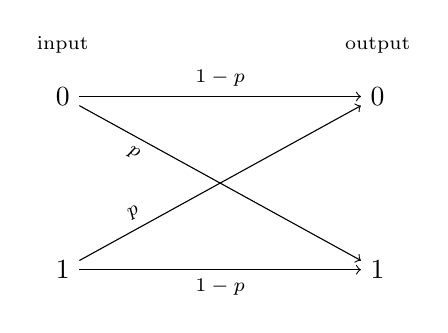
\begin{tikzpicture}[x=1cm,y=1cm]
		\node (i0) at (0,1.1)  {$0$};
		\node (i1) at (0,-1.1) {$1$};
		\node (o0) at (4,1.1)  {$0$};
		\node (o1) at (4,-1.1) {$1$};
		\draw[->,thin] (i0) -- node[above,font=\scriptsize] {$1-p$} (o0);
		\draw[->,thin] (i1) -- node[below,font=\scriptsize] {$1-p$} (o1);
		\draw[->,thin] (i0) -- node[pos=0.22,below,font=\scriptsize,sloped] {$p$} (o1);
		\draw[->,thin] (i1) -- node[pos=0.22,above,font=\scriptsize,sloped] {$p$} (o0);
		\node[font=\scriptsize] at (0,1.75) {input};
		\node[font=\scriptsize] at (4,1.75) {output};
	\end{tikzpicture}
	\end{center}

	We shall almost always assume $p < \tfrac12$. This costs nothing: a channel with $p > \tfrac12$ becomes one with error probability $1-p$ if Bob simply inverts everything he receives, and we shall see shortly that a channel with $p = \tfrac12$ is useless, in that it carries no information whatsoever.
\end{example}

\begin{example}[Binary Erasure Channel]
	The \vocab{binary erasure channel} (BEC) has $\Ac = \{0,1\}$ and $\Bc = \{0, 1, \star\}$, with channel matrix
	$$P = \begin{pmatrix} 1-p & 0 & p \\ 0 & 1-p & p \end{pmatrix}.$$
	Here $p$ is the probability that the symbol arrives illegibly; receiving $\star$ is called a \vocab{splurge error}. This channel never lies to us, it merely occasionally declines to speak.

	\begin{center}
	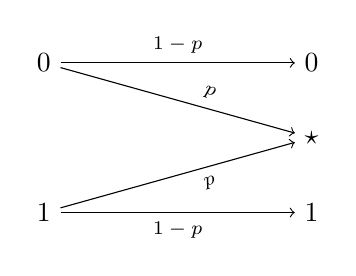
\begin{tikzpicture}[x=1cm,y=1cm]
		\node (i0) at (0,0.95)  {$0$};
		\node (i1) at (0,-0.95) {$1$};
		\node (o0) at (3.4,0.95)  {$0$};
		\node (os) at (3.4,0)    {$\star$};
		\node (o1) at (3.4,-0.95) {$1$};
		\draw[->,thin] (i0) -- node[above,font=\scriptsize] {$1-p$} (o0);
		\draw[->,thin] (i1) -- node[below,font=\scriptsize] {$1-p$} (o1);
		\draw[->,thin] (i0) -- node[pos=0.62,above,font=\scriptsize,sloped] {$p$} (os);
		\draw[->,thin] (i1) -- node[pos=0.62,below,font=\scriptsize,sloped] {$p$} (os);
	\end{tikzpicture}
	\end{center}
\end{example}

To use a channel $n$ times we pass to the \vocab{$n$th extension}, whose input alphabet is $\Ac^n$, whose output alphabet is $\Bc^n$, and whose channel matrix (for a DMC) is
$$\PP(y_1 \dots y_n \mid x_1 \dots x_n) = \prod_{i=1}^n \PP(y_i \mid x_i).$$

\begin{definition}[Code, Rate, Error Rate]
	A \vocab{code} $C$ of length $n$ is a function $\Mc \to \Ac^n$, where $\Mc$ is a set of messages; implicitly we also fix a decoding rule $\Bc^n \to \Mc$. We usually identify $C$ with its image, a subset of $\Ac^n$.
	\begin{itemize}
		\item The \vocab{size} of $C$ is $m = \abs{\Mc}$.
		\item The \vocab{information rate} of $C$ is $\rho(C) = \frac{1}{n}\log_2 m$.
		\item The \vocab{error rate} of $C$ is $\hat e(C) = \max_{x \in \Mc} \PP(\text{error} \mid x \text{ sent})$.
	\end{itemize}
\end{definition}

Throughout these notes $\log$ means $\log_2$ unless we say otherwise; this is the convention that makes the answers come out in bits.

\begin{definition}[Capacity]
	A channel can \vocab{transmit reliably at rate $R$} if there is a sequence of codes $(C_n)_{n \ge 1}$, with $C_n$ of length $n$, such that
	$$\lim_{n \to \infty} \rho(C_n) = R \qquad \text{and} \qquad \lim_{n \to \infty} \hat e(C_n) = 0.$$
	The \vocab{capacity} of the channel is the supremum of all rates at which it can transmit reliably.
\end{definition}

Note carefully what is being asked. We are not asking for one good code; we are asking for a whole family of codes whose rate stays bounded away from zero while the error probability is driven to zero. It is far from obvious that this can be done at all for a channel that makes errors, and the fact that it can -- that the binary symmetric channel with $p< \tfrac12$ has strictly positive capacity -- is Shannon's noisy coding theorem, which we prove in Section~\ref{sec:noisycoding}.

\section{Noiseless Coding}

We begin with the easier half of the problem, in which the channel is perfect and the only question is economy. A source emits symbols from an alphabet $\Ac$, some more often than others, and we want to represent them as short strings over a transmission alphabet $\Bc$.

\subsection{Codes and Decipherability}

Let $\Bc$ be a finite alphabet. Write $\Bc^\star = \bigcup_{n \ge 0} \Bc^n$ for the set of all finite strings over $\Bc$, including the empty string. The \vocab{concatenation} of $x = x_1 \dots x_r$ and $y = y_1 \dots y_s$ is $xy = x_1 \dots x_r y_1 \dots y_s$.

\begin{definition}[Code]
	Let $\Ac$ and $\Bc$ be alphabets. A \vocab{code} is a function $c \colon \Ac \to \Bc^\star$. The elements of the image of $c$ are the \vocab{codewords}.
\end{definition}

We write $m = \abs{\Ac}$ and $a = \abs{\Bc}$, and call $c$ an \vocab{$a$-ary code of size $m$}. A $2$-ary code is \emph{binary}, a $3$-ary code is \emph{ternary}.

\begin{example}[The Greek Fire Code]
	Take $\Ac = \{\alpha, \beta, \dots, \omega\}$, the $24$ letters of the Greek alphabet, and $\Bc = \{1,2,3,4,5\}$. Arrange the letters in a $5 \times 5$ square and encode each by its coordinates, so $c(\alpha) = 11$, $c(\beta) = 12$, and so on. To transmit the pair $xy$ one holds up $x$ torches on one hilltop and $y$ torches on another. This scheme is described by Polybius, and is very probably the oldest code in these notes by some two thousand years.
\end{example}

A code is only useful if we can send more than one symbol. Given a message $x_1 x_2 \dots x_n \in \Ac^\star$ we transmit $c(x_1)c(x_2)\dots c(x_n)$, so that $c$ extends to a map
$$c^\star \colon \Ac^\star \to \Bc^\star.$$

\begin{definition}[Decipherable]
	A code $c$ is \vocab{decipherable}, or \vocab{uniquely decodable}, if $c^\star$ is injective.
\end{definition}

It is not enough for $c$ itself to be injective, as the following shows.

\begin{example}
	Let $\Ac = \{1,2,3,4\}$ and $\Bc = \{0,1\}$, and set
	$$c(1) = 0, \quad c(2) = 1, \quad c(3) = 00, \quad c(4) = 01.$$
	This is injective, but $c^\star(114) = 0\,0\,01 = 0001$ and $c^\star(312) = 00\,0\,1 = 0001$, so $c^\star$ is not. On receiving $0001$ Bob has no way to tell which message was meant.
\end{example}

There are three easy ways of guaranteeing decipherability, assuming $c$ injective.

\begin{enumerate}[label=(\roman*)]
	\item A \vocab{block code}, in which all codewords have the same length. The Greek fire code is of this kind.
	\item A \vocab{comma code}, which reserves one letter of $\Bc$ to mark the end of a codeword and never uses it otherwise.
	\item A \vocab{prefix-free code}, in which no codeword is an initial segment of another.
\end{enumerate}

Block codes and comma codes are both special cases of prefix-free codes. Prefix-free codes have the pleasant property that Bob can decode as he reads: the moment the symbols he has seen form a codeword, he knows that codeword has ended, because no longer codeword begins that way. For this reason they are also called \vocab{instantaneous} codes.

Not every decipherable code is prefix-free. For instance $c(1) = 0$, $c(2) = 01$, $c(3) = 011$, $c(4) = 0111$ is decipherable -- each $0$ marks the start of a new codeword -- but $c(1)$ is a prefix of $c(2)$. Here Bob must look ahead to the next $0$ before committing. Remarkably, we shall see in a moment that allowing such lookahead buys us precisely nothing.

The right way to picture a prefix-free binary code is as a rooted binary tree. Reading a codeword left to right tells us which way to turn at each vertex, and the prefix-free condition says exactly that all the codewords sit at \emph{leaves}.

\begin{center}
\begin{tikzpicture}[x=1cm,y=1cm]
	\tikzset{dot/.style={circle, fill=black, inner sep=1.1pt}}
	\node[dot] (r)   at (0,0)      {};
	\node[dot] (l0)  at (-1.5,-1)  {};
	\node[dot] (n1)  at (1.5,-1)   {};
	\node[dot] (l10) at (0.4,-2)   {};
	\node[dot] (n11) at (2.6,-2)   {};
	\node[dot] (l110) at (1.7,-3)  {};
	\node[dot] (l111) at (3.5,-3)  {};
	\draw[thin] (r) -- node[above left,font=\scriptsize] {$0$} (l0);
	\draw[thin] (r) -- node[above right,font=\scriptsize] {$1$} (n1);
	\draw[thin] (n1) -- node[above left,font=\scriptsize] {$0$} (l10);
	\draw[thin] (n1) -- node[above right,font=\scriptsize] {$1$} (n11);
	\draw[thin] (n11) -- node[above left,font=\scriptsize] {$0$} (l110);
	\draw[thin] (n11) -- node[above right,font=\scriptsize] {$1$} (l111);
	\node[font=\small] at (-1.5,-1.42) {$0$};
	\node[font=\small] at (0.4,-2.42) {$10$};
	\node[font=\small] at (1.7,-3.42) {$110$};
	\node[font=\small] at (3.5,-3.42) {$111$};
\end{tikzpicture}
\end{center}

\subsection{Kraft's Inequality}

How short can the codewords of a prefix-free code be? Not arbitrarily short: the tree picture makes it clear that a short codeword uses up a lot of the tree. The following inequality measures exactly how much.

\begin{definition}[Kraft's Inequality]
	Let $c \colon \Ac \to \Bc^\star$ be a code with $\abs{\Ac} = m$ and $\abs{\Bc} = a$, whose codewords have lengths $\ell_1, \dots, \ell_m$. We say that $c$ satisfies \vocab{Kraft's inequality} if
	$$\sum_{i=1}^m a^{-\ell_i} \le 1.$$
\end{definition}

\begin{theorem}[Kraft]
	Given lengths $\ell_1, \dots, \ell_m$, there is a prefix-free $a$-ary code with these codeword lengths if and only if Kraft's inequality holds.
\end{theorem}

\begin{proof}
	Let $s = \max_i \ell_i$ and let $n_\ell$ be the number of $i$ with $\ell_i = \ell$, so that Kraft's inequality reads $\sum_{\ell=1}^s n_\ell a^{-\ell} \le 1$, or after multiplying by $a^s$,
	\begin{equation*} n_1 a^{s-1} + n_2 a^{s-2} + \dots + n_{s-1}a + n_s \le a^s. \tag{$\ast$}\end{equation*}

	Suppose first that $c$ is prefix-free. A codeword of length $\ell$ is a prefix of exactly $a^{s-\ell}$ strings of length $s$, and by the prefix-free condition no string of length $s$ has two different codewords as prefixes. So the left hand side of $(\ast)$ counts, without repetition, some of the strings of length $s$, of which there are $a^s$ in all. Hence $(\ast)$ holds.

	Conversely suppose $(\ast)$ holds; we build a prefix-free code with $n_\ell$ codewords of length $\ell$ for each $\ell$, by induction on $s$. If $s = 1$ the inequality says $n_1 \le a$ and we simply choose $n_1$ of the $a$ letters. For $s > 1$, the inductive hypothesis applied to the lengths at most $s-1$ gives a prefix-free code $\hat c$ with $n_\ell$ codewords of length $\ell$ for every $\ell < s$. Now the strings of length $s$ having some codeword of $\hat c$ as a prefix number exactly
	$$n_1 a^{s-1} + \dots + n_{s-1}a,$$
	so by $(\ast)$ at least $n_s$ strings of length $s$ remain untouched. Choosing $n_s$ of them and adjoining them to $\hat c$ gives a code which is still prefix-free, since none of the new codewords extends an old one (they were chosen to avoid this) and none of the old codewords extends a new one (they are shorter).
\end{proof}

\begin{remark}
	The proof is constructive, and gives a perfectly practical algorithm: list the required lengths in increasing order and greedily assign codewords, at each stage taking any string of the right length that does not extend a codeword already chosen. Kraft's inequality guarantees that we never run out.
\end{remark}

\subsection{McMillan's Inequality}

Now we come to the result promised above, which says that lookahead is worthless.

\begin{theorem}[McMillan]
	Every decipherable code satisfies Kraft's inequality.
\end{theorem}

\begin{proof}
	Let $c \colon \Ac \to \Bc^\star$ be decipherable with word lengths $\ell_1, \dots, \ell_m$, and set $s = \max_i \ell_i$. The trick is to consider the $R$th power of the quantity in question. For any $R \in \N$,
	$$\left(\sum_{i=1}^m a^{-\ell_i}\right)^{\!R} = \sum_{\ell=R}^{Rs} b_\ell\, a^{-\ell},$$
	where $b_\ell$ is the number of ways of choosing an ordered $R$-tuple of codewords whose total length is $\ell$; this is just what happens when we expand the product. Now a tuple of $R$ codewords of total length $\ell$ concatenates to a string in $\Bc^\ell$, and because $c$ is decipherable, distinct tuples give distinct strings. Hence
	$$b_\ell \le \abs{\Bc^\ell} = a^\ell,$$
	and so each term $b_\ell a^{-\ell}$ is at most $1$. There are at most $Rs$ terms, so
	$$\left(\sum_{i=1}^m a^{-\ell_i}\right)^{\!R} \le Rs, \qquad \text{that is} \qquad \sum_{i=1}^m a^{-\ell_i} \le (Rs)^{1/R}.$$
	Letting $R \to \infty$, the right hand side tends to $1$, and Kraft's inequality follows.
\end{proof}

The proof is a small piece of magic: an inequality that fails to hold is amplified by exponentiation into an absurdity, while the polynomial factor $Rs$ is powerless to keep up.

\begin{corollary}
	A decipherable code with word lengths $\ell_1, \dots, \ell_m$ exists if and only if a prefix-free code with the same word lengths exists.
\end{corollary}

\begin{proof}
	A prefix-free code is decipherable. Conversely, a decipherable code satisfies Kraft's inequality by McMillan, and then Kraft's theorem produces a prefix-free code with the same lengths.
\end{proof}

So from the point of view of word lengths -- which is the only point of view that matters for economy -- we may as well restrict attention to prefix-free codes, and we shall.

\subsection{Entropy}

We now need a way of saying how much information a source actually produces, so that we know what we are aiming at. The right notion is Shannon's \vocab{entropy}. Informally, the entropy of a random variable $X$ is the expected number of fair coin tosses needed to determine its value.

\begin{example}
	Suppose $X$ takes four values with probability $\tfrac14$ each. Identifying the values with $00, 01, 10, 11$, two coin tosses always suffice and never fewer, so the entropy should be $2$.

	Suppose instead $X$ takes four values with probabilities $\tfrac12, \tfrac14, \tfrac18, \tfrac18$. Identify them with the strings $0, 10, 110, 111$: toss a coin, and if it comes up $0$ we are done, otherwise toss again, and so on. The expected number of tosses is
	$$\tfrac12 \cdot 1 + \tfrac14 \cdot 2 + \tfrac18 \cdot 3 + \tfrac18 \cdot 3 = \tfrac74.$$
	The second variable is in this sense less random than the first.
\end{example}

Both examples are instances of the following.

\begin{definition}[Entropy]
	Let $X$ be a random variable taking finitely many values $x_1, \dots, x_n$ with probabilities $p_1, \dots, p_n$. The \vocab{entropy} of $X$ is
	$$H(X) = H(p_1, \dots, p_n) = -\sum_{i=1}^n p_i \log p_i = \EE[-\log p(X)],$$
	where $\log = \log_2$ and we adopt the convention $0\log 0 = 0$.
\end{definition}

The convention is forced on us by continuity, since $x \log x \to 0$ as $x \to 0^+$. Entropy is measured in \vocab{bits}. Clearly $H(X) \ge 0$, with equality if and only if some $p_i = 1$, that is, if and only if $X$ is constant.

\begin{example}[The Binary Entropy Function]
	For a biased coin with probability $p$ of heads we write
	$$H(p) = H(p, 1-p) = -p\log p - (1-p)\log(1-p).$$
	Differentiating, $H'(p) = \log\frac{1-p}{p}$, which is positive for $p< \tfrac12$ and negative for $p > \tfrac12$; and $H''(p) < 0$ throughout, so $H$ is strictly concave with a maximum of $1$ at $p = \tfrac12$, vanishing at $p=0$ and $p=1$.

	\begin{center}
	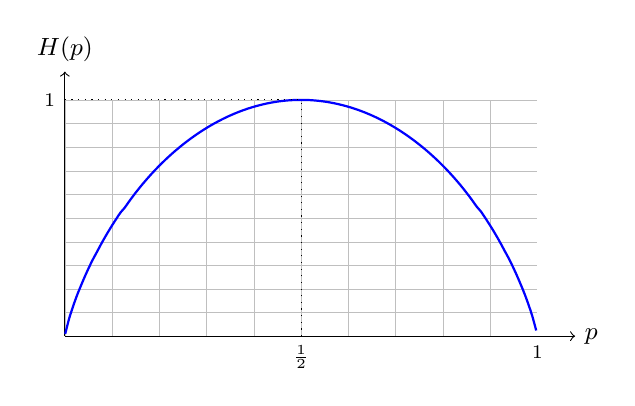
\begin{tikzpicture}[x=6cm,y=3cm]
		\draw[ultra thin,color=lightgray] (0,0) grid[xstep=0.1,ystep=0.1] (1,1);
		\draw[->,thin] (0,0) -- (1.08,0) node[right,font=\small] {$p$};
		\draw[->,thin] (0,0) -- (0,1.12) node[above,font=\small] {$H(p)$};
		\draw[thick,color=blue,smooth,samples=120,domain=0.0008:0.9992]
			plot (\x, {-(\x*ln(\x) + (1-\x)*ln(1-\x))/ln(2)});
		\draw[thin,dotted] (0.5,0) -- (0.5,1);
		\draw[thin,dotted] (0,1) -- (0.5,1);
		\node[font=\scriptsize,below] at (0.5,0) {$\frac12$};
		\node[font=\scriptsize,below] at (1,0) {$1$};
		\node[font=\scriptsize,left] at (0,1) {$1$};
	\end{tikzpicture}
	\end{center}

	This little function is going to appear everywhere, so it is worth committing its shape to memory: symmetric about $\tfrac12$, with infinite slope at the two ends.
\end{example}

The following inequality is the workhorse of the whole subject.

\begin{proposition}[Gibbs' Inequality]
	Let $(p_1, \dots, p_n)$ and $(q_1, \dots, q_n)$ be probability distributions. Then
	$$-\sum_{i=1}^n p_i \log p_i \le -\sum_{i=1}^n p_i \log q_i,$$
	with equality if and only if $p_i = q_i$ for all $i$.
\end{proposition}

The right hand side is the \vocab{cross entropy} of $q$ relative to $p$; the difference between the two sides is called the relative entropy, or Kullback--Leibler divergence, and Gibbs' inequality says it is non-negative.

\begin{proof}
	Since $\log x = \ln x/\ln 2$ we may work with natural logarithms throughout. Let $I = \{i : p_i \ne 0\}$. The elementary inequality $\ln x \le x-1$ for $x > 0$, with equality only at $x=1$, gives for $i \in I$
	$$\ln \frac{q_i}{p_i} \le \frac{q_i}{p_i} - 1,$$
	and multiplying by $p_i > 0$ and summing over $I$,
	$$\sum_{i \in I} p_i \ln \frac{q_i}{p_i} \le \sum_{i \in I} q_i - \sum_{i \in I} p_i \le 1 - 1 = 0,$$
	using $\sum_{i \in I} p_i = 1$ and $\sum_{i \in I} q_i \le 1$. Therefore
	$$-\sum_{i=1}^n p_i \ln p_i = -\sum_{i \in I} p_i \ln p_i \le -\sum_{i \in I} p_i \ln q_i \le -\sum_{i=1}^n p_i \ln q_i,$$
	the last step because the omitted terms have $p_i = 0$. If equality holds throughout we need $\sum_{i \in I} q_i = 1$ and $q_i/p_i = 1$ for every $i \in I$; the first forces $q_i = 0$ for $i \notin I$, and the second gives $p_i = q_i$ on $I$.
\end{proof}

\begin{corollary}
	$H(p_1, \dots, p_n) \le \log n$, with equality if and only if $p_1 = \dots = p_n = \frac1n$.
\end{corollary}

\begin{proof}
	Take $q_i = \frac1n$ in Gibbs' inequality: the right hand side is $-\sum p_i \log \frac1n = \log n$.
\end{proof}

In other words, the uniform distribution is the most random one, which is what one would hope.

\subsection{Optimal Codes and the Noiseless Coding Theorem}

Fix an alphabet $\Ac = \{\mu_1, \dots, \mu_m\}$ of $m \ge 2$ messages and a transmission alphabet $\Bc$ with $a = \abs{\Bc} \ge 2$. Let $X$ be a random variable on $\Ac$ with $\PP(X = \mu_i) = p_i$. A code $c$ with word lengths $\ell_1, \dots, \ell_m$ has expected word length
$$\EE[S] = \sum_{i=1}^m p_i \ell_i.$$

\begin{definition}[Optimal Code]
	A code $c \colon \Ac \to \Bc^\star$ is \vocab{optimal} if it has the smallest expected word length among all decipherable codes for $X$.
\end{definition}

We can now say precisely how well one can do.

\begin{theorem}[Shannon's Noiseless Coding Theorem]\label{thm:noiseless}
	The expected word length $\EE[S]$ of an optimal code satisfies
	$$\frac{H(X)}{\log a} \le \EE[S] < \frac{H(X)}{\log a} + 1.$$
	Moreover the lower bound holds for \emph{every} decipherable code, and is attained exactly when $p_i = a^{-\ell_i}$ for integers $\ell_i$ (so that in particular $\sum_i a^{-\ell_i} = 1$).
\end{theorem}

\begin{proof}
	\emph{The lower bound.} Let $c$ be an arbitrary decipherable code, with word lengths $\ell_1, \dots, \ell_m$. Put $D = \sum_i a^{-\ell_i}$ and $q_i = a^{-\ell_i}/D$, so that $(q_i)$ is a probability distribution. By Gibbs' inequality,
	\begin{align*}
		H(X) \ \le\  -\sum_i p_i \log q_i &= -\sum_i p_i\left(-\ell_i \log a - \log D\right)\\
		&= \log D + \log a \sum_i p_i \ell_i.
	\end{align*}
	By McMillan's inequality $D \le 1$, so $\log D \le 0$, and therefore
	$$H(X) \le \log a \cdot \EE[S],$$
	which is the lower bound. Equality forces $D = 1$ and $p_i = q_i = a^{-\ell_i}$.

	\emph{The upper bound.} It suffices to exhibit \emph{some} decipherable code beating the bound, since an optimal code can only be better. Set
	$$\ell_i = \ceil{-\log_a p_i},$$
	so that $-\log_a p_i \le \ell_i < -\log_a p_i + 1$. From the first inequality $p_i \ge a^{-\ell_i}$, and summing, $\sum_i a^{-\ell_i} \le 1$. So Kraft's inequality holds and there is a prefix-free code $c$ with these word lengths. From the second inequality,
	$$\EE[S] = \sum_i p_i \ell_i < \sum_i p_i \left(-\log_a p_i + 1\right) = \frac{H(X)}{\log a} + 1. \qedhere$$
\end{proof}

The code constructed in the second half is worth a name.

\begin{definition}[Shannon--Fano Coding]
	The \vocab{Shannon--Fano code} for probabilities $p_1, \dots, p_m$ takes word lengths $\ell_i = \ceil{-\log_a p_i}$ and then assigns codewords greedily in order of increasing length, as in the proof of Kraft's theorem.
\end{definition}

\begin{example}\label{ex:shannonfano}
	Take $a = 2$ and the source
	$$\begin{array}{c|cccccc}
		i & 1 & 2 & 3 & 4 & 5 & 6 \\ \hline
		p_i & 0.30 & 0.22 & 0.18 & 0.14 & 0.10 & 0.06
	\end{array}$$
	The entropy is
	$$H(X) = -\sum_i p_i \log p_i \approx 2.4198.$$
	The Shannon--Fano lengths are $\ell_i = \ceil{-\log_2 p_i}$, namely
	$$\ell = (2,3,3,3,4,5),$$
	and $\sum_i 2^{-\ell_i} = \tfrac14 + 3\cdot\tfrac18 + \tfrac1{16}+\tfrac1{32} = 0.71875 \le 1$ as it must be. Assigning codewords greedily gives
	$$\begin{array}{c|cccccc}
		i & 1 & 2 & 3 & 4 & 5 & 6 \\ \hline
		c(i) & 00 & 010 & 011 & 100 & 1010 & 10110
	\end{array}$$
	with expected word length
	$$\EE[S] = 0.30\cdot 2 + 0.22 \cdot 3 + 0.18 \cdot 3 + 0.14\cdot 3 + 0.10\cdot 4 + 0.06\cdot 5 = 2.92.$$
	This does obey $H(X) \le \EE[S] < H(X)+1$, but only just, and it is visibly wasteful: nothing at all uses the string $11$, and we could shorten $c(6)$ to $1011$ without breaking anything. Shannon--Fano coding is not optimal.
\end{example}

\subsection{Huffman Coding}

Huffman's algorithm produces a genuinely optimal code, and it does so by a beautifully simple greedy rule. We take $a = 2$ and $\Bc = \{0,1\}$ for simplicity; everything generalises.

Order the messages so that $p_1 \ge p_2 \ge \dots \ge p_m$. We define the code recursively.

\begin{definition}[Huffman Code]
	If $m = 2$, take the codewords $0$ and $1$. If $m > 2$, form the source on $m-1$ symbols $\mu_1, \dots, \mu_{m-2}, \nu$ with probabilities $p_1, \dots, p_{m-2}, p_{m-1}+p_m$, take a \vocab{Huffman code} for it, and then set
	$$c(\mu_{m-1}) = c(\nu)0, \qquad c(\mu_m) = c(\nu)1,$$
	keeping all other codewords unchanged.
\end{definition}

In other words: repeatedly merge the two least likely symbols into one, until only two remain; then read the resulting binary tree from the root outwards. Huffman codes are prefix-free by construction, since every codeword sits at a leaf. They are not unique -- ties in the probabilities force arbitrary choices -- but we shall see that all the choices are equally good.

\begin{example}\label{ex:huffman}
	Take the same source as Example~\ref{ex:shannonfano}, writing the messages as $A, \dots, F$:
	$$\begin{array}{c|cccccc}
		 & A & B & C & D & E & F \\ \hline
		p & 0.30 & 0.22 & 0.18 & 0.14 & 0.10 & 0.06
	\end{array}$$
	We merge repeatedly.
	\begin{itemize}
		\item The two smallest are $E$ and $F$; merge them into $X$ with probability $0.16$. Remaining: $A\,0.30$, $B\,0.22$, $C\,0.18$, $X\,0.16$, $D\,0.14$.
		\item The two smallest are $D$ and $X$; merge them into $Y$ with probability $0.30$. Remaining: $A\,0.30$, $Y\,0.30$, $B\,0.22$, $C\,0.18$.
		\item The two smallest are $C$ and $B$; merge them into $Z$ with probability $0.40$. Remaining: $A\,0.30$, $Y\,0.30$, $Z\,0.40$.
		\item The two smallest are $A$ and $Y$; merge them into $W$ with probability $0.60$.
		\item Finally merge $Z$ and $W$.
	\end{itemize}
	The resulting tree is as follows, with $0$ on the left branch and $1$ on the right.

	\begin{center}
	\begin{tikzpicture}[x=1cm,y=1.15cm]
		\tikzset{dot/.style={circle, fill=black, inner sep=1.1pt}}
		\node[dot,label={[font=\scriptsize]above:$1.00$}] (rt) at (0,0) {};
		\node[dot,label={[font=\scriptsize]above left:$0.40$}] (Zn) at (-2.6,-1) {};
		\node[dot,label={[font=\scriptsize]above right:$0.60$}] (Wn) at (1.6,-1) {};
		\node (B) at (-3.7,-2) {$B$};
		\node (C) at (-1.5,-2) {$C$};
		\node (A) at (0.3,-2) {$A$};
		\node[dot,label={[font=\scriptsize]above right:$0.30$}] (Yn) at (2.9,-2) {};
		\node (D) at (1.9,-3) {$D$};
		\node[dot,label={[font=\scriptsize]above right:$0.16$}] (Xn) at (3.9,-3) {};
		\node (E) at (3.1,-4) {$E$};
		\node (F) at (4.7,-4) {$F$};
		\draw[thin] (rt) -- node[above left,font=\scriptsize] {$0$} (Zn);
		\draw[thin] (rt) -- node[above right,font=\scriptsize] {$1$} (Wn);
		\draw[thin] (Zn) -- node[above left,font=\scriptsize] {$0$} (B);
		\draw[thin] (Zn) -- node[above right,font=\scriptsize] {$1$} (C);
		\draw[thin] (Wn) -- node[above left,font=\scriptsize] {$0$} (A);
		\draw[thin] (Wn) -- node[above right,font=\scriptsize] {$1$} (Yn);
		\draw[thin] (Yn) -- node[above left,font=\scriptsize] {$0$} (D);
		\draw[thin] (Yn) -- node[above right,font=\scriptsize] {$1$} (Xn);
		\draw[thin] (Xn) -- node[above left,font=\scriptsize] {$0$} (E);
		\draw[thin] (Xn) -- node[above right,font=\scriptsize] {$1$} (F);
		\node[font=\scriptsize] at (-3.7,-2.45) {$00$};
		\node[font=\scriptsize] at (-1.5,-2.45) {$01$};
		\node[font=\scriptsize] at (0.3,-2.45) {$10$};
		\node[font=\scriptsize] at (1.9,-3.45) {$110$};
		\node[font=\scriptsize] at (3.1,-4.45) {$1110$};
		\node[font=\scriptsize] at (4.7,-4.45) {$1111$};
	\end{tikzpicture}
	\end{center}

	Reading off, the word lengths are $2,2,2,3,4,4$ and
	$$\EE[S] = 0.30\cdot2 + 0.22\cdot2+0.18\cdot2+0.14\cdot3+0.10\cdot4+0.06\cdot4 = 2.46,$$
	comfortably better than the $2.92$ of Shannon--Fano, and within $0.05$ of the entropy bound $2.4198$.
\end{example}

To prove optimality we need two structural facts about optimal codes, both of which are obvious once stated.

\begin{lemma}\label{lem:optprops}
	Let $c$ be an optimal prefix-free code for messages $\mu_1, \dots, \mu_m$ with probabilities $p_1 \ge \dots \ge p_m$, and word lengths $\ell_1, \dots, \ell_m$. Then
	\begin{enumerate}[label=(\roman*)]
		\item if $p_i > p_j$ then $\ell_i \le \ell_j$;
		\item among the codewords of maximal length, there are two which differ only in their last digit.
	\end{enumerate}
\end{lemma}

\begin{proof}
	\emph{(i).} Suppose $p_i > p_j$ but $\ell_i > \ell_j$. Swapping the $i$th and $j$th codewords leaves the code prefix-free and changes the expected word length by
	$$(p_i \ell_j + p_j \ell_i) - (p_i \ell_i + p_j \ell_j) = (p_i - p_j)(\ell_j - \ell_i) < 0,$$
	contradicting optimality.

	\emph{(ii).} Let $\ell = \max_i \ell_i$, and suppose no two codewords of length $\ell$ agree in their first $\ell - 1$ digits. Deleting the final digit of every codeword of length $\ell$ then leaves all these codewords distinct; and the code is still prefix-free, because a shortened codeword $y$ could only be a prefix of some other codeword $z$ if $y0$ or $y1$ were, and $z$ has length at most $\ell$, so $z \in \{y0, y1\}$, which our assumption excludes. But this strictly decreases the expected word length, contradicting optimality.
\end{proof}

\begin{theorem}
	Huffman codes are optimal.
\end{theorem}

\begin{proof}
	We induct on $m$. For $m = 2$ the Huffman code has both word lengths equal to $1$, which is clearly best possible.

	Let $m > 2$ and let $c_m$ be the Huffman code for $X_m$ taking values $\mu_1, \dots, \mu_m$ with probabilities $p_1 \ge \dots \ge p_m$. By construction $c_m$ is built from a Huffman code $c_{m-1}$ for the merged source $X_{m-1}$ on $\mu_1, \dots, \mu_{m-2}, \nu$ with probabilities $p_1, \dots, p_{m-2}, p_{m-1}+p_m$, by extending the codeword of $\nu$ by one digit in each of two ways. Comparing expected lengths term by term,
	\begin{equation*}\EE[S_m] = \EE[S_{m-1}] + p_{m-1} + p_m. \tag{1}\end{equation*}

	Now let $c_m'$ be an optimal code for $X_m$; by the corollary to McMillan's theorem we may take it prefix-free. By Lemma~\ref{lem:optprops}(i) the two longest codewords belong to two of the least likely messages, and by (ii) we may assume, after relabelling messages of equal probability and swapping codewords of equal length, that
	$$c_m'(\mu_{m-1}) = y0, \qquad c_m'(\mu_m) = y1$$
	for some string $y$. Define a code $c_{m-1}'$ for $X_{m-1}$ by
	$$c_{m-1}'(\mu_i) = c_m'(\mu_i) \ (i \le m-2), \qquad c_{m-1}'(\nu) = y.$$
	This is prefix-free: no codeword of $c_m'$ other than $y0, y1$ can have $y$ as a prefix, else it would have $y0$ or $y1$ as a prefix. Exactly as in (1),
	\begin{equation*}\EE[S_m'] = \EE[S_{m-1}'] + p_{m-1} + p_m. \tag{2}\end{equation*}
	By the inductive hypothesis $c_{m-1}$ is optimal for $X_{m-1}$, so $\EE[S_{m-1}] \le \EE[S_{m-1}']$. Combining with (1) and (2),
	$$\EE[S_m] \le \EE[S_m'],$$
	and since $c_m'$ was optimal, so is $c_m$.
\end{proof}

\begin{remark}
	Not every optimal code is a Huffman code -- one can always relabel $0 \leftrightarrow 1$ in a subtree, for instance. What the theorem really gives us is that the Huffman word lengths are optimal word lengths.

	Huffman coding is optimal but not perfect: it can never do better than the entropy bound, and if one symbol has probability close to $1$ it must still spend a whole bit on it. The remedy is to Huffman-code blocks of $N$ symbols at a time, which as we shall see in Section~\ref{sec:infotheory} drives the cost per symbol down to the entropy.
\end{remark}

\subsection{Joint Entropy}

Finally in this section we record how entropy behaves for pairs of random variables, which we shall need repeatedly later on.

If $X, Y$ take values in $\Ac, \Bc$ then $(X,Y)$ takes values in $\Ac \times \Bc$, and its entropy
$$H(X,Y) = -\sum_{x \in \Ac}\sum_{y \in \Bc} \PP(X = x, Y=y)\log \PP(X=x,Y=y)$$
is called the \vocab{joint entropy}. The same definition works for any finite tuple.

\begin{lemma}[Subadditivity]\label{lem:subadd}
	$H(X,Y) \le H(X) + H(Y)$, with equality if and only if $X$ and $Y$ are independent.
\end{lemma}

\begin{proof}
	Write $\Ac = \{x_1, \dots, x_m\}$, $\Bc = \{y_1, \dots, y_n\}$, and set $p_{ij} = \PP(X = x_i, Y = y_j)$, $p_i = \PP(X = x_i)$, $q_j = \PP(Y = y_j)$. Both $(p_{ij})$ and $(p_iq_j)$ are probability distributions on $\Ac \times \Bc$, so Gibbs' inequality applies and gives
	\begin{align*}
		H(X,Y) = -\sum_{i,j} p_{ij}\log p_{ij} &\le -\sum_{i,j}p_{ij}\log(p_iq_j) \\
		&= -\sum_i \Bigl(\sum_j p_{ij}\Bigr)\log p_i - \sum_j \Bigl(\sum_i p_{ij}\Bigr)\log q_j \\
		&= -\sum_i p_i \log p_i - \sum_j q_j \log q_j = H(X) + H(Y).
	\end{align*}
	Equality in Gibbs holds precisely when $p_{ij} = p_iq_j$ for all $i,j$, which is exactly independence.
\end{proof}

Intuitively: knowing two things at once is never harder than knowing each separately, and it is exactly as hard only when the two are unrelated.


\section{Noisy Channels and Error-Correcting Codes}

We now switch the channel back on. Throughout this section, unless we say otherwise, the channel is the binary symmetric channel with error probability $p < \tfrac12$, and a code is a subset of $\F_2^n$.

\begin{definition}[Binary Code]
	A \vocab{binary $[n,m]$-code} is a subset $C \subseteq \{0,1\}^n$ with $\abs{C} = m$. We call $n$ the \vocab{length} of the code and the elements of $C$ its \vocab{codewords}.
\end{definition}

Such a code lets us send one of $m$ messages using $n$ bits, that is, using the channel $n$ times. Since $1 \le m \le 2^n$, the information rate $\rho(C) = \frac1n \log m$ satisfies $0 \le \rho(C) \le 1$, with $\rho(C) = 0$ for the useless code $\abs{C} = 1$ and $\rho(C) = 1$ for the code $C = \{0,1\}^n$ which does no error correction at all. All the interest lies in between.

\subsection{Decoding Rules}

Suppose Bob receives $x \in \{0,1\}^n$. What should he guess was sent? There are three natural answers.

\begin{definition}[Decoding Rules]
	Let $C$ be a binary $[n,m]$-code.
	\begin{itemize}
		\item The \vocab{ideal observer} rule decodes $x$ as the codeword $c \in C$ maximising $\PP(c \text{ sent} \mid x \text{ received})$.
		\item The \vocab{maximum likelihood} rule decodes $x$ as the $c \in C$ maximising the probability $\PP(x \text{ received} \mid c \text{ sent})$.
		\item The \vocab{minimum distance} rule decodes $x$ as the $c \in C$ minimising the Hamming distance $d(x,c)$,
		$$d(x,y) = \abs{\{i : x_i \ne y_i\}}.$$
	\end{itemize}
\end{definition}

The first is what we actually want, but it requires knowing the prior distribution on messages. The third is what we can actually compute. Happily, under mild hypotheses they all coincide.

\begin{lemma}\label{lem:decoding}
	Let $C$ be a binary $[n,m]$-code used over a BSC with error probability $p$.
	\begin{enumerate}[label=(\roman*)]
		\item If all messages are equally likely, the ideal observer and maximum likelihood rules agree.
		\item If $p < \tfrac12$, the maximum likelihood and minimum distance rules agree.
	\end{enumerate}
\end{lemma}

\begin{proof}
	\emph{(i).} By Bayes' theorem,
	$$\PP(c \text{ sent} \mid x \text{ received}) = \frac{\PP(c \text{ sent})}{\PP(x \text{ received})}\,\PP(x \text{ received}\mid c \text{ sent}).$$
	For fixed $x$, the denominator does not depend on $c$, and by hypothesis neither does $\PP(c \text{ sent})$. So the two quantities are maximised together.

	\emph{(ii).} If $d(x,c) = r$ then exactly $r$ of the $n$ transmitted bits were flipped, so
	$$\PP(x \text{ received} \mid c \text{ sent}) = p^r(1-p)^{n-r} = (1-p)^n\left(\frac{p}{1-p}\right)^{\!r}.$$
	As $p < \tfrac12$ we have $\frac{p}{1-p} < 1$, so this is a strictly decreasing function of $r$. Maximising it is therefore the same as minimising $r = d(x,c)$.
\end{proof}

The hypothesis in (i) is reasonable in practice, because if we first compress the message using a good noiseless code the resulting bits look close to uniform. The hypothesis in (ii) is harmless, as discussed earlier. Channels with $p = 0$ are called \vocab{lossless}, and channels with $p = \tfrac12$ are called \vocab{useless}.

It is worth seeing that the rules really can differ.

\begin{example}
	Let $C = \{000, 111\}$, sent with probabilities $\alpha = \tfrac9{10}$ and $1-\alpha = \tfrac1{10}$ respectively, over a BSC with $p = \tfrac14$. Suppose $110$ is received. Then
	$$\PP(000 \text{ sent} \mid 110) = \frac{\alpha p^2(1-p)}{\alpha p^2 (1-p) + (1-\alpha)p(1-p)^2} = \frac{\tfrac9{10}\cdot \tfrac1{16}\cdot\tfrac34}{\tfrac9{10}\cdot\tfrac1{16}\cdot\tfrac34 + \tfrac1{10}\cdot\tfrac14\cdot\tfrac9{16}} = \frac34,$$
	so $\PP(111 \text{ sent} \mid 110) = \tfrac14$. The ideal observer decodes $110$ as $000$, since $000$ was so much more likely \emph{a priori}. But $d(110,111) = 1 < 2 = d(110,000)$, so minimum distance decoding -- and hence maximum likelihood decoding -- gives $111$.
\end{example}

\begin{remark}
	Minimum distance decoding is conceptually simple but potentially expensive: naively one compares the received word against every codeword, which is hopeless once $\abs{C}$ is large. Much of Section~\ref{sec:linear} is devoted to making it cheap for structured codes. One should also fix a convention for ties: either make an arbitrary choice, or declare a failure and ask for retransmission.
\end{remark}

From now on we use minimum distance decoding.

\subsection{Error Detection and Correction}

\begin{definition}
	A binary $[n,m]$-code $C$ is
	\begin{itemize}
		\item \vocab{$d$-error detecting} if changing at most $d$ digits of a codeword can never produce another codeword;
		\item \vocab{$e$-error correcting} if, knowing that $x \in \F_2^n$ differs from some codeword in at most $e$ places, we can determine that codeword.
	\end{itemize}
\end{definition}

\begin{example}[Repetition Code]
	The \vocab{repetition code} of length $n$ has codewords $00\dots0$ and $11\dots1$. It is an $[n,2]$-code, it is $(n-1)$-error detecting and $\floor{\frac{n-1}{2}}$-error correcting, and its information rate is $\frac1n$, which tends to $0$. Reliability is bought at the price of everything else.
\end{example}

\begin{example}[Simple Parity Check Code]
	The \vocab{simple parity check code} (or \vocab{paper tape code}) of length $n$ is
	$$C = \Bigl\{(x_1, \dots, x_n) \in \F_2^n : \sum_{i=1}^n x_i = 0\Bigr\}.$$
	This is an $[n, 2^{n-1}]$-code, it is $1$-error detecting and $0$-error correcting, and its information rate is $\frac{n-1}{n} \to 1$. Economy is bought at the price of everything else.
\end{example}

Between these two extremes sits the first genuinely clever code.

\begin{example}[Hamming's Original Code]\label{ex:ham74}
	Define $C \subseteq \F_2^7$ by the three conditions
	$$c_1 + c_3 + c_5 + c_7 = 0, \qquad c_2 + c_3 + c_6 + c_7 = 0, \qquad c_4 + c_5 + c_6 + c_7 = 0.$$
	The digits $c_3, c_5, c_6, c_7$ may be chosen freely and then $c_1, c_2, c_4$ are determined, so $\abs{C} = 2^4 = 16$ and $C$ is a $[7,16]$-code with rate $\frac47$.

	Suppose $x \in \F_2^7$ is received. Form the \vocab{syndrome} $z = (z_1, z_2, z_4)$ where
	$$z_1 = x_1+x_3+x_5+x_7, \quad z_2 = x_2+x_3+x_6+x_7, \quad z_4 = x_4+x_5+x_6+x_7.$$
	If $x \in C$ then $z = (0,0,0)$. If instead $x = c + e_i$, a codeword with the $i$th digit flipped, then by linearity $z_x = z_{e_i}$, and one checks case by case that
	$$z_1 + 2z_2 + 4z_4 = i$$
	as an ordinary integer. For instance $e_5$ appears in the first and third conditions but not the second, giving $z = (1,0,1)$ and $1 + 0 + 4 = 5$. So the syndrome does not merely tell us that an error has occurred, it tells us \emph{where}: the code is $1$-error correcting. This is a remarkably efficient piece of bookkeeping, and we will see in a moment that in a precise sense it cannot be improved on.
\end{example}

To analyse such codes properly we need the geometry of $\F_2^n$.

\begin{lemma}
	The Hamming distance $d$ is a metric on $\F_2^n$.
\end{lemma}

\begin{proof}
	Certainly $d(x,y) \ge 0$ with equality if and only if $x = y$, and $d(x,y) = d(y,x)$. For the triangle inequality, note that if $x_i \ne z_i$ then $x_i \ne y_i$ or $y_i \ne z_i$, so
	$$\{i : x_i \ne z_i\} \subseteq \{i : x_i \ne y_i\} \cup \{i : y_i \ne z_i\},$$
	and taking sizes gives $d(x,z) \le d(x,y) + d(y,z)$.
\end{proof}

Equivalently, $d(x,y) = \sum_i d_1(x_i,y_i)$ where $d_1$ is the discrete metric on $\F_2$; the triangle inequality is inherited coordinatewise.

\begin{definition}[Minimum Distance]
	The \vocab{minimum distance} of a code $C$ with $\abs{C} \ge 2$ is
	$$d(C) = \min\{d(c_1,c_2) : c_1, c_2 \in C, \, c_1 \ne c_2\}.$$
	An $[n,m]$-code with minimum distance $d$ is called an $[n,m,d]$-code.
\end{definition}

\begin{lemma}\label{lem:mindist}
	Let $C$ be a code with minimum distance $d$. Then
	\begin{enumerate}[label=(\roman*)]
		\item $C$ is $(d-1)$-error detecting, but cannot detect all sets of $d$ errors;
		\item $C$ is $\floor{\frac{d-1}{2}}$-error correcting, but cannot correct all sets of $\floor{\frac{d-1}{2}}+1$ errors.
	\end{enumerate}
\end{lemma}

\begin{proof}
	\emph{(i).} If $c \in C$ and $1 \le d(x,c) \le d-1$ then $x \notin C$, since every other codeword is at distance at least $d$ from $c$; so the corruption is detected. On the other hand if $c_1, c_2$ are codewords at distance exactly $d$, then $d$ well-chosen errors carry $c_1$ to $c_2$ and nothing at all is noticed.

	\emph{(ii).} Put $e = \floor{\frac{d-1}{2}}$, so that $2e < d$. Suppose $x \in \F_2^n$ and $c_1 \in C$ with $d(x,c_1) \le e$. For any other codeword $c_2$, the triangle inequality gives
	$$d(x,c_2) \ge d(c_1,c_2) - d(x,c_1) \ge d - e > e,$$
	so $c_1$ is the unique codeword within distance $e$ of $x$ and we recover it. For the second half, choose $c_1, c_2$ with $d(c_1,c_2) = d$ and let $x$ agree with $c_1$ except in $e+1$ of the places where $c_1$ and $c_2$ differ. Then $d(x,c_1) = e+1$ while $d(x,c_2) = d - (e+1) \le e+1$, using $d \le 2(e+1)$; so $x$ is at least as close to $c_2$ as to $c_1$ and we cannot reliably decode.
\end{proof}

\begin{example}
	The repetition code of length $n$ is an $[n,2,n]$-code. The simple parity check code of length $n$ is an $[n,2^{n-1},2]$-code, since flipping any two digits preserves the parity. The trivial code $\F_2^n$ is an $[n,2^n,1]$-code. Hamming's original code is $1$-error correcting so has $d \ge 3$ by Lemma~\ref{lem:mindist}; and $0000000$ and $1110000$ are both codewords, so $d = 3$ exactly, making it a $[7,16,3]$-code.
\end{example}

\subsection{Covering Estimates and Perfect Codes}

The picture behind Lemma~\ref{lem:mindist} is that an $e$-error correcting code is a packing of disjoint balls of radius $e$ into $\F_2^n$. Counting gives an immediate upper bound on how many codewords there can be.

\begin{definition}
	For $x \in \F_2^n$ and $r \ge 0$, write $B(x,r) = \{y \in \F_2^n : d(x,y) \le r\}$ for the closed \vocab{Hamming ball} of radius $r$. Its size does not depend on $x$, and we write
	$$V(n,r) = \abs{B(x,r)} = \sum_{i=0}^{r}\binom{n}{i}.$$
\end{definition}

\begin{center}
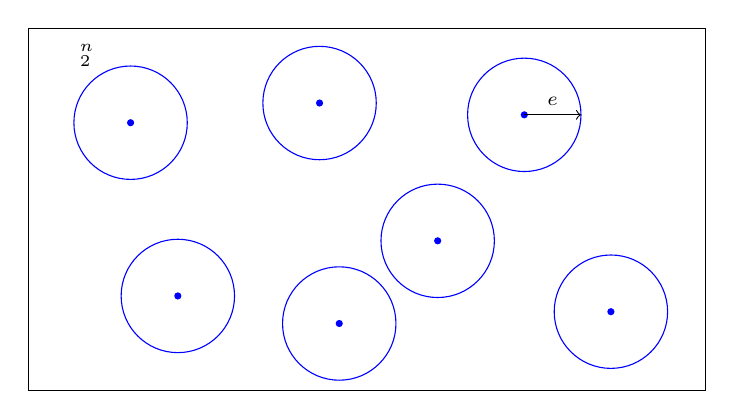
\begin{tikzpicture}[x=1cm,y=1cm]
	\draw[thin] (-4.3,-2.3) rectangle (4.3,2.3);
	\node[font=\small] at (-3.55,1.95) {$\F_2^n$};
	\foreach \pos in {(-3,1.1), (-0.6,1.35), (2,1.2), (-2.4,-1.1), (0.9,-0.4), (3.1,-1.3), (-0.35,-1.45)}{
		\draw[thin,color=blue] \pos circle (0.72);
		\fill[color=blue] \pos circle (1.3pt);
	}
	\draw[->,thin] (2,1.2) -- node[above,font=\scriptsize] {$e$} ++(0.72,0);
\end{tikzpicture}
\end{center}

The dots are the codewords; the discs are the balls of radius $e$ inside which minimum distance decoding succeeds. They must be disjoint, and they all live inside a space of size $2^n$.

\begin{lemma}[Hamming's Bound; the Sphere-Packing Bound]\label{lem:hamming}
	An $e$-error correcting code $C$ of length $n$ satisfies
	$$\abs{C} \le \frac{2^n}{V(n,e)}.$$
\end{lemma}

\begin{proof}
	If $c_1 \ne c_2$ are codewords then $B(c_1,e) \cap B(c_2,e) = \varnothing$, since a point in the intersection could not be decoded. Hence
	$$\sum_{c \in C} \abs{B(c,e)} \le \abs{\F_2^n}, \qquad \text{that is} \qquad \abs{C}\,V(n,e) \le 2^n. \qedhere$$
\end{proof}

\begin{definition}[Perfect Code]
	An $e$-error correcting code $C$ of length $n$ with $\abs{C} = \frac{2^n}{V(n,e)}$ is called \vocab{perfect}.
\end{definition}

\begin{remark}
	Equivalently, $C$ is perfect if the balls $B(c,e)$ for $c \in C$ partition $\F_2^n$: every word in the space is within distance $e$ of exactly one codeword. Perfect codes are wonderfully efficient but also brittle, since any $e+1$ errors are guaranteed to be decoded to the wrong codeword, with no warning.
\end{remark}

\begin{example}
	Hamming's $[7,16,3]$-code is $1$-error correcting, and
	$$\frac{2^7}{V(7,1)} = \frac{128}{1+7} = 16 = \abs{C},$$
	so it is perfect. Indeed, the syndrome map sends $\F_2^7$ onto $\F_2^3$, and the eight syndromes correspond precisely to `no error' and the seven possible single-bit errors.
\end{example}

\begin{example}
	The repetition code of length $n$ is perfect if and only if $n$ is odd. If $n = 2k+1$ it is $k$-error correcting and $V(n,k) = \sum_{i \le k}\binom{n}{i} = 2^{n-1}$ by symmetry, so $2^n/V(n,k) = 2 = \abs{C}$. If $n$ is even the count fails.
\end{example}

The smallest interesting case is worth drawing. Here is $\F_2^3$ as the vertices of a cube, with the repetition code $\{000,111\}$ marked.

\begin{center}
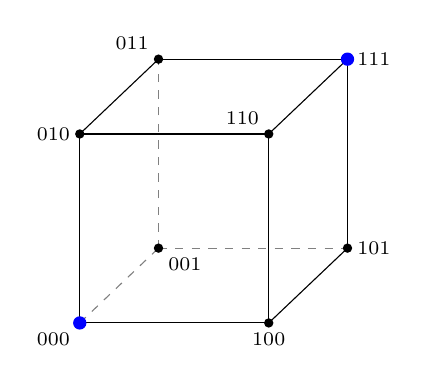
\begin{tikzpicture}[x=1cm,y=1cm]
	\tikzset{dot/.style={circle,fill=black,inner sep=1.2pt},
	         cod/.style={circle,fill=blue,inner sep=1.7pt}}
	\coordinate (v000) at (0,0);
	\coordinate (v100) at (2.4,0);
	\coordinate (v010) at (0,2.4);
	\coordinate (v110) at (2.4,2.4);
	\coordinate (v001) at (1,0.95);
	\coordinate (v101) at (3.4,0.95);
	\coordinate (v011) at (1,3.35);
	\coordinate (v111) at (3.4,3.35);
	\draw[thin] (v000)--(v100)--(v110)--(v010)--cycle;
	\draw[thin] (v101)--(v111)--(v011);
	\draw[thin] (v100)--(v101);
	\draw[thin] (v110)--(v111); \draw[thin] (v010)--(v011);
	\draw[thin,dashed,color=gray] (v001)--(v101);
	\draw[thin,dashed,color=gray] (v001)--(v011);
	\draw[thin,dashed,color=gray] (v000)--(v001);
	\node[cod] at (v000) {}; \node[cod] at (v111) {};
	\node[dot] at (v100) {}; \node[dot] at (v010) {};
	\node[dot] at (v110) {}; \node[dot] at (v001) {};
	\node[dot] at (v101) {}; \node[dot] at (v011) {};
	\node[font=\scriptsize,below left] at (v000) {$000$};
	\node[font=\scriptsize,below] at (v100) {$100$};
	\node[font=\scriptsize,left] at (v010) {$010$};
	\node[font=\scriptsize,above left] at (v110) {$110$};
	\node[font=\scriptsize,below right] at (v001) {$001$};
	\node[font=\scriptsize,right] at (v101) {$101$};
	\node[font=\scriptsize,above left] at (v011) {$011$};
	\node[font=\scriptsize,right] at (v111) {$111$};
\end{tikzpicture}
\end{center}

Every vertex is adjacent to exactly one of the two blue vertices, which is the statement that the $[3,2,3]$ repetition code is perfect.

\begin{remark}
	If $\frac{2^n}{V(n,e)}$ is not an integer then certainly no perfect $e$-error correcting code of length $n$ exists. The converse is false: with $n = 90$ and $e = 2$ the quotient is an integer, but no such code exists.
\end{remark}

\begin{definition}
	$A(n,d)$ denotes the largest $m$ for which an $[n,m,d]$-code exists.
\end{definition}

Determining $A(n,d)$ in general is a hard open problem, and only small cases are known.

\begin{example}
	$A(n,1) = 2^n$, achieved by the trivial code. $A(n,2) = 2^{n-1}$, achieved by the simple parity check code (the upper bound follows from the next theorem). $A(n,n) = 2$, achieved by the repetition code.
\end{example}

\begin{lemma}\label{lem:Amono}
	$A(n,d+1) \le A(n,d)$.
\end{lemma}

\begin{proof}
	Let $m = A(n,d+1)$ and let $C$ be an $[n,m,d+1]$-code. Choose distinct $c_1, c_2 \in C$ with $d(c_1,c_2) = d+1$, and let $c_1'$ differ from $c_1$ in exactly one of the places where $c_1$ and $c_2$ differ, so $d(c_1',c_2) = d$. For any other $c \in C$,
	$$d+1 \le d(c,c_1) \le d(c,c_1') + d(c_1',c_1) = d(c,c_1') + 1,$$
	so $d(c,c_1') \ge d$. Hence $C' = (C \setminus \{c_1\})\cup\{c_1'\}$ has $m$ elements, length $n$, and minimum distance exactly $d$.
\end{proof}

\begin{corollary}
	$A(n,d) = \max\{m : \text{there is an } [n,m,d'] \text{-code for some } d' \ge d\}$.
\end{corollary}

Now we can sandwich $A(n,d)$ between two natural bounds.

\begin{theorem}[Hamming and GSV Bounds]\label{thm:gsv}
	$$\frac{2^n}{V(n,d-1)} \;\le\; A(n,d) \;\le\; \frac{2^n}{V\bigl(n,\floor{\frac{d-1}{2}}\bigr)}.$$
\end{theorem}

The upper bound is Hamming's bound, a \emph{packing} estimate. The lower bound is the \vocab{Gilbert--Shannon--Varshamov} (GSV) bound, and is a \emph{covering} estimate: it says that a maximal code cannot leave any large empty region.

\begin{proof}
	The upper bound is Lemma~\ref{lem:hamming} together with Lemma~\ref{lem:mindist}(ii).

	For the lower bound, let $m = A(n,d)$ and let $C$ be an $[n,m,d]$-code. There can be no $x \in \F_2^n$ with $d(x,c) \ge d$ for all $c \in C$, for then $C \cup \{x\}$ would be an $[n,m+1,d]$-code, contradicting maximality. Hence every $x$ lies within distance $d-1$ of some codeword, that is,
	$$\F_2^n = \bigcup_{c \in C} B(c,d-1),$$
	and counting gives $2^n \le m\,V(n,d-1)$.
\end{proof}

There is a third bound, of a completely different flavour, which is often the sharpest of all for large $d$.

\begin{theorem}[Singleton Bound]\label{thm:singleton}
	For any $[n,m,d]$-code, $m \le 2^{n-d+1}$.
\end{theorem}

\begin{proof}
	Let $C$ be an $[n,m,d]$-code and consider the map $\pi \colon C \to \F_2^{n-d+1}$ which deletes the last $d-1$ coordinates. If $c_1 \ne c_2$ had the same image then they would agree in the first $n-d+1$ places and so differ in at most $d-1$ places, contradicting $d(C) = d$. So $\pi$ is injective and $m = \abs{C} \le 2^{n-d+1}$.
\end{proof}

A code attaining the Singleton bound is called \vocab{maximum distance separable}, or MDS. Over $\F_2$ these are rare, but we shall meet a large family of them over larger alphabets in Section~\ref{sec:cyclic}.

\begin{example}
	Take $n = 10$, $d = 3$. Then $V(10,1) = 11$ and $V(10,2) = 1 + 10 + 45 = 56$, so Theorem~\ref{thm:gsv} gives
	$$\frac{1024}{56} \le A(10,3) \le \frac{1024}{11}, \qquad \text{that is} \qquad 19 \le A(10,3) \le 93.$$
	Singleton gives only $A(10,3) \le 2^8 = 256$, which is worse here. The true value, established by computer search, is $A(10,3) = 72$; so the GSV bound in particular is far from sharp.
\end{example}

\subsection{Asymptotics}

For applications we care about long codes, and about how the rate behaves when we insist that the minimum distance grows proportionally to the length. So fix $\delta \in (0,\tfrac12)$ and study
$$\frac{1}{n}\log A(n, \floor{n\delta})$$
as $n \to \infty$. The answer is governed, once again, by the binary entropy function.

\begin{proposition}\label{prop:volbound}
	Let $0 < \delta < \tfrac12$. Then
	\begin{enumerate}[label=(\roman*)]
		\item $\log V(n,\floor{n\delta}) \le n H(\delta)$;
		\item $\dfrac{1}{n}\log A(n,\floor{n\delta}) \ge 1 - H(\delta)$.
	\end{enumerate}
\end{proposition}

\begin{proof}
	\emph{(i) implies (ii).} By the GSV bound and monotonicity of $V$ in its second argument,
	$$A(n,\floor{n\delta}) \ge \frac{2^n}{V(n,\floor{n\delta}-1)} \ge \frac{2^n}{V(n,\floor{n\delta})},$$
	so taking logarithms and using (i),
	$$\frac1n \log A(n,\floor{n\delta}) \ge 1 - \frac{\log V(n,\floor{n\delta})}{n} \ge 1 - H(\delta).$$

	\emph{Proof of (i).} Since $H$ is increasing on $(0,\tfrac12)$ and $V(n, \floor{n\delta}) = V(n, \floor{n\delta'})$ for $\delta' = \floor{n\delta}/n \le \delta$, we may assume $n\delta$ is an integer. Now expand $1 = (\delta + (1-\delta))^n$ and throw away all but the first $n\delta+1$ terms:
	\begin{align*}
		1 &= \sum_{i=0}^n \binom{n}{i}\delta^i(1-\delta)^{n-i} \ \ge\  \sum_{i=0}^{n\delta}\binom{n}{i}\delta^i(1-\delta)^{n-i}\\
		&= (1-\delta)^n \sum_{i=0}^{n\delta}\binom{n}{i}\left(\frac{\delta}{1-\delta}\right)^{\!i} \ \ge\  (1-\delta)^n\left(\frac{\delta}{1-\delta}\right)^{\!n\delta}\sum_{i=0}^{n\delta}\binom{n}{i}\\
		&= \delta^{n\delta}(1-\delta)^{n(1-\delta)}\,V(n,n\delta),
	\end{align*}
	where the second inequality uses $\frac{\delta}{1-\delta} < 1$ (as $\delta< \tfrac12$), so that each of the terms $\bigl(\tfrac{\delta}{1-\delta}\bigr)^i$ with $i \le n\delta$ is at least $\bigl(\tfrac{\delta}{1-\delta}\bigr)^{n\delta}$. Taking logarithms,
	$$0 \ge n\delta \log\delta + n(1-\delta)\log(1-\delta) + \log V(n,n\delta) = -nH(\delta) + \log V(n,n\delta),$$
	which is (i).
\end{proof}

\begin{lemma}
	For $0 < \delta < \tfrac12$, $\displaystyle \lim_{n \to \infty}\frac{\log V(n,\floor{n\delta})}{n} = H(\delta)$.
\end{lemma}

\begin{proof}
	The upper bound is Proposition~\ref{prop:volbound}(i). For the lower bound it suffices to keep the single term $\binom{n}{\floor{n\delta}}$ and apply Stirling's formula, which gives $\frac1n\log\binom{n}{\floor{n\delta}} \to H(\delta)$.
\end{proof}

So the constant $H(\delta)$ in the proposition cannot be improved. It is instructive to plot the three bounds we now have, expressed as constraints on the rate $R = \frac1n \log \abs{C}$ in terms of the relative distance $\delta = d/n$. The Hamming bound becomes $R \le 1 - H(\delta/2)$, the Singleton bound becomes $R \le 1 - \delta$, and the GSV bound becomes $R \ge 1 - H(\delta)$.

\begin{center}
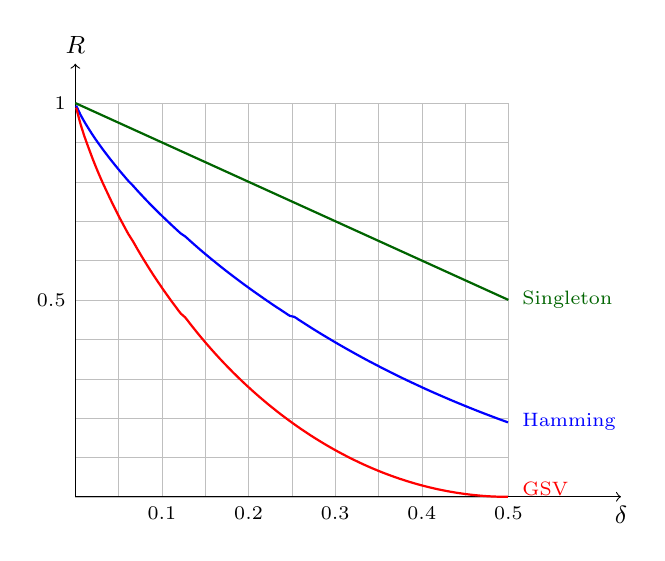
\begin{tikzpicture}[x=11cm,y=5cm]
	\draw[ultra thin,color=lightgray] (0,0) grid[xstep=0.05,ystep=0.1] (0.5,1);
	\draw[->,thin] (0,0) -- (0.63,0) node[below,font=\small] {$\delta$};
	\draw[->,thin] (0,0) -- (0,1.1) node[above,font=\small] {$R$};
	\foreach \x/\l in {0.1/0.1, 0.2/0.2, 0.3/0.3, 0.4/0.4, 0.5/0.5}
		\node[font=\scriptsize,below] at (\x,0) {$\l$};
	\foreach \y/\l in {0.5/0.5, 1/1}
		\node[font=\scriptsize,left] at (0,\y) {$\l$};
	% Hamming bound R = 1 - H(delta/2)
	\draw[thick,color=blue,smooth,samples=100,domain=0.001:0.5]
		plot (\x, {1 + ((\x/2)*ln(\x/2) + (1-\x/2)*ln(1-\x/2))/ln(2)});
	% Singleton bound R = 1 - delta
	\draw[thick,color=DarkGreen] (0,1) -- (0.5,0.5);
	% GSV bound R = 1 - H(delta)
	\draw[thick,color=red,smooth,samples=100,domain=0.001:0.4999]
		plot (\x, {1 + (\x*ln(\x) + (1-\x)*ln(1-\x))/ln(2)});
	\node[font=\scriptsize,color=DarkGreen,anchor=west] at (0.505,0.50) {Singleton};
	\node[font=\scriptsize,color=blue,anchor=west] at (0.505,0.19) {Hamming};
	\node[font=\scriptsize,color=red,anchor=west] at (0.505,0.02) {GSV};
\end{tikzpicture}
\end{center}

Anything achievable lies below the blue and green curves and, by GSV, at least the region below the red curve \emph{is} achievable. The gap between red and blue is enormous, and closing it -- determining the true asymptotic trade-off between rate and distance -- remains one of the central open problems of coding theory.

\subsection{Constructing New Codes from Old}

We finish this section with three easy operations on codes; each is worth knowing because they let us move around the parameter space by hand. Let $C$ be an $[n,m,d]$-code.

\begin{example}[Parity Check Extension]
	The \vocab{parity check extension} of $C$ is
	$$C^+ = \Bigl\{\Bigl(c_1, \dots, c_n, \sum_{i=1}^n c_i\Bigr) : (c_1,\dots,c_n) \in C\Bigr\},$$
	an $[n+1,m,d']$-code where $d' = d+1$ if $d$ is odd and $d' = d$ if $d$ is even. (All codewords of $C^+$ have even weight, so distances between them are even; hence an odd $d$ must increase.)
\end{example}

\begin{example}[Punctured Code]
	Deleting the $i$th digit from every codeword gives the \vocab{punctured code} $C^-$. If $d \ge 2$ this is an $[n-1,m,d']$-code with $d' \in \{d-1, d\}$; the codewords remain distinct because they differed in at least two places.
\end{example}

\begin{example}[Shortened Code]
	Fix $i$ and $\alpha \in \F_2$, and let
	$$C' = \{(c_1,\dots,c_{i-1},c_{i+1},\dots,c_n) : (c_1,\dots,c_{i-1},\alpha,c_{i+1},\dots,c_n) \in C\}.$$
	This is the \vocab{shortened code}. It has length $n-1$ and minimum distance $d' \ge d$, and for a suitable choice of $\alpha$ (namely, the more popular value of the $i$th digit) it has size $m' \ge \frac{m}{2}$.
\end{example}


\section{Information Theory}\label{sec:infotheory}

We now have two loose ends to tie up. In Section~2 we measured the cost of encoding a \emph{single} symbol and found the entropy $H(X)$ standing in the way; but a real source emits a long stream of symbols, possibly with dependence between them, and we should ask what the cost per symbol is in the long run. In Section~3 we defined the capacity of a channel and did not compute it for a single example. Both questions are answered by the same circle of ideas, and the answers are Shannon's two coding theorems.

\subsection{Sources and Information Rate}

\begin{definition}[Source]
	A \vocab{source} is a sequence of random variables $X_1, X_2, \dots$ taking values in an alphabet $\Ac$.
\end{definition}

\begin{example}
	A \vocab{Bernoulli} or \vocab{memoryless} source is one in which the $X_i$ are independent and identically distributed. English text is emphatically not of this kind -- the letter $u$ is much more likely after a $q$ -- but it is the case in which everything can be computed.
\end{example}

\begin{definition}[Reliable Encoding]
	A source $X_1, X_2, \dots$ is \vocab{reliably encodable at rate $r$} if there are subsets $A_n \subseteq \Ac^n$ with
	\begin{enumerate}[label=(\roman*)]
		\item $\displaystyle \lim_{n\to\infty} \frac{\log \abs{A_n}}{n} = r$, and
		\item $\displaystyle \lim_{n\to\infty} \PP\bigl((X_1,\dots,X_n) \in A_n\bigr) = 1$.
	\end{enumerate}
	The \vocab{information rate} $H$ of the source is the infimum of all rates at which it is reliably encodable.
\end{definition}

The idea is that we agree to encode faithfully only the messages in $A_n$, which takes $\log\abs{A_n}$ bits, and accept a vanishing probability of complete failure otherwise. Since $A_n = \Ac^n$ always works, $H \le \log\abs{\Ac}$; and clearly $H \ge 0$. Both extremes occur.

Before going further, a piece of notation which is easy to misread. If $X$ is a discrete random variable with probability mass function $p_X(x) = \PP(X = x)$, then $p(X)$ denotes the composite $p_X \circ X$, that is, the random variable
$$\omega \mapsto \PP\bigl(X = X(\omega)\bigr).$$
It is the `probability of what actually happened'. Similarly, given a tuple of random variables $X^{(n)} = (X_1, \dots, X_n)$, we write $p(X^{(n)})$ for
$$\omega \mapsto \PP\bigl(X_1 = X_1(\omega), \dots, X_n = X_n(\omega)\bigr).$$
With this notation, $H(X) = \EE[-\log p(X)]$.

\begin{example}
	Let $\Ac = \{A,B,C\}$ and suppose that $X^{(2)} = (X_1,X_2)$ takes the six values
	$$AB,\quad AC,\quad BC,\quad BA,\quad CA,\quad CB$$
	with probabilities $0.3$, $0.1$, $0.1$, $0.2$, $0.25$, $0.05$ respectively. Then $p_{X^{(2)}}(AB) = 0.3$ and so on, so the random variable $p(X^{(2)})$ takes the value $0.3$ with probability $0.3$, the value $0.1$ with probability $0.2$ (there are two outcomes of probability $0.1$), the value $0.2$ with probability $0.2$, and so on.
\end{example}

Recall from IA Probability that $X_n \to L$ \vocab{in probability}, written $X_n \xrightarrow{\PP} L$, if $\PP(\abs{X_n - L} > \varepsilon) \to 0$ for every $\varepsilon > 0$, and that the weak law of large numbers says that if $Y_1, Y_2, \dots$ are i.i.d.\ real random variables with finite mean then $\frac1n \sum_{i \le n} Y_i \xrightarrow{\PP} \EE[Y_1]$.

\begin{example}\label{ex:bernoulliaep}
	Let $X_1, X_2, \dots$ be a Bernoulli source. Then $p(X_1), p(X_2), \dots$ are i.i.d., and by independence
	$$p(X_1, \dots, X_n) = p(X_1)p(X_2)\cdots p(X_n).$$
	Applying the weak law to the i.i.d.\ variables $-\log p(X_i)$,
	$$-\frac1n \log p(X_1,\dots,X_n) = -\frac1n \sum_{i=1}^n \log p(X_i) \xrightarrow{\ \PP\ } \EE\bigl[-\log p(X_1)\bigr] = H(X_1).$$
\end{example}

This last observation is the key to everything in this section, and it deserves a name; but first let us see that it gives the right answer for Bernoulli sources by an elementary route.

\begin{lemma}\label{lem:ratebound}
	The information rate of a Bernoulli source $X_1, X_2, \dots$ is at most the expected word length of an optimal binary code $c$ for $X_1$.
\end{lemma}

\begin{proof}
	Let $L_i$ be the length of the codeword $c(X_i)$, so the $L_i$ are i.i.d.\ with mean $\EE[L_1]$. Fix $\varepsilon>0$ and let
	$$A_n = \bigl\{x \in \Ac^n : c^\star(x) \text{ has length} < n(\EE[L_1]+\varepsilon)\bigr\}.$$
	Then
	$$\PP\bigl((X_1,\dots,X_n) \in A_n\bigr) = \PP\Bigl(\tfrac1n\sum_{i=1}^n L_i < \EE[L_1]+\varepsilon\Bigr) \to 1$$
	by the weak law. Since $c$ is decipherable, $c^\star$ is injective, and there are fewer than $2^{n(\EE[L_1]+\varepsilon)+1}$ binary strings of length less than $n(\EE[L_1]+\varepsilon)$; so
	$$\abs{A_n} \le 2^{n(\EE[L_1]+\varepsilon)+1}.$$
	Enlarging $A_n$ if necessary so that $\abs{A_n} = \floor{2^{n(\EE[L_1]+\varepsilon)}}$ (which only helps condition (ii)), we get $\frac1n\log\abs{A_n}\to \EE[L_1]+\varepsilon$. Hence the source is reliably encodable at rate $\EE[L_1]+\varepsilon$ for every $\varepsilon>0$, and the result follows.
\end{proof}

\begin{corollary}\label{cor:ratelt}
	A Bernoulli source has information rate $H < H(X_1)+1$.
\end{corollary}

\begin{proof}
	Combine Lemma~\ref{lem:ratebound} with the upper bound in Shannon's noiseless coding theorem (Theorem~\ref{thm:noiseless}).
\end{proof}

The `$+1$' is the same waste we met before, and the same trick removes it. Suppose we encode in blocks of size $N$: set $Y_1 = (X_1,\dots,X_N)$, $Y_2 = (X_{N+1},\dots,X_{2N})$ and so on, giving a source over the alphabet $\Ac^N$. One checks directly from the definition that if $(X_i)$ has information rate $H$ then $(Y_j)$ has information rate $NH$.

\begin{proposition}\label{prop:rateleH}
	The information rate $H$ of a Bernoulli source satisfies $H \le H(X_1)$.
\end{proposition}

\begin{proof}
	The blocked source $(Y_j)$ is again Bernoulli, so Corollary~\ref{cor:ratelt} applies to it:
	$$NH < H(Y_1) + 1 = H(X_1,\dots,X_N)+1 = NH(X_1)+1,$$
	the last equality by independence and Lemma~\ref{lem:subadd} (with equality since the $X_i$ are independent). Dividing by $N$ gives $H < H(X_1)+\frac1N$ for every $N$.
\end{proof}

\subsection{The Asymptotic Equipartition Property}

Example~\ref{ex:bernoulliaep} isolates exactly the property we need, and it is worth abstracting.

\begin{definition}[AEP]
	A source $X_1, X_2, \dots$ satisfies the \vocab{asymptotic equipartition property} (AEP) with constant $H \ge 0$ if
	$$-\frac1n\log p(X_1,\dots,X_n) \xrightarrow{\ \PP\ } H.$$
\end{definition}

\begin{example}
	Toss a biased coin with $\PP(\text{head}) = q$, and let $X_1, X_2, \dots$ record the results. After $N$ tosses we expect about $qN$ heads, and any \emph{particular} sequence with exactly $qN$ heads has probability
	$$q^{qN}(1-q)^{(1-q)N} = 2^{N(q\log q + (1-q)\log(1-q))} = 2^{-NH(q)}.$$
	Not every sequence looks like this; but the atypical ones carry vanishing total probability. So with high probability we see a `typical sequence', and typical sequences are all roughly \emph{equally likely}, each with probability about $2^{-NH(q)}$. This is what the name is describing: the probability mass is asymptotically spread evenly over about $2^{NH}$ sequences.
\end{example}

That reformulation is worth recording precisely.

\begin{lemma}\label{lem:typical}
	A source satisfies the AEP with constant $H$ if and only if for every $\varepsilon>0$ there is $n_0$ such that for all $n \ge n_0$ there is a \vocab{typical set} $T_n \subseteq \Ac^n$ with
	\begin{enumerate}[label=(\roman*)]
		\item $\PP\bigl((X_1,\dots,X_n) \in T_n\bigr) > 1-\varepsilon$;
		\item $2^{-n(H+\varepsilon)} \le p(x_1,\dots,x_n) \le 2^{-n(H-\varepsilon)}$ for all $(x_1,\dots,x_n) \in T_n$.
	\end{enumerate}
\end{lemma}

\begin{proof}
	Suppose the AEP holds and let $\varepsilon>0$. Define
	$$T_n = \Bigl\{(x_1,\dots,x_n) : \Bigl\lvert-\tfrac1n \log p(x_1,\dots,x_n) - H\Bigr\rvert \le \varepsilon\Bigr\},$$
	which is precisely the set on which (ii) holds. By convergence in probability, $\PP((X_1,\dots,X_n)\in T_n) \to 1$, so (i) holds for $n$ large.

	Conversely, given such sets $T_n$, for any $\varepsilon > 0$ we have
	$$\PP\Bigl(\Bigl\lvert-\tfrac1n\log p(X_1,\dots,X_n)-H\Bigr\rvert \le \varepsilon\Bigr) \ge \PP\bigl((X_1,\dots,X_n)\in T_n\bigr) > 1-\varepsilon$$
	for $n \ge n_0(\varepsilon)$, which is convergence in probability.
\end{proof}

\subsection{Shannon's First Coding Theorem}

\begin{theorem}[Shannon's First Coding Theorem]\label{thm:firstcoding}
	A source satisfying the AEP with constant $H$ has information rate exactly $H$.
\end{theorem}

\begin{proof}
	\emph{Rate $H$ is achievable.} Let $\varepsilon>0$ and take typical sets $T_n$ as in Lemma~\ref{lem:typical}. For $n \ge n_0(\varepsilon)$ and $(x_1,\dots,x_n) \in T_n$ we have $p(x_1,\dots,x_n) \ge 2^{-n(H+\varepsilon)}$, so
	$$1 \ge \PP(T_n) \ge \abs{T_n}\,2^{-n(H+\varepsilon)}, \qquad \text{giving} \qquad \frac1n \log\abs{T_n} \le H+\varepsilon.$$
	Taking $A_n = T_n$ (padded if necessary so that the limit in (i) exists and equals $H + \varepsilon$) shows that the source is reliably encodable at rate $H+\varepsilon$. As $\varepsilon>0$ was arbitrary, the information rate is at most $H$.

	\emph{No smaller rate is achievable.} If $H=0$ there is nothing to prove, so assume $H>0$ and let $0 < \varepsilon < \tfrac{H}{2}$. Suppose for contradiction that the source is reliably encodable at rate $H-2\varepsilon$, witnessed by sets $A_n$. Let $T_n$ be typical sets for this $\varepsilon$. For $(x_1,\dots,x_n)\in T_n$ we have $p(x_1,\dots,x_n) \le 2^{-n(H-\varepsilon)}$, so
	$$\PP\bigl((X_1,\dots,X_n) \in A_n \cap T_n\bigr) \le \abs{A_n}\,2^{-n(H-\varepsilon)},$$
	and hence
	$$\frac1n\log \PP(A_n \cap T_n) \le -(H-\varepsilon) + \frac1n\log\abs{A_n} \longrightarrow -(H-\varepsilon)+(H-2\varepsilon) = -\varepsilon.$$
	Therefore $\log\PP(A_n \cap T_n) \to -\infty$, so $\PP(A_n \cap T_n) \to 0$. But
	$$\PP(T_n) \le \PP(A_n \cap T_n) + \PP(\Ac^n \setminus A_n) \to 0 + 0 = 0,$$
	contradicting $\PP(T_n) > 1-\varepsilon$. So the information rate is at least $H$.
\end{proof}

\begin{corollary}
	A Bernoulli source has information rate exactly $H(X_1)$.
\end{corollary}

\begin{proof}
	Example~\ref{ex:bernoulliaep} verifies the AEP with constant $H(X_1)$.
\end{proof}

\begin{remark}
	The theorem is not merely an existence statement; it comes with a coding scheme. Encode the typical sequences with a block code of length $\ceil{n(H+\varepsilon)}$, and encode the atypical sequences however you like (say, by a reserved escape symbol followed by the raw string). The scheme fails with vanishing probability and costs $H+\varepsilon$ bits per symbol.

	Many non-Bernoulli sources also satisfy the AEP. Under suitable hypotheses -- for instance for a stationary ergodic source -- the sequence $\frac1n H(X_1,\dots,X_n)$ is decreasing, and the AEP holds with $H = \lim_n \frac1n H(X_1,\dots,X_n)$. This is what makes the theory applicable to real text.
\end{remark}

\subsection{Capacity of the Binary Symmetric Channel}

We now turn to the channel side. Recall the definitions from Section~1: a code of length $n$ is $C \subseteq \Ac^n$, its rate is $\rho(C) = \frac{\log\abs{C}}{n}$, its error rate is $\hat e(C) = \max_{c \in C}\PP(\text{error}\mid c \text{ sent})$, and the capacity is the supremum of rates at which reliable transmission is possible.

As a warm-up -- and because it shows exactly where the GSV bound earns its keep -- let us prove directly that a reasonably good binary symmetric channel has positive capacity.

\begin{lemma}\label{lem:wlln}
	Let $\varepsilon>0$ and let a BSC with error probability $p$ be used $n$ times. Then
	$$\lim_{n\to\infty}\PP\bigl(\text{the channel makes at least } n(p+\varepsilon) \text{ errors}\bigr) = 0.$$
\end{lemma}

\begin{proof}
	Let $U_i$ be the indicator that the $i$th digit is mistransmitted. The $U_i$ are i.i.d.\ with $\EE[U_i] = p$, and
	$$\PP\Bigl(\sum_{i=1}^n U_i \ge n(p+\varepsilon)\Bigr) \le \PP\Bigl(\Bigl\lvert\tfrac1n\sum_{i=1}^n U_i - p\Bigr\rvert \ge \varepsilon\Bigr) \to 0$$
	by the weak law of large numbers.
\end{proof}

\begin{proposition}
	A binary symmetric channel with error probability $p < \tfrac14$ has nonzero capacity.
\end{proposition}

\begin{proof}
	Choose $\delta$ with $2p < \delta < \tfrac12$; this is possible precisely because $p< \tfrac14$. We claim we can transmit reliably at rate $R = 1-H(\delta) > 0$.

	Let $C_n$ be an $[n, A(n,\floor{n\delta}), \floor{n\delta}]$-code of maximal size. By the GSV bound and Proposition~\ref{prop:volbound},
	$$\abs{C_n} = A(n,\floor{n\delta}) \ge 2^{n(1-H(\delta))} = 2^{nR},$$
	and passing to a subcode we may assume $\abs{C_n} = \floor{2^{nR}}$, still with minimum distance at least $\floor{n\delta}$. Using minimum distance decoding, an error occurs only if the channel makes more than $\floor{\frac{\floor{n\delta}-1}{2}}$ errors, so
	$$\hat e(C_n) \le \PP\Bigl(\text{at least } \tfrac{n\delta-1}{2} \text{ errors in } n \text{ uses}\Bigr).$$
	Now pick $\varepsilon>0$ with $p+\varepsilon < \frac{\delta}{2}$, which is possible as $2p<\delta$. For large $n$,
	$$\frac{n\delta-1}{2} = n\Bigl(\frac{\delta}{2}-\frac{1}{2n}\Bigr) > n(p+\varepsilon),$$
	so $\hat e(C_n) \le \PP(\text{at least } n(p+\varepsilon) \text{ errors})\to 0$ by Lemma~\ref{lem:wlln}. Since $\rho(C_n)\to R$, we are done.
\end{proof}

This is already remarkable, but the constant is wrong: the answer is not $1-H(\delta)$ for some $\delta > 2p$, and the restriction $p< \tfrac14$ is an artefact. To get the truth we need a more delicate measure of how much a channel destroys.

\subsection{Conditional Entropy and Fano's Inequality}

\begin{definition}[Conditional Entropy]
	Let $X, Y$ take values in $\Ac, \Bc$. The \vocab{conditional entropy} of $X$ given $Y = y$ is
	$$H(X \mid Y=y) = -\sum_{x \in \Ac}\PP(X = x\mid Y=y)\log\PP(X=x\mid Y=y),$$
	and the \vocab{conditional entropy} of $X$ given $Y$ is
	$$H(X\mid Y) = \sum_{y\in\Bc}\PP(Y=y)\,H(X\mid Y=y).$$
\end{definition}

Clearly $H(X\mid Y)\ge0$. It measures how much uncertainty about $X$ remains once $Y$ is known.

\begin{lemma}[Chain Rule]\label{lem:chain}
	$H(X,Y) = H(X\mid Y) + H(Y)$.
\end{lemma}

\begin{proof}
	Expanding the definition and writing $\PP(X = x \mid Y = y)\PP(Y=y) = \PP(X=x,Y=y)$,
	\begin{align*}
		H(X\mid Y) &= -\sum_{y}\sum_x \PP(X=x,Y=y)\log\frac{\PP(X=x,Y=y)}{\PP(Y=y)}\\
		&= -\sum_{y}\sum_x \PP(X=x,Y=y)\log\PP(X=x,Y=y)\\
		&\qquad + \sum_y \Bigl(\sum_x\PP(X=x,Y=y)\Bigr)\log\PP(Y=y)\\
		&= H(X,Y) + \sum_y \PP(Y=y)\log\PP(Y=y) = H(X,Y)-H(Y). \qedhere
	\end{align*}
\end{proof}

\begin{example}
	Let $X$ be uniform on $\{1,\dots,6\}$, modelling a die, and let $Y$ be $0$ if $X$ is even and $1$ if $X$ is odd. Then $Y$ is a function of $X$, so $H(X,Y)=H(X)=\log 6$, and $H(Y)=\log2 = 1$. The chain rule gives $H(X\mid Y) = \log 6 - \log 2 = \log 3$, which is right: knowing the parity leaves three equally likely values. Applying the chain rule the other way round, $H(Y\mid X) = H(X,Y)-H(X) = 0$, as it must be.
\end{example}

\begin{corollary}\label{cor:condle}
	$H(X\mid Y)\le H(X)$, with equality if and only if $X$ and $Y$ are independent.
\end{corollary}

\begin{proof}
	Combine the chain rule with subadditivity (Lemma~\ref{lem:subadd}): $H(X\mid Y) = H(X,Y)-H(Y) \le H(X)$, with the same equality condition.
\end{proof}

Everything extends to tuples: replacing $X$ by $X^{(r)} = (X_1,\dots,X_r)$ and $Y$ by $Y^{(s)}$, we may speak of $H(X_1,\dots,X_r\mid Y_1,\dots,Y_s)$. One must read such expressions carefully: $H(X,Y\mid Z)$ is the entropy of the \emph{pair} $(X,Y)$ given $Z$, not the entropy of $X$ together with the entropy of $Y$ given $Z$.

\begin{lemma}\label{lem:threevar}
	$H(X\mid Y) \le H(X\mid Y,Z) + H(Z)$.
\end{lemma}

\begin{proof}
	Expand $H(X,Y,Z)$ in two ways using the chain rule:
	$$H(Z\mid X,Y) + \underbrace{H(X\mid Y)+H(Y)}_{H(X,Y)} = H(X,Y,Z) = H(X\mid Y,Z)+\underbrace{H(Z\mid Y)+H(Y)}_{H(Y,Z)}.$$
	Since $H(Z\mid X,Y)\ge0$ we get $H(X\mid Y) \le H(X\mid Y,Z)+H(Z\mid Y)$, and $H(Z\mid Y)\le H(Z)$ by Corollary~\ref{cor:condle}.
\end{proof}

Now for the key estimate. Think of $X$ as what was sent and $Y$ as what was decoded; then $p = \PP(X\ne Y)$ is the probability of error, and Fano's inequality bounds how much uncertainty can remain.

\begin{proposition}[Fano's Inequality]\label{prop:fano}
	Let $X,Y$ take values in an alphabet $\Ac$ with $\abs{\Ac} = m \ge 2$, and let $p = \PP(X\ne Y)$. Then
	$$H(X\mid Y) \le H(p) + p\log(m-1).$$
\end{proposition}

\begin{proof}
	Let $Z$ be the indicator of the event $X \ne Y$, so $H(Z) = H(p)$. By Lemma~\ref{lem:threevar} it suffices to show $H(X\mid Y,Z)\le p\log(m-1)$.

	If $Z = 0$ then $X = Y$, so $H(X\mid Y=y,Z=0) = 0$. If $Z=1$ then $X$ is one of the $m-1$ values other than $y$, so $H(X\mid Y=y,Z=1)\le\log(m-1)$. Hence
	\begin{align*}
		H(X\mid Y,Z) &= \sum_{y\in\Ac}\sum_{z\in\{0,1\}}\PP(Y=y,Z=z)\,H(X\mid Y=y,Z=z)\\
		&\le \sum_{y\in\Ac}\PP(Y=y,Z=1)\log(m-1)\\
		&= \PP(Z=1)\log(m-1) = p\log(m-1). \qedhere
	\end{align*}
\end{proof}

The two terms have a clean reading: $H(p)$ is the information needed to say \emph{whether} an error occurred, and $p\log(m-1)$ is the information needed to say \emph{which} error it was, in the worst case.

\subsection{Mutual Information and Information Capacity}

\begin{definition}[Mutual Information]
	The \vocab{mutual information} of $X$ and $Y$ is
	$$I(X;Y) = H(X)-H(X\mid Y).$$
\end{definition}

By the chain rule $I(X;Y) = H(X)+H(Y)-H(X,Y)$, from which it is visibly symmetric in $X$ and $Y$, and non-negative by subadditivity, with $I(X;Y)=0$ if and only if $X$ and $Y$ are independent. It measures how much knowing one variable tells us about the other -- exactly the quantity a channel ought to be judged by.

\begin{definition}[Information Capacity]
	Let a discrete memoryless channel have input alphabet $\Ac$ and output alphabet $\Bc$. For a random variable $X$ on $\Ac$, let $Y$ be the resulting output. The \vocab{information capacity} of the channel is
	$$C = \max_X I(X;Y),$$
	the maximum being over all distributions of $X$ on $\Ac$.
\end{definition}

This maximum really is attained, since $I$ is a continuous function of the input distribution $(p_1,\dots,p_m)$, which ranges over the compact simplex $\{p_i \ge 0, \sum p_i = 1\}$. Note that the information capacity depends only on the channel matrix, and is a finite computation; whereas the (operational) capacity of Section~1 is defined by a limiting process over all possible codes. The content of Shannon's second theorem is that they agree.

\begin{theorem}[Shannon's Noisy Coding Theorem]\label{thm:secondcoding}
	For a discrete memoryless channel, the operational capacity equals the information capacity.
\end{theorem}

We shall prove the inequality `operational $\le$ information' in general, and the reverse inequality for the binary symmetric channel. First, let us see what the theorem buys us.

\begin{example}\label{ex:capacities}
	\begin{enumerate}[label=(\roman*)]
		\item \emph{The binary symmetric channel with error probability $p$.} Let $\PP(X=0)=\alpha$. Given $X$, the output differs from the input with probability $p$ regardless, so $H(Y\mid X=0)=H(Y\mid X=1)=H(p)$ and hence $H(Y\mid X) = H(p)$. Also $\PP(Y=0) = \alpha(1-p)+(1-\alpha)p$. Therefore
		\begin{align*}
			C &= \max_\alpha\bigl[H(Y)-H(Y\mid X)\bigr]\\
			&= \max_\alpha \bigl[H\bigl(\alpha(1-p)+(1-\alpha)p\bigr)-H(p)\bigr] = 1-H(p),
		\end{align*}
		the maximum being at $\alpha = \tfrac12$, when the argument of the outer $H$ is $\tfrac12$. So
		$$C = 1 + p\log p + (1-p)\log(1-p).$$
		If $p = 0$ or $p=1$ then $C=1$; if $p = \tfrac12$ then $C = 0$, confirming that such a channel is useless.
		\item \emph{The binary erasure channel with erasure probability $p$.} Here it is easier to compute $I(Y;X) = H(X)-H(X\mid Y)$. With $\PP(X=0)=\alpha$, receiving $0$ or $1$ determines $X$, so $H(X\mid Y=0)=H(X\mid Y=1)=0$, while $H(X\mid Y=\star) = H(\alpha)$. As $\PP(Y=\star)=p$,
		$$C = \max_\alpha\bigl[H(\alpha)-pH(\alpha)\bigr] = (1-p)\max_\alpha H(\alpha) = 1-p,$$
		again at $\alpha=\tfrac12$. This is exactly what one would guess: a fraction $p$ of the transmissions is simply lost.
	\end{enumerate}
\end{example}

Note the strength of the first computation. A channel that flips one bit in ten has capacity $1-H(0.1) = 0.531$, so we can push more than half a bit of genuine information through each use of it, with arbitrarily small error probability.

\begin{lemma}\label{lem:extcap}
	If a discrete memoryless channel has information capacity $C$, its $n$th extension has information capacity $nC$.
\end{lemma}

\begin{proof}
	Let $X_1,\dots,X_n$ be the input and $Y_1,\dots,Y_n$ the output. Because the channel is memoryless, $Y_i$ depends only on $X_i$, so
	$$H(Y_1,\dots,Y_n\mid X_1,\dots,X_n) = \sum_{i=1}^n H(Y_i\mid X_1,\dots,X_n) = \sum_{i=1}^n H(Y_i\mid X_i).$$
	Hence, using subadditivity for the first term,
	\begin{align*}
		I(X_1,\dots,X_n;Y_1,\dots,Y_n) &= H(Y_1,\dots,Y_n)-H(Y_1,\dots,Y_n\mid X_1,\dots,X_n)\\
		&\le \sum_{i=1}^n H(Y_i)-\sum_{i=1}^n H(Y_i\mid X_i) = \sum_{i=1}^n I(X_i;Y_i) \le nC.
	\end{align*}
	Conversely, take the $X_i$ independent and each achieving $I(X_i;Y_i)=C$. Then the $Y_i$ are independent too, so $H(Y_1,\dots,Y_n) = \sum_i H(Y_i)$ and the first inequality is an equality. Hence the maximum is exactly $nC$.
\end{proof}

\subsection{Proof of the Noisy Coding Theorem}\label{sec:noisycoding}

We begin with the converse, which holds for any discrete memoryless channel.

\begin{proposition}[Converse to the Noisy Coding Theorem]
	The operational capacity of a discrete memoryless channel is at most its information capacity $C$.
\end{proposition}

\begin{proof}
	Suppose, for contradiction, that reliable transmission is possible at some rate $R > C$. Then there are codes $C_n$ of length $n$ and size $\floor{2^{nR}}$ with $\rho(C_n)\to R$ and $\hat e(C_n)\to0$.

	Introduce the \vocab{average error rate}
	$$e(C_n) = \frac{1}{\abs{C_n}}\sum_{c\in C_n}\PP(\text{error}\mid c\text{ sent}) \le \hat e(C_n),$$
	so $e(C_n)\to0$ as well. Let $X$ be uniform on $C_n$, let $Y$ be the channel output, and let $\hat X$ be the decoded codeword; write $p = e(C_n) = \PP(X \ne \hat X)$.

	Since $X$ is uniform, $H(X) = \log\abs{C_n} = \log\floor{2^{nR}} \ge nR-1$ for $n$ large. By Fano's inequality applied to $X$ and $\hat X$, and then the fact that $\hat X$ is a function of $Y$ (so conditioning on $Y$ can only be more informative),
	$$H(X\mid Y) \le H(X \mid \hat X) \le H(p)+p\log(\abs{C_n}-1) \le 1 + pnR.$$
	Therefore, using Lemma~\ref{lem:extcap} for the $n$th extension,
	$$nC \ge I(X;Y) = H(X)-H(X\mid Y) \ge (nR-1)-(1+pnR),$$
	so that
	$$p\,nR \ge n(R-C)-2, \qquad\text{that is}\qquad p \ge \frac{n(R-C)-2}{nR} \longrightarrow \frac{R-C}{R} > 0.$$
	This contradicts $p = e(C_n)\to0$. Hence no rate above $C$ is achievable.
\end{proof}

The direct half is the celebrated one, and Shannon's proof is a masterpiece of the probabilistic method: rather than constructing a good code, we pick one at random and show that the average is good enough.

\begin{proposition}\label{prop:randomcoding}
	Let a BSC have error probability $p$, and let $R < 1-H(p)$. Then there are codes $C_n$ of length $n$ and size $\floor{2^{nR}}$ with $\rho(C_n)\to R$ and $e(C_n)\to0$.
\end{proposition}

Note that this concerns the \emph{average} error rate $e$; we shall upgrade to $\hat e$ afterwards.

\begin{proof}
	Without loss of generality $p< \tfrac12$. Choose $\varepsilon>0$ small enough that $p+\varepsilon<\tfrac12$ and $R < 1-H(p+\varepsilon)$; this is possible by continuity of $H$. Put $m = \floor{2^{nR}}$ and $r = \floor{n(p+\varepsilon)}$. We use minimum distance decoding, breaking ties arbitrarily.

	Let $\Cc$ be the set of all $[n,m]$-codes, so $\abs{\Cc} = \binom{2^n}{m}$, and choose $C = \{c_1,\dots,c_m\}$ from $\Cc$ uniformly at random. Choose $i \in \{1,\dots,m\}$ uniformly at random too, send $c_i$, and let $Y$ be the output. Then
	$$\PP(Y \text{ not decoded as } c_i) = \frac{1}{\abs{\Cc}}\sum_{C \in \Cc} e(C),$$
	so there exists some $C_n \in \Cc$ with $e(C_n)$ at most this average. It therefore suffices to show that the left hand side tends to $0$.

	If $B(Y,r)\cap C = \{c_i\}$ then $Y$ is certainly decoded as $c_i$, so
	$$\PP(Y\text{ not decoded as }c_i) \le \PP\bigl(c_i \notin B(Y,r)\bigr) + \PP\bigl(B(Y,r)\cap C \supsetneq \{c_i\}\bigr),$$
	and we handle the two terms separately.

	The first term is $\PP(d(c_i,Y)>r)$, which is the probability that the channel makes more than $n(p+\varepsilon)$ errors; this tends to $0$ by Lemma~\ref{lem:wlln}.

	For the second term, condition on $Y$ and on $c_i$. Given that $c_i \in B(Y,r)$, each of the other $m-1$ codewords is uniform over the remaining $2^n - 1$ words, so
	$$\PP\bigl(c_j \in B(Y,r)\mid c_i \in B(Y,r)\bigr) = \frac{V(n,r)-1}{2^n-1}\le \frac{V(n,r)}{2^n}$$
	for $j \ne i$. Hence, by a union bound and Proposition~\ref{prop:volbound}(i),
	\begin{align*}
		\PP\bigl(B(Y,r)\cap C \supsetneq \{c_i\}\bigr) &\le \sum_{j\ne i}\PP\bigl(c_j\in B(Y,r)\mid c_i \in B(Y,r)\bigr)\\
		&\le (m-1)\frac{V(n,r)}{2^n} \le 2^{nR}\,2^{nH(p+\varepsilon)}\,2^{-n}\\
		&= 2^{-n\left(1-H(p+\varepsilon)-R\right)} \longrightarrow 0,
	\end{align*}
	because $R < 1-H(p+\varepsilon)$. This completes the proof.
\end{proof}

\begin{proposition}
	In Proposition~\ref{prop:randomcoding} we may replace $e$ by $\hat e$.
\end{proposition}

\begin{proof}
	Choose $R'$ with $R<R'<1-H(p)$ and apply the previous proposition to $R'$, obtaining codes $C_n'$ of size $\floor{2^{nR'}}$ with $e(C_n')\to0$. Order the codewords of $C_n'$ by their individual error probabilities and delete the worse half, giving a code $C_n''$. If more than half the codewords had error probability exceeding $2e(C_n')$ the average would exceed $e(C_n')$; so $\hat e(C_n'')\le 2e(C_n')\to0$. Now $C_n''$ has size $\tfrac12\floor{2^{nR'}} \ge 2^{nR}$ for large $n$, since $2^{nR'-1} = 2^{n(R'-1/n)} \ge 2^{nR}$ eventually. Passing to a subcode of size exactly $\floor{2^{nR}}$ can only decrease $\hat e$, and gives $\rho \to R$.
\end{proof}

Putting the two halves together: the binary symmetric channel with error probability $p$ has operational capacity exactly $1 - H(p)$, which by Example~\ref{ex:capacities} is also its information capacity. This is Theorem~\ref{thm:secondcoding} for the BSC.

\begin{remark}
	The proof is purely existential. It tells us that almost every code of the right size is good, but it gives no way of writing one down, and no way of decoding one efficiently even if we could -- minimum distance decoding over $2^{nR}$ codewords is hopeless. Finding explicit families of codes approaching capacity, with practical decoding algorithms, took another fifty years. The rest of these notes on coding theory is about algebraic constructions which are far from optimal but eminently practical.
\end{remark}

\subsection{An Aside: the Kelly Criterion}

Entropy turns up in places that have nothing obviously to do with communication. Here is one, included because it is charming and because it was lectured.

Suppose a biased coin with $\PP(\text{head}) = p$ is tossed repeatedly, and that before each toss we may stake money on heads at odds $u$: a stake of $k$ returns $ku$ if the coin comes up heads and nothing otherwise. Start with a bankroll $X_0 = 1$ and bet a fixed fraction $w \in [0,1)$ of the current bankroll each time, so
$$X_{n+1} = \begin{cases} X_n\bigl(wu + (1-w)\bigr) & \text{if toss } n+1 \text{ is a head},\\ X_n(1-w) & \text{otherwise.}\end{cases}$$
Then $Y_{n+1} = X_{n+1}/X_n$ are i.i.d., and $\log X_n = \sum_{i=1}^n \log Y_i$ is a sum of i.i.d.\ terms.

\begin{lemma}
	Let $\mu = \EE[\log Y_1]$ and $\sigma^2 = \var(\log Y_1)$. Then for $a>0$,
	$$\PP\left(\left\lvert \frac{\log X_n}{n}-\mu\right\rvert \ge a\right) = \PP\left(\left\lvert\frac1n\sum_{i=1}^n \log Y_i - \mu\right\rvert\ge a\right) \le \frac{\sigma^2}{na^2}.$$
	In particular, for any $\varepsilon, \delta>0$ there is $N$ with $\PP(\abs{\frac{\log X_n}{n}-\mu}\ge\delta)\le\varepsilon$ for all $n\ge N$.
\end{lemma}

\begin{proof}
	Immediate from Chebyshev's inequality applied to the sample mean.
\end{proof}

So the bankroll behaves like $2^{n\mu}$, and to do well in the long run we should maximise $\mu$ rather than the expected return. Now
$$\mu = \EE[\log Y] = p\log\bigl(1+(u-1)w\bigr)+(1-p)\log(1-w).$$
Differentiating with respect to $w$ and setting the result to zero, one finds that $\mu$ is maximised at $w = 0$ if $up \le 1$ (the bet is not worth taking) and at
$$w = \frac{up-1}{u-1}$$
if $up>1$. This is \vocab{Kelly's criterion}. Writing $q = 1-p$ and substituting the optimal $w$,
$$\EE[\log Y] = p\log p + q \log q + \log u - q\log(u-1) = -H(p)+\log u - q\log(u-1).$$
Entropy has appeared, and it is exactly the penalty paid for the randomness of the coin. Betting below the Kelly fraction still grows the bankroll, but more slowly; betting sufficiently far above it makes the bankroll tend to zero almost surely, however favourable the odds.


\section{Linear Codes}\label{sec:linear}

Shannon's theorem guarantees good codes but produces none, and even if it did we could not use them, because minimum distance decoding over an unstructured code of size $2^{nR}$ is computationally hopeless. The way out is to insist that our codes be \emph{linear subspaces}, at which point all the machinery of IB Linear Algebra becomes available and both encoding and decoding become matrix arithmetic.

\subsection{Linear Codes, Generator and Parity Check Matrices}

\begin{definition}[Linear Code]
	A binary code $C \subseteq \F_2^n$ is \vocab{linear} if $0 \in C$ and $x+y \in C$ whenever $x,y \in C$; equivalently, if $C$ is a vector subspace of $\F_2^n$.
\end{definition}

\begin{definition}[Rank]
	The \vocab{rank} of a linear code $C$ is its dimension as an $\F_2$-vector space. A linear code of length $n$ and rank $k$ is an \vocab{$(n,k)$-code}; if its minimum distance is $d$ it is an \vocab{$(n,k,d)$-code}.
\end{definition}

We use round brackets for linear codes and square brackets for general ones. If $v_1,\dots,v_k$ is a basis then every codeword is uniquely $\sum \lambda_i v_i$ with $\lambda_i \in \F_2$, so $\abs{C} = 2^k$. Thus an $(n,k)$-code is an $[n,2^k]$-code, and its information rate is $\frac kn$ -- a pleasantly simple formula.

\begin{definition}[Weight]
	The \vocab{weight} of $x \in \F_2^n$ is $\wt(x) = d(x,0)$, the number of nonzero digits.
\end{definition}

\begin{lemma}\label{lem:wtmin}
	The minimum distance of a linear code equals the minimum weight of a nonzero codeword.
\end{lemma}

\begin{proof}
	For $x,y \in \F_2^n$ we have $d(x,y) = d(x+y,0) = \wt(x+y)$, since over $\F_2$ subtraction is addition. If $C$ is linear and $x,y \in C$ are distinct then $x+y$ is a nonzero codeword, and conversely every nonzero codeword $z$ arises as $z = z + 0$. So the two minima are over the same set of numbers.
\end{proof}

This is already a large saving: computing $d(C)$ naively requires $\binom{2^k}{2}$ comparisons, but for a linear code only $2^k - 1$ weights.

\begin{definition}[Dot Product, Dual Code]
	For $x,y \in \F_2^n$ set $x\cdot y = \sum_{i=1}^n x_iy_i \in \F_2$; this is symmetric and bilinear. Given $P \subseteq \F_2^n$, the \vocab{parity check code} defined by $P$ is
	$$C = \{x \in \F_2^n : p\cdot x = 0 \text{ for all } p \in P\}.$$
	For a linear code $C$, the \vocab{dual code} is
	$$C^\perp = \{x \in \F_2^n : x\cdot y = 0 \text{ for all } y \in C\}.$$
\end{definition}

A warning: this bilinear form is not an inner product, since $x\cdot x = 0$ for any $x$ of even weight. In particular $C \cap C^\perp$ need not be $\{0\}$, and a code can even be \emph{self-dual}.

\begin{example}
	\begin{enumerate}[label=(\roman*)]
		\item $P = \{11\dots1\}$ gives the simple parity check code.
		\item $P = \{1010101, 0110011, 0001111\}$ gives Hamming's original $[7,16,3]$-code of Example~\ref{ex:ham74}.
		\item If $C$ is linear then so are the parity check extension $C^+$ and any punctured code $C^-$.
	\end{enumerate}
\end{example}

\begin{lemma}
	Every parity check code is linear.
\end{lemma}

\begin{proof}
	$p\cdot 0 = 0$, and if $p\cdot x = p\cdot y = 0$ then $p\cdot(x+y) = 0$ by bilinearity.
\end{proof}

In particular $C^\perp$ is always linear. We shall shortly see the converse: every linear code is a parity check code.

\begin{definition}[Generator and Parity Check Matrices]
	Let $C$ be an $(n,k)$-code. A \vocab{generator matrix} for $C$ is a $k\times n$ matrix $G$ whose rows form a basis of $C$. A \vocab{parity check matrix} for $C$ is a generator matrix $H$ for $C^\perp$; we shall see it is an $(n-k)\times n$ matrix.
\end{definition}

The two matrices give two descriptions of the same code: codewords are the linear combinations of rows of $G$, and also the linear dependence relations among the columns of $H$,
$$C = \{x \in \F_2^n : Hx = 0\},$$
where we regard $x$ as a column vector. Encoding uses $G$ and decoding uses $H$.

\begin{definition}[Syndrome]
	Let $C$ be a linear code with parity check matrix $H$. The \vocab{syndrome} of $x \in \F_2^n$ is $Hx \in \F_2^{n-k}$.
\end{definition}

Here is the point. Suppose we receive $x = c + z$ where $c \in C$ and $z$ is the error pattern. Since $Hc = 0$,
$$Hx = Hz,$$
so the syndrome depends only on the error, not on the codeword that was sent. If $C$ is $e$-error correcting we may precompute $Hz$ for every $z$ with $\wt(z)\le e$ -- there are $V(n,e)$ of them, far fewer than $2^k$ codewords in general -- and store the results in a table. On receiving $x$ we compute $Hx$, look it up, and decode as $c = x - z$. The cost of decoding is one matrix multiplication and one table lookup.

More generally, two words have the same syndrome exactly when they differ by a codeword, so the syndromes are in bijection with the cosets of $C$ in $\F_2^n$. Minimum distance decoding amounts to choosing, in each coset, a word of least weight -- a \vocab{coset leader} -- and subtracting it. Displaying the cosets as the rows of an array gives the classical picture.

\begin{center}
\begin{tikzpicture}[x=1cm,y=1cm]
	\draw[thin] (-0.2,0.55) -- (7.9,0.55);
	\draw[thin] (0.95,1.05) -- (0.95,-4.1);
	\draw[thin] (6.55,1.05) -- (6.55,-4.1);
	\node[font=\small] at (0.35,0.85)  {$z$};
	\node[font=\small] at (3.7,0.85)   {coset $z + C$};
	\node[font=\small] at (7.25,0.85)  {$Hz$};
	\node[font=\small] at (0.35,0)  {$0$};
	\node[font=\small] at (1.8,0)   {$0$};
	\node[font=\small] at (3.0,0)   {$c_2$};
	\node[font=\small] at (4.2,0)   {$\cdots$};
	\node[font=\small] at (5.6,0)   {$c_m$};
	\node[font=\small] at (7.25,0)  {$0$};
	\node[font=\small] at (0.35,-0.9)  {$z_2$};
	\node[font=\small] at (1.8,-0.9)   {$z_2$};
	\node[font=\small] at (3.0,-0.9)   {$z_2+c_2$};
	\node[font=\small] at (4.2,-0.9)   {$\cdots$};
	\node[font=\small] at (5.6,-0.9)   {$z_2+c_m$};
	\node[font=\small] at (7.25,-0.9)  {$s_2$};
	\node[font=\small] at (0.35,-1.8)  {$z_3$};
	\node[font=\small] at (1.8,-1.8)   {$z_3$};
	\node[font=\small] at (3.0,-1.8)   {$z_3+c_2$};
	\node[font=\small] at (4.2,-1.8)   {$\cdots$};
	\node[font=\small] at (5.6,-1.8)   {$z_3+c_m$};
	\node[font=\small] at (7.25,-1.8)  {$s_3$};
	\node[font=\small] at (0.35,-2.6)  {$\vdots$};
	\node[font=\small] at (1.8,-2.6)   {$\vdots$};
	\node[font=\small] at (3.0,-2.6)   {$\vdots$};
	\node[font=\small] at (5.6,-2.6)   {$\vdots$};
	\node[font=\small] at (7.25,-2.6)  {$\vdots$};
	\node[font=\small] at (0.35,-3.6)  {$z_t$};
	\node[font=\small] at (1.8,-3.6)   {$z_t$};
	\node[font=\small] at (3.0,-3.6)   {$z_t+c_2$};
	\node[font=\small] at (4.2,-3.6)   {$\cdots$};
	\node[font=\small] at (5.6,-3.6)   {$z_t+c_m$};
	\node[font=\small] at (7.25,-3.6)  {$s_t$};
\end{tikzpicture}
\end{center}

The first row is the code itself; the leftmost column holds the coset leaders; the rightmost column holds the syndromes, and it is the only column we need to store. On receiving $x$ we find the row with syndrome $Hx$ and subtract its leader.

\begin{definition}[Equivalence]
	Codes $C_1, C_2 \subseteq \F_2^n$ are \vocab{equivalent} if some permutation of the $n$ coordinates carries $C_1$ onto $C_2$.
\end{definition}

Equivalent codes have the same length, size and minimum distance, so we generally work up to equivalence.

\begin{lemma}\label{lem:standardform}
	Every $(n,k)$-code is equivalent to one with generator matrix in the \vocab{standard form}
	$$G = \begin{pmatrix} I_k & B\end{pmatrix}$$
	for some $k\times(n-k)$ matrix $B$.
\end{lemma}

\begin{proof}
	Let $G$ be any generator matrix. Row operations do not change the row space, so by Gaussian elimination we may put $G$ in row echelon form, with leading $1$s in columns $\ell(1)<\ell(2)<\dots<\ell(k)$. Permuting columns replaces $C$ by an equivalent code, so we may assume $\ell(i)=i$. Further row operations clear the entries above the leading $1$s, leaving $G = (I_k \mid B)$.
\end{proof}

With $G$ in standard form, a message $y \in \F_2^k$ (a row vector) is encoded as
$$yG = (y \mid yB),$$
that is, the message itself followed by $n-k$ \vocab{check digits}. Such an encoding is called \vocab{systematic}, and is convenient because the message can be read straight off the codeword.

\begin{lemma}\label{lem:dualdim}
	For a linear code $C \le \F_2^n$, $\rank C + \rank C^\perp = n$.
\end{lemma}

\begin{proof}
	This is the annihilator statement from IB Linear Algebra, but here is a direct argument. Passing to an equivalent code we may assume $C$ has generator matrix $G = (I_k \mid B)$. Consider the linear map $\gamma\colon \F_2^n \to \F_2^k$, $x \mapsto Gx$. Since $G$ contains $I_k$, its rows are linearly independent, so $\gamma$ is surjective. Its kernel is exactly the set of $x$ orthogonal to every row of $G$, that is, $C^\perp$. By rank--nullity,
	$$n = \dim\ker\gamma + \dim\image\gamma = \rank C^\perp + k. \qedhere$$
\end{proof}

\begin{corollary}
	$(C^\perp)^\perp = C$. In particular every linear code is a parity check code, namely the one defined by $C^\perp$.
\end{corollary}

\begin{proof}
	If $x \in C$ then $x\cdot y = 0$ for all $y \in C^\perp$ by definition, so $C \subseteq (C^\perp)^\perp$. Applying Lemma~\ref{lem:dualdim} twice,
	$$\rank (C^\perp)^\perp = n - \rank C^\perp = n - (n - \rank C) = \rank C,$$
	so the inclusion is an equality.
\end{proof}

\begin{lemma}\label{lem:HfromG}
	If $C$ has generator matrix $G = (I_k \mid B)$ then $H = (B^\top \mid I_{n-k})$ is a parity check matrix for $C$.
\end{lemma}

\begin{proof}
	We compute
	$$GH^\top = \begin{pmatrix} I_k & B\end{pmatrix}\begin{pmatrix} B \\ I_{n-k}\end{pmatrix} = B + B = 0$$
	over $\F_2$. So every row of $H$ is orthogonal to every row of $G$, giving $\rank H \le \dim C^\perp$ as subspaces; but $H$ contains $I_{n-k}$, so $\rank H = n-k = \rank C^\perp$ by Lemma~\ref{lem:dualdim}. Hence the rows of $H$ are a basis of $C^\perp$.
\end{proof}

The minimum distance can also be read off from $H$, which is often the most convenient way to compute it.

\begin{lemma}\label{lem:distH}
	Let $C$ be a linear code with parity check matrix $H$. Then $d(C) = d$ if and only if some $d$ columns of $H$ are linearly dependent, but no $d-1$ columns are.
\end{lemma}

\begin{proof}
	A word $x$ lies in $C$ if and only if $Hx = 0$, that is, if and only if the columns of $H$ indexed by the support of $x$ sum to zero. So there is a nonzero codeword of weight $w$ exactly when some $w$ columns of $H$ are linearly dependent. Now apply Lemma~\ref{lem:wtmin}.
\end{proof}

\begin{example}\label{ex:syndrome523}
	Let $C$ be the $(5,2)$-code with generator matrix
	$$G = \begin{pmatrix} 1&0&1&1&0\\0&1&0&1&1\end{pmatrix} = \begin{pmatrix} I_2 & B \end{pmatrix}, \qquad B = \begin{pmatrix}1&1&0\\0&1&1\end{pmatrix}.$$
	Its four codewords are $00000$, $10110$, $01011$, $11101$, of weights $0,3,3,4$, so $d(C)=3$ by Lemma~\ref{lem:wtmin} and $C$ is a $(5,2,3)$-code, correcting one error. By Lemma~\ref{lem:HfromG},
	$$H = \begin{pmatrix} B^\top & I_3\end{pmatrix} = \begin{pmatrix} 1&0&1&0&0\\1&1&0&1&0\\0&1&0&0&1\end{pmatrix},$$
	and indeed no two columns of $H$ are equal (so no two are dependent), while columns $1,3,4$ sum to zero -- these being the positions of the codeword $10110$ -- confirming $d = 3$ via Lemma~\ref{lem:distH}.

	The syndromes of the five single-bit errors are just the columns of $H$:
	$$\begin{array}{c|cccccccc}
		z & 00000 & 10000 & 01000 & 00100 & 00010 & 00001 & 00101 & 10001\\\hline
		Hz & 000 & 110 & 011 & 100 & 010 & 001 & 101 & 111
	\end{array}$$
	There are $8$ syndromes and only $6$ patterns of weight at most $1$, so two cosets need leaders of weight $2$; the last two columns give such a choice. Note the choice is not unique -- the syndrome $101$ also arises from $11000$, and $111$ from $01100$ -- which is Lemma~\ref{lem:mindist} telling us that a code with $d = 3$ cannot correct two errors.

	Let us decode. Suppose we receive $x = 10111$. Since $Hx$ is the sum of the columns of $H$ in the positions where $x$ is nonzero, namely $1,3,4,5$, we compute
	$$Hx = (1,1,0)+(1,0,0)+(0,1,0)+(0,0,1) = (0,0,1).$$
	Looking up $001$ in the table gives $z = 00001$, so we decode $x$ as $10111+00001 = 10110$, which is a codeword as required.
\end{example}

\subsection{Hamming Codes}

Lemma~\ref{lem:distH} makes the construction of $1$-error correcting codes almost automatic. We need $d = 3$, so we need a parity check matrix whose columns are pairwise linearly independent; over $\F_2$ that just means the columns are nonzero and distinct. To get as many columns as possible for a given number of rows, we should use \emph{all} of them.

\begin{definition}[Hamming Code]
	Let $d \ge 2$ and $n = 2^d - 1$. Let $H$ be the $d\times n$ matrix whose columns are the $n$ nonzero elements of $\F_2^d$, in some order. The \vocab{Hamming $(n, n-d)$-code} is the linear code with parity check matrix $H$.
\end{definition}

\begin{lemma}
	The Hamming $(n,n-d)$-code has minimum distance $3$ and is a perfect $1$-error correcting code.
\end{lemma}

\begin{proof}
	The columns of $H$ are distinct and nonzero, so no two are dependent; and any three columns $u,v,u+v$ are dependent, and such a triple exists as soon as $d \ge 2$. By Lemma~\ref{lem:distH}, $d(C) = 3$, so $C$ corrects $\floor{\frac{3-1}{2}} = 1$ error. Finally
	$$\frac{2^n}{V(n,1)} = \frac{2^n}{1+n} = \frac{2^n}{2^d} = 2^{n-d} = \abs{C},$$
	so $C$ is perfect.
\end{proof}

If the columns of $H$ are listed in the order $1, 2, \dots, n$ read as binary numbers, then the syndrome of a single error in position $i$ is the binary expansion of $i$, and decoding is instantaneous: compute the syndrome, read it as a number, and flip that bit. Taking $d = 3$ recovers Hamming's original $(7,4,3)$-code of Example~\ref{ex:ham74}.

That code has a famous picture. Draw three overlapping circles, one for each parity check, and place the seven digits in the seven regions so that digit $i$ lies in circle $j$ exactly when the $j$th binary digit of $i$ is $1$.

\begin{center}
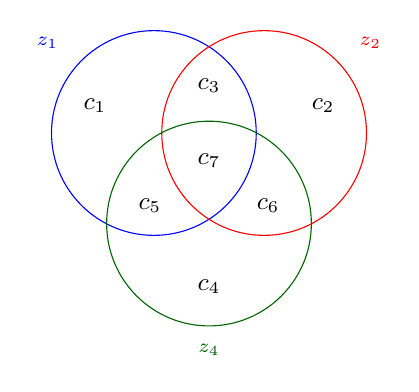
\begin{tikzpicture}[x=1cm,y=1cm]
	\draw[thin,color=blue]  (-0.7,0.4) circle (1.3);
	\draw[thin,color=red]   (0.7,0.4) circle (1.3);
	\draw[thin,color=DarkGreen] (0,-0.75) circle (1.3);
	\node[font=\small] at (-1.45,0.75) {$c_1$};
	\node[font=\small] at (1.45,0.75)  {$c_2$};
	\node[font=\small] at (0,-1.55)    {$c_4$};
	\node[font=\small] at (0,1.0)      {$c_3$};
	\node[font=\small] at (-0.75,-0.52){$c_5$};
	\node[font=\small] at (0.75,-0.52) {$c_6$};
	\node[font=\small] at (0,0.05)     {$c_7$};
	\node[font=\scriptsize,color=blue] at (-2.05,1.55) {$z_1$};
	\node[font=\scriptsize,color=red] at (2.05,1.55) {$z_2$};
	\node[font=\scriptsize,color=DarkGreen] at (0,-2.35) {$z_4$};
\end{tikzpicture}
\end{center}

Each circle must contain an even number of $1$s: those are exactly the three parity conditions
$$c_1+c_3+c_5+c_7 = 0,\quad c_2+c_3+c_6+c_7=0,\quad c_4+c_5+c_6+c_7=0.$$
Now the decoding rule becomes visual. A single error breaks precisely the parity of those circles containing it, and since every region is determined by the set of circles containing it, the broken circles identify the erroneous digit uniquely. If, for instance, only the blue and green circles fail, the culprit is $c_5$, which lies in those two and no other.

\subsection{Weight Enumerators}

The weights of the codewords of a linear code contain a great deal of information, and it is convenient to package them into a polynomial.

\begin{definition}[Weight Enumerator]
	The \vocab{weight enumerator} of a linear code $C \le \F_2^n$ is the homogeneous polynomial
	$$W_C(x,y) = \sum_{c \in C} x^{\,n-\wt(c)}y^{\,\wt(c)} = \sum_{i=0}^n A_i\, x^{n-i}y^i,$$
	where $A_i$ is the number of codewords of weight $i$.
\end{definition}

Note $W_C(1,1) = \abs{C}$ and $W_C(1,0) = 1$, and that $d(C)$ is the least $i>0$ with $A_i \ne 0$. If $C$ is used over a BSC with error probability $p$, then the probability that a transmitted codeword is received as another codeword -- an undetected error -- is $W_C(1-p,p) - (1-p)^n$, so the weight enumerator is exactly what one needs to analyse error detection.

\begin{example}
	The repetition code of length $n$ has $W(x,y) = x^n + y^n$. The simple parity check code of length $n$ has $W(x,y) = \sum_{i \text{ even}}\binom ni x^{n-i}y^i = \tfrac12\bigl[(x+y)^n + (x-y)^n\bigr]$. Hamming's $(7,4,3)$-code has weight distribution $A_0 = 1$, $A_3 = A_4 = 7$, $A_7 = 1$, so
	$$W(x,y) = x^7 + 7x^4y^3+7x^3y^4+y^7.$$
	(One checks $A_3 = 7$ directly: a weight-$3$ codeword corresponds to a triple of columns of $H$ summing to zero, and each of the $7$ nonzero syndromes $u$ determines such a triple. The remaining counts follow since $C$ contains $1111111$, so $A_i = A_{7-i}$.)
\end{example}

There is a beautiful and useful relation between the weight enumerator of a code and that of its dual, which comes from Fourier analysis on $\F_2^n$.

\begin{lemma}[Poisson Summation]\label{lem:poisson}
	Let $C \le \F_2^n$ be linear and let $f\colon \F_2^n \to \R$ have Fourier transform
	$$\hat f(v) = \sum_{u \in \F_2^n}(-1)^{u\cdot v}f(u).$$
	Then
	$$\sum_{v \in C}\hat f(v) = \abs{C}\sum_{u \in C^\perp}f(u).$$
\end{lemma}

\begin{proof}
	Exchanging the order of summation,
	$$\sum_{v\in C}\hat f(v) = \sum_{v\in C}\sum_{u}(-1)^{u\cdot v}f(u) = \sum_u f(u)\sum_{v\in C}(-1)^{u\cdot v}.$$
	The inner sum is $\abs{C}$ if $u \in C^\perp$. Otherwise the map $v \mapsto u\cdot v$ is a surjective linear map $C \to \F_2$, so its kernel has index $2$ in $C$ and the sum is $\tfrac12\abs{C} - \tfrac12\abs{C} = 0$.
\end{proof}

\begin{theorem}[MacWilliams Identity]
	For a linear code $C \le \F_2^n$,
	$$W_{C^\perp}(x,y) = \frac{1}{\abs{C}}\,W_C(x+y,\,x-y).$$
\end{theorem}

\begin{proof}
	Apply Lemma~\ref{lem:poisson} to $f(u) = x^{n-\wt(u)}y^{\wt(u)}$, which factorises as $f(u) = \prod_{i=1}^n g(u_i)$ with $g(0)=x$, $g(1)=y$. Then the Fourier transform factorises too:
	$$\hat f(v) = \sum_{u\in\F_2^n}\prod_{i=1}^n(-1)^{u_iv_i}g(u_i) = \prod_{i=1}^n\Bigl(\sum_{u_i \in \F_2}(-1)^{u_iv_i}g(u_i)\Bigr) = \prod_{i=1}^n\bigl(x+(-1)^{v_i}y\bigr),$$
	which is $(x+y)^{n-\wt(v)}(x-y)^{\wt(v)}$. Summing over $v \in C$ gives $W_C(x+y,x-y)$ on the left of Lemma~\ref{lem:poisson}, and $\abs{C}\,W_{C^\perp}(x,y)$ on the right.
\end{proof}

\begin{example}
	Take $C$ the simple parity check code of length $n$, with $W_C(x,y) = \tfrac12[(x+y)^n+(x-y)^n]$ and $\abs{C}=2^{n-1}$. Then
	$$W_{C^\perp}(x,y) = \frac{1}{2^{n-1}}\cdot\frac12\bigl[(2x)^n + (2y)^n\bigr] = x^n+y^n,$$
	which is the weight enumerator of the repetition code. And indeed the dual of the parity check code is the repetition code, as one sees directly.
\end{example}

\subsection{Reed--Muller Codes}

Our final family of linear codes is built out of the geometry of $\F_2^d$, and includes several codes we have already met. It is the family used by NASA to transmit the Mariner photographs of Mars.

Let $X = \{p_1,\dots,p_n\}$ be a set of size $n$. There is a chain of bijections
$$\power(X) \xrightarrow{\ A \mapsto \ii_A\ } \{f\colon X \to \F_2\} \xrightarrow{\ f \mapsto (f(p_1),\dots,f(p_n))\ } \F_2^n,$$
under which the symmetric difference $A \triangle B$ corresponds to vector addition, and the intersection $A \cap B$ corresponds to the \vocab{wedge product}
$$x \wedge y = (x_1y_1,\dots,x_ny_n).$$
So we may think of vectors in $\F_2^n$ as subsets of $X$, and we shall pass between the two pictures freely.

Now take $X = \F_2^d$, so that $n = \abs{X} = 2^d$. Let $v_0 = (1,1,\dots,1) = \ii_X$, and for $1 \le i \le d$ let
$$v_i = \ii_{H_i}, \qquad H_i = \{p \in X : p_i = 0\},$$
the indicator of the $i$th coordinate hyperplane.

\begin{definition}[Reed--Muller Code]
	For $0 \le r \le d$, the \vocab{Reed--Muller code} $RM(d,r)$ of \vocab{order} $r$ and length $2^d$ is the linear code spanned by $v_0$ together with all wedge products of at most $r$ of the $v_i$, $1 \le i \le d$. (By convention the empty wedge product is $v_0$.)
\end{definition}

\begin{example}\label{ex:rm3}
	Let $d = 3$ and list $X = \F_2^3$ in binary order. Then the spanning vectors are
	$$\begin{array}{c|cccccccc}
		X & 000&001&010&011&100&101&110&111\\\hline
		v_0 & 1&1&1&1&1&1&1&1\\
		v_1 & 1&1&1&1&0&0&0&0\\
		v_2 & 1&1&0&0&1&1&0&0\\
		v_3 & 1&0&1&0&1&0&1&0\\
		v_1\wedge v_2 & 1&1&0&0&0&0&0&0\\
		v_1\wedge v_3 & 1&0&1&0&0&0&0&0\\
		v_2\wedge v_3 & 1&0&0&0&1&0&0&0\\
		v_1\wedge v_2\wedge v_3 & 1&0&0&0&0&0&0&0
	\end{array}$$
	Notice that deleting the first column and keeping only the rows $v_0, v_1, v_2, v_3$ leaves a $4\times7$ matrix, and the code it generates has weight distribution $A_0 = 1$, $A_3 = A_4 = 7$, $A_7 = 1$. So it is a $(7,4,3)$-code -- indeed it is Hamming's original code, punctured out of $RM(3,1)$.
\end{example}

We can identify the small cases directly. $RM(3,0)$ is spanned by $v_0$ alone, so it is the repetition code of length $8$. $RM(3,1)$ is spanned by $v_0,v_1,v_2,v_3$, and is equivalent to the parity check extension of Hamming's $(7,4)$-code. $RM(3,2)$ is an $(8,7)$-code, equivalent to the simple parity check code of length $8$. And $RM(3,3)$ is the whole of $\F_2^8$.

\begin{theorem}\label{thm:rmrank}
	\begin{enumerate}[label=(\roman*)]
		\item The $2^d$ vectors $v_{i_1}\wedge\dots\wedge v_{i_s}$ with $i_1<\dots<i_s$ and $0 \le s \le d$ form a basis of $\F_2^n$, where $n = 2^d$.
		\item $\rank RM(d,r) = \sum_{s=0}^r \binom ds$.
	\end{enumerate}
\end{theorem}

\begin{proof}
	\emph{(i).} There are $\sum_{s=0}^d\binom ds = 2^d = n$ vectors in the list, so it suffices to show they span, that is, that $RM(d,d) = \F_2^n$. Fix $p \in X$ and set
	$$y_i = \begin{cases} v_i & \text{if } p_i = 0,\\ v_0+v_i & \text{if } p_i = 1.\end{cases}$$
	In the set picture $y_i$ is the indicator of $\{q : q_i = p_i\}$, so
	$$y_1 \wedge \dots \wedge y_d = \ii_{\{p\}}.$$
	Expanding the left hand side by distributivity of $\wedge$ over $+$ writes $\ii_{\{p\}}$ as a sum of wedge products of the $v_i$, hence $\ii_{\{p\}} \in RM(d,d)$. As $p$ was arbitrary and the $\ii_{\{p\}}$ span $\F_2^n$, we are done.

	\emph{(ii).} $RM(d,r)$ is spanned by those basis vectors with $s \le r$, of which there are $\sum_{s\le r}\binom ds$, and these are linearly independent by (i).
\end{proof}

To compute the minimum distance we use a construction which is of independent interest.

\begin{definition}[Bar Product]
	Let $C_2 \subseteq C_1$ be linear codes of length $n$. Their \vocab{bar product} is
	$$C_1 \mid C_2 = \{(x \mid x+y) : x \in C_1,\ y \in C_2\},$$
	a linear code of length $2n$.
\end{definition}

\begin{lemma}\label{lem:barprod}
	\begin{enumerate}[label=(\roman*)]
		\item $\rank(C_1\mid C_2) = \rank C_1 + \rank C_2$;
		\item $d(C_1\mid C_2) = \min\{2\,d(C_1),\ d(C_2)\}$.
	\end{enumerate}
\end{lemma}

\begin{proof}
	\emph{(i).} If $x_1,\dots,x_k$ is a basis of $C_1$ and $y_1,\dots,y_\ell$ a basis of $C_2$, then
	$$\{(x_i\mid x_i) : i \le k\}\cup\{(0\mid y_j): j\le\ell\}$$
	spans $C_1\mid C_2$, and is independent: a vanishing combination must have zero first half, forcing all $x$-coefficients to vanish, and then the $y$-coefficients too.

	\emph{(ii).} Let $(x\mid x+y)$ be a nonzero element. If $y \ne 0$ then, since weight is subadditive and $\wt(u)+\wt(u+v)\ge\wt(v)$,
	$$\wt(x\mid x+y) = \wt(x)+\wt(x+y)\ge \wt(y)\ge d(C_2).$$
	If $y = 0$ then $x \ne 0$ and $\wt(x\mid x) = 2\wt(x)\ge 2d(C_1)$. Hence $d(C_1\mid C_2)\ge\min\{2d(C_1),d(C_2)\}$. For the reverse, choose $x\in C_1$ of weight $d(C_1)$ to get a codeword $(x\mid x)$ of weight $2d(C_1)$, and choose $y \in C_2$ of weight $d(C_2)$ to get $(0 \mid y)$ of weight $d(C_2)$.
\end{proof}

\begin{theorem}\label{thm:rmdist}
	\begin{enumerate}[label=(\roman*)]
		\item $RM(d,r) = RM(d-1,r)\mid RM(d-1,r-1)$ for $0 < r< d$;
		\item $RM(d,r)$ has minimum distance $2^{d-r}$.
	\end{enumerate}
\end{theorem}

\begin{proof}
	\emph{(i).} Order $X = \F_2^d$ so that the points with last coordinate $0$ come first, identifying the two halves with $\F_2^{d-1}$. Under this splitting, the vectors $v_0,v_1,\dots,v_{d-1}$ for $\F_2^d$ become $(w\mid w)$ where $w$ is the corresponding vector for $\F_2^{d-1}$, while $v_d = (\mathbf{1}\mid \mathbf 0)$. A wedge product of at most $r$ of the $v_i$ with $i<d$ therefore has the form $(w\mid w)$ with $w \in RM(d-1,r)$; and a wedge product involving $v_d$ has the form $(w\mid 0)$ with $w \in RM(d-1,r-1)$, since one of its $r$ factors has been used up. As $(w \mid 0) = (w \mid w + w)$, every generator lies in $RM(d-1,r)\mid RM(d-1,r-1)$; and comparing ranks using Theorem~\ref{thm:rmrank}(ii), Lemma~\ref{lem:barprod}(i) and Pascal's rule
	$$\sum_{s\le r}\binom ds = \sum_{s \le r}\binom{d-1}{s} + \sum_{s\le r-1}\binom{d-1}{s}$$
	shows the two codes have the same dimension, hence are equal.

	\emph{(ii).} If $r=0$ then $RM(d,0)$ is the repetition code of length $2^d$, of minimum distance $2^d$. If $r=d$ then $RM(d,d) = \F_2^{2^d}$, of minimum distance $1 = 2^{d-d}$. For $0<r<d$ we induct on $d$, using (i) and Lemma~\ref{lem:barprod}(ii):
	$$d\bigl(RM(d,r)\bigr) = \min\{2\cdot2^{(d-1)-r},\ 2^{(d-1)-(r-1)}\} = \min\{2^{d-r},2^{d-r}\} = 2^{d-r}. \qedhere$$
\end{proof}

\begin{example}
	$RM(5,1)$ is a $(32,6)$-code with minimum distance $2^4 = 16$, so it corrects $7$ errors at rate $\frac6{32}$. This is the code used by Mariner 9 in 1971 to send back pictures of Mars: each pixel was one of $64$ grey levels, encoded in $32$ bits, and the channel was extremely noisy.
\end{example}


\section{Cyclic Codes}\label{sec:cyclic}

Linear codes made decoding into linear algebra. Imposing one further symmetry -- invariance under cyclic shifts -- turns them into ideals in a polynomial ring, and then all of the theory of finite fields from IB Groups, Rings and Modules comes into play. The reward is a family of codes with prescribed minimum distance and an efficient decoding algorithm.

\subsection{Cyclic Codes and Generator Polynomials}

\begin{definition}[Cyclic Code]
	A linear code $C \subseteq \F_2^n$ is \vocab{cyclic} if
	$$(a_0,a_1,\dots,a_{n-1}) \in C \implies (a_{n-1},a_0,\dots,a_{n-2}) \in C.$$
\end{definition}

Identify $\F_2^n$ with the quotient ring
$$R = \F_2[X]/(X^n-1)$$
via $\pi(a_0+a_1X+\dots+a_{n-1}X^{n-1}) = (a_0,\dots,a_{n-1})$; this is a bijection because every class modulo $X^n - 1$ has a unique representative of degree less than $n$. Under this identification, cyclic shift becomes multiplication by $X$:
$$X\cdot(a_0+a_1X+\dots+a_{n-1}X^{n-1}) = a_{n-1}+a_0X+\dots+a_{n-2}X^{n-1} \pmod{X^n-1}.$$

\begin{lemma}
	A code $C \subseteq \F_2^n$ is cyclic if and only if the corresponding subset $\Cc \subseteq R$ is an ideal of $R$.
\end{lemma}

\begin{proof}
	Linearity of $C$ says exactly that $\Cc$ is an additive subgroup, and the computation above says that closure under cyclic shift is closure under multiplication by $X$. Since $\Cc$ is closed under addition and multiplication by $X$, it is closed under multiplication by every polynomial, that is, it is an ideal; and conversely.
\end{proof}

From now on we identify $C$ with $\Cc$. Ideals of $R = \F_2[X]/(X^n-1)$ correspond to ideals of $\F_2[X]$ containing $X^n-1$; and $\F_2[X]$ is a principal ideal domain, so these correspond to the divisors of $X^n - 1$. This gives a complete classification.

\begin{theorem}[Generator Polynomial]\label{thm:genpoly}
	Let $C$ be a cyclic code of length $n$. Then there is a unique polynomial $g(X) \in \F_2[X]$ with
	\begin{enumerate}[label=(\roman*)]
		\item $C = (g)$, the ideal generated by $g$;
		\item $g(X) \mid X^n-1$.
	\end{enumerate}
	In particular, $p(X)$ represents a codeword if and only if $g \mid p$. We call $g$ the \vocab{generator polynomial} of $C$.
\end{theorem}

\begin{proof}
	Assume $C \ne \{0\}$ and let $g$ be a nonzero polynomial of least degree representing a codeword, so $\deg g < n$. Certainly $(g) \subseteq C$ since $C$ is an ideal. Conversely let $p$ represent a codeword; by the division algorithm in $\F_2[X]$, $p = qg+r$ with $\deg r< \deg g$. Then $r = p - qg \in C$, and minimality of $\deg g$ forces $r=0$. So $C = (g)$. Taking $p = X^n-1$, which represents $0 \in C$, gives $g \mid X^n-1$, which is (ii).

	For uniqueness, if $(g_1) = (g_2)$ then $g_1 \mid g_2$ and $g_2 \mid g_1$ in $\F_2[X]$ (using the divisibility of $X^n-1$ to work in $\F_2[X]$ rather than the quotient), so $g_1 = cg_2$ with $c \in \F_2^\times = \{1\}$.
\end{proof}

\begin{lemma}\label{lem:cyclicbasis}
	Let $C$ be cyclic of length $n$ with generator polynomial $g(X) = a_0+a_1X+\dots+a_kX^k$, $a_k \ne 0$. Then
	$$g,\ Xg,\ X^2g,\ \dots,\ X^{n-k-1}g$$
	is a basis for $C$, so $\rank C = n-k$.
\end{lemma}

\begin{proof}
	These $n-k$ polynomials have degrees $k, k+1, \dots, n-1$, all less than $n$, so they are genuine representatives and are linearly independent (distinct leading terms). They span: any codeword is $qg$ for some $q$, and reducing $q$ modulo $X^{n-k}$ we may assume $\deg q < n-k$, so $qg$ is a combination of the listed elements.
\end{proof}

\begin{corollary}
	With $g$ as above, a generator matrix for $C$ is the $(n-k)\times n$ matrix
	$$G = \begin{pmatrix}
		a_0 & a_1 & \cdots & a_k & 0 & \cdots & 0\\
		0 & a_0 & \cdots & a_{k-1} & a_k & \cdots & 0\\
		\vdots & & \ddots & & & \ddots & \vdots\\
		0 & 0 & \cdots & a_0 & a_1 & \cdots & a_k
	\end{pmatrix}.$$
\end{corollary}

\begin{definition}[Parity Check Polynomial]
	Let $g$ be the generator polynomial of a cyclic code $C$ of length $n$. The \vocab{parity check polynomial} is the polynomial $h$ with $g(X)h(X) = X^n-1$.
\end{definition}

\begin{corollary}
	Writing $h(X) = b_0+b_1X+\dots+b_{n-k}X^{n-k}$, a parity check matrix for $C$ is the $k\times n$ matrix
	$$H = \begin{pmatrix}
		b_{n-k} & b_{n-k-1} & \cdots & b_0 & 0 & \cdots & 0\\
		0 & b_{n-k} & \cdots & b_1 & b_0 & \cdots & 0\\
		\vdots & & \ddots & & & \ddots & \vdots\\
		0 & 0 & \cdots & b_{n-k} & b_{n-k-1} & \cdots & b_0
	\end{pmatrix}.$$
\end{corollary}

\begin{proof}
	The inner product of the $i$th row of $G$ with the $j$th row of $H$ is the coefficient of $X^{n-k-i+j}$ in $g(X)h(X) = X^n-1$. Since $1 \le i \le n-k$ and $1 \le j \le k$, we have $0 < n-k-i+j< n$, and all such coefficients of $X^n-1$ vanish. So the rows of $H$ lie in $C^\perp$; and $b_{n-k}\ne0$ gives $\rank H = k = \rank C^\perp$.
\end{proof}

\begin{remark}
	For $f(X) = \sum_{i=0}^m f_iX^i$ of degree $m$, the \vocab{reverse} polynomial is
	$$\check f(X) = f_m + f_{m-1}X+\dots+f_0X^m = X^mf(1/X).$$
	The matrix $H$ above is exactly the generator matrix built from $\check h$, so the dual of a cyclic code is the cyclic code generated by $\check h$. In particular the dual of a cyclic code is cyclic.
\end{remark}

\begin{lemma}\label{lem:squarefree}
	If $n$ is odd then $X^n-1 = f_1(X)\cdots f_t(X)$ with the $f_i$ distinct irreducible polynomials in $\F_2[X]$. Consequently there are exactly $2^t$ cyclic codes of length $n$.
\end{lemma}

\begin{proof}[Proof sketch]
	$X^n-1$ and its formal derivative $nX^{n-1} = X^{n-1}$ (as $n$ is odd) are coprime, so $X^n-1$ is separable and hence has no repeated irreducible factors. The cyclic codes correspond to the divisors of $X^n-1$, of which there are $2^t$.
\end{proof}

The hypothesis is needed: over $\F_2$ we have $X^2-1 = (X-1)^2$. From now on $n$ is odd.

\subsection{BCH Codes}

We now recall what we need about finite fields, all of which is from IB Groups, Rings and Modules. If $f \in \F_p[X]$ is irreducible then $\F_p[X]/(f)$ is a field with $p^{\deg f}$ elements, and every finite field arises this way; for each prime power $q = p^\alpha$ there is a unique field $\F_q$ of order $q$ up to isomorphism (note $\F_q \not\cong \Z/q\Z$ when $\alpha>1$). The multiplicative group $\F_q^\times$ is cyclic of order $q-1$, and a generator is called a \vocab{primitive element}.

Fix an odd $n$, and choose $r \ge 1$ with $2^r \equiv 1 \pmod n$; such $r$ exists since $2$ is a unit modulo $n$. Let $K = \F_{2^r}$ and set
$$\mu_n(K) = \{x \in K : x^n = 1\} \le K^\times.$$
As $n \mid 2^r-1 = \abs{K^\times}$ and $K^\times$ is cyclic, $\mu_n(K)$ is cyclic of order exactly $n$, say
$$\mu_n(K) = \{1,\alpha,\alpha^2,\dots,\alpha^{n-1}\}$$
for a primitive $n$th root of unity $\alpha \in K$. Since $n$ is odd, $X^n-1$ has $n$ distinct roots in $K$, namely these, so $K$ contains a splitting field for $X^n-1$.

\begin{definition}[Defining Set]
	Let $A \subseteq \mu_n(K)$. The cyclic code of length $n$ with \vocab{defining set} $A$ is
	$$C = \bigl\{f(X) \in \F_2[X]/(X^n-1) : f(a) = 0 \text{ for all } a \in A\bigr\}.$$
\end{definition}

This really is cyclic: the conditions $f(a)=0$ are $\F_2$-linear and are preserved under multiplication by $X$. Its generator polynomial is the nonzero polynomial in $\F_2[X]$ of least degree vanishing on $A$, that is, the least common multiple of the minimal polynomials over $\F_2$ of the elements of $A$.

\begin{definition}[BCH Code]
	The cyclic code of length $n$ with defining set $\{\alpha,\alpha^2,\dots,\alpha^{\delta-1}\}$ is the \vocab{BCH code} with \vocab{design distance} $\delta$. (The name is for Bose, Ray-Chaudhuri and Hocquenghem.)
\end{definition}

The point of the definition is the following bound, which lets us specify the minimum distance in advance -- something no construction so far has allowed.

\begin{lemma}[Vandermonde]\label{lem:vandermonde}
	$$\det\begin{pmatrix}
		1 & 1 & \cdots & 1\\
		x_1 & x_2 & \cdots & x_n\\
		\vdots & \vdots & \ddots & \vdots\\
		x_1^{n-1} & x_2^{n-1} & \cdots & x_n^{n-1}
	\end{pmatrix} = \prod_{1\le j<i\le n}(x_i-x_j).$$
	In particular the determinant is nonzero whenever the $x_i$ are distinct.
\end{lemma}

\begin{theorem}[BCH Bound]
	A BCH code $C$ with design distance $\delta$ has $d(C)\ge\delta$.
\end{theorem}

\begin{proof}
	Consider the $(\delta-1)\times n$ matrix over $K$
	$$H = \begin{pmatrix}
		1 & \alpha & \alpha^2 & \cdots & \alpha^{n-1}\\
		1 & \alpha^2 & \alpha^4 & \cdots & \alpha^{2(n-1)}\\
		\vdots & \vdots & \vdots & \ddots & \vdots\\
		1 & \alpha^{\delta-1} & \alpha^{2(\delta-1)} & \cdots & \alpha^{(\delta-1)(n-1)}
	\end{pmatrix}.$$
	A word $c \in \F_2^n$ lies in $C$ precisely when $Hc = 0$, since the $j$th row of $Hc$ is $c(\alpha^j)$. Take any $\delta-1$ columns of $H$, say those indexed by $i_1<\dots<i_{\delta-1}$. Dividing the $j$th row by nothing and factoring $\alpha^{i_s}$ out of the $s$th column, the resulting $(\delta-1)\times(\delta-1)$ matrix is a Vandermonde matrix in the distinct elements $\alpha^{i_1},\dots,\alpha^{i_{\delta-1}}$, hence invertible by Lemma~\ref{lem:vandermonde}. So no $\delta-1$ columns of $H$ are linearly dependent, and by the argument of Lemma~\ref{lem:distH} every nonzero codeword has weight at least $\delta$.
\end{proof}

\begin{remark}
	The matrix $H$ is not a parity check matrix in our earlier sense, since its entries lie in $K$ rather than $\F_2$. Nevertheless the dependence argument goes through verbatim, because a codeword is a vector over $\F_2 \subseteq K$ and linear dependence over $K$ is what we tested.
\end{remark}

\begin{example}\label{ex:bch7}
	Take $n = 7$. Over $\F_2$,
	$$X^7-1 = (X+1)(X^3+X+1)(X^3+X^2+1),$$
	so by Lemma~\ref{lem:squarefree} there are $2^3 = 8$ cyclic codes of length $7$. Take $g(X) = X^3+X+1$, so
	$$h(X) = (X+1)(X^3+X^2+1) = X^4+X^2+X+1,$$
	and $\rank C = 7 - 3 = 4$. The parity check matrix built from $\check h(X) = X^4 + X^3 + X^2 + 1$ is
	$$H = \begin{pmatrix} 1&0&1&1&1&0&0\\0&1&0&1&1&1&0\\0&0&1&0&1&1&1\end{pmatrix},$$
	whose columns are precisely the seven nonzero elements of $\F_2^3$. So $C$ is (equivalent to) the Hamming $(7,4)$-code.

	Let us see this again from the BCH point of view. Take $K = \F_8 = \F_2[\beta]/(\beta^3+\beta+1)$, so $\beta$ is a root of $g$ and a primitive $7$th root of unity. The powers of $\beta$ are
	$$\begin{array}{c|ccccccc}
		i & 0&1&2&3&4&5&6\\\hline
		\beta^i & 1 & \beta & \beta^2 & \beta+1 & \beta^2+\beta & \beta^2+\beta+1 & \beta^2+1
	\end{array}$$
	Squaring is a field automorphism of $K$ fixing $\F_2$, so $g(\beta) = 0$ gives $g(\beta^2) = g(\beta)^2 = 0$ and likewise $g(\beta^4)=0$. Hence the BCH code with defining set $\{\beta,\beta^2\}$ has generator polynomial exactly $g$, and its design distance is $\delta = 3$. So $d(C)\ge3$; and we know Hamming's code has $d = 3$ exactly.
\end{example}

\subsection{Decoding BCH Codes}

Let $C$ be a BCH code of length $n$ with defining set $\{\alpha,\dots,\alpha^{\delta-1}\}$, so $d(C)\ge\delta$ and $C$ should correct
$$t = \floor{\frac{\delta-1}{2}}$$
errors. Suppose $c \in C$ is sent and $r = c+e$ is received, where the error pattern $e$ has at most $t$ nonzero digits. Writing $r(X), c(X), e(X)$ for the corresponding polynomials, $c(\alpha^j)=0$ for $1\le j\le\delta-1$ and so
$$r(\alpha^j) = e(\alpha^j), \qquad 1 \le j \le \delta-1.$$
These $\delta-1$ elements of $K$ are the \vocab{syndromes}, and everything must be recovered from them.

\begin{definition}[Error Locator Polynomial]
	Let $\Ec = \{i : e_i = 1\}$ be the set of error positions. The \vocab{error locator polynomial} is
	$$\sigma(X) = \prod_{i\in\Ec}\bigl(1-\alpha^iX\bigr) \in K[X].$$
\end{definition}

The roots of $\sigma$ are exactly the $\alpha^{-i}$ for $i \in \Ec$, so knowing $\sigma$ is the same as knowing where the errors are. Note $\sigma(0)=1$ and $\deg\sigma = \abs{\Ec} \le t$.

\begin{theorem}\label{thm:errorlocator}
	Suppose $\abs{\Ec}\le t$ where $2t+1\le\delta$. Then $\sigma(X)$ is the unique polynomial of least degree in $K[X]$ such that
	\begin{enumerate}[label=(\roman*)]
		\item $\sigma(0) = 1$;
		\item $\displaystyle \sigma(X)\sum_{j=1}^{2t}r(\alpha^j)X^j \equiv \omega(X) \pmod{X^{2t+1}}$ for some $\omega \in K[X]$ with $\deg\omega\le t$.
	\end{enumerate}
\end{theorem}

\begin{proof}
	\emph{Existence.} Define the \vocab{error co-locator} $\omega(X) = -X\sigma'(X)$, so by the product rule
	$$\omega(X) = \sum_{i\in\Ec}\alpha^iX\prod_{j\in\Ec,\, j\ne i}(1-\alpha^jX),$$
	which has degree $\deg \sigma = \abs{\Ec}\le t$. Work in the ring $K[[X]]$ of formal power series, in which $1-\alpha^iX$ is invertible. A partial fractions computation gives
	$$\frac{\omega(X)}{\sigma(X)} = \sum_{i\in\Ec}\frac{\alpha^iX}{1-\alpha^iX} = \sum_{i\in\Ec}\sum_{j\ge1}(\alpha^iX)^j = \sum_{j\ge1}X^j\sum_{i\in\Ec}(\alpha^j)^i = \sum_{j\ge1}e(\alpha^j)X^j,$$
	the last step because $e(X) = \sum_{i\in\Ec}X^i$. Hence
	$$\sigma(X)\sum_{j\ge1}e(\alpha^j)X^j = \omega(X)$$
	exactly, in $K[[X]]$. Since $2t \le \delta-1$ we have $r(\alpha^j)=e(\alpha^j)$ for $1 \le j\le 2t$, and truncating modulo $X^{2t+1}$ gives (ii).

	\emph{Uniqueness.} Suppose $\widetilde\sigma,\widetilde\omega$ also satisfy (i) and (ii) with $\deg\widetilde\sigma\le\deg\sigma$. The roots of $\sigma$ are distinct and nonzero, and $\omega(X) = -X\sigma'(X)$ does not vanish at them (differentiate $\sigma$ at a simple root); so $\sigma$ and $\omega$ are coprime. From (ii) for both pairs,
	$$\widetilde\sigma(X)\omega(X)\equiv\sigma(X)\widetilde\omega(X) \pmod{X^{2t+1}},$$
	and both sides have degree at most $2t$, so this is an equality of polynomials. Since $\sigma$ and $\omega$ are coprime, $\sigma\mid\widetilde\sigma$; combined with $\deg\widetilde\sigma\le\deg\sigma$ this gives $\widetilde\sigma = \lambda\sigma$, and (i) forces $\lambda = 1$.
\end{proof}

This yields an algorithm. On receiving $r(X)$:
\begin{enumerate}[label=(\arabic*)]
	\item Compute the syndromes $r(\alpha^j)$ for $1 \le j \le 2t$ and form $S(X) = \sum_{j=1}^{2t}r(\alpha^j)X^j$.
	\item Write $\sigma(X) = 1 + \sigma_1X+\dots+\sigma_tX^t$ with unknown coefficients. Condition (ii) says the coefficients of $X^i$ in $\sigma(X)S(X)$ vanish for $t+1\le i\le 2t$, giving $t$ linear equations
	$$\sum_{j=0}^{t}\sigma_j\, r(\alpha^{i-j}) = 0, \qquad \sigma_0 = 1.$$
	\item Solve these over $K$, keeping a solution of least degree.
	\item Compute $\Ec = \{i : \sigma(\alpha^{-i}) = 0\}$ and check $\abs{\Ec} = \deg\sigma$.
	\item Set $e(X) = \sum_{i\in\Ec}X^i$, put $c(X) = r(X)+e(X)$, and check that $c$ is a codeword.
\end{enumerate}

\begin{example}
	Continue Example~\ref{ex:bch7}: $n = 7$, $g(X)=X^3+X+1$, defining set $\{\beta,\beta^2\}$, $\delta = 3$, $t = 1$. Take the codeword $c(X) = g(X) = 1+X+X^3$, that is $c = 1101000$, and suppose an error occurs in position $5$, so
	$$r(X) = 1+X+X^3+X^5.$$
	We compute the syndromes, using the table of powers of $\beta$ above:
	$$r(\beta) = 1+\beta+(\beta+1)+(\beta^2+\beta+1) = 1 + \beta+\beta^2 = \beta^5,$$
	and $r(\beta^2) = r(\beta)^2 = \beta^{10} = \beta^3$. So $S(X) = \beta^5X+\beta^3X^2$.

	With $t=1$ we set $\sigma(X) = 1+\sigma_1X$; the coefficient of $X^2$ in $\sigma(X)S(X)$ is $\beta^3 + \sigma_1\beta^5$, which must vanish, so
	$$\sigma_1 = \beta^{3-5} = \beta^{-2}=\beta^5.$$
	Thus $\sigma(X) = 1+\beta^5X$, whose root is $X = \beta^{-5} = \beta^2$. Solving $\beta^{-i} = \beta^2$ gives $i \equiv -2\equiv 5 \pmod 7$, so $\Ec = \{5\}$ and $\abs{\Ec}=1=\deg\sigma$ as required. Correcting, $c(X) = r(X)+X^5 = 1+X+X^3$, which is indeed a codeword. Everything is consistent.
\end{example}

\begin{example}
	For a code that genuinely corrects two errors, take $n = 15$ and $K = \F_{16} = \F_2[\alpha]/(\alpha^4+\alpha+1)$, so $\alpha$ is a primitive $15$th root of unity. The minimal polynomial of $\alpha$ is $X^4+X+1$ (with roots $\alpha,\alpha^2,\alpha^4,\alpha^8$) and that of $\alpha^3$ is $X^4+X^3+X^2+X+1$ (with roots $\alpha^3,\alpha^6,\alpha^{12},\alpha^9$). The BCH code with defining set $\{\alpha,\alpha^2,\alpha^3,\alpha^4\}$ therefore has
	$$g(X) = (X^4+X+1)(X^4+X^3+X^2+X+1)$$
	of degree $8$, giving a $(15,7)$-code with design distance $5$; in fact $d = 5$ exactly, so it is a $(15,7,5)$-code correcting two errors.
\end{example}

\subsection{Reed--Solomon Codes}

Everything above works over any finite field, and one particularly clean case deserves its own name. Let $q$ be a prime power, let $\alpha$ be a primitive element of $\F_q$, and take $n = q-1$, so that $\alpha$ is a primitive $n$th root of unity \emph{in the field $\F_q$ itself}. Codes are now subsets of $\F_q^n$; Hamming distance, weight and linearity all make sense verbatim.

\begin{definition}[Reed--Solomon Code]
	Let $1 \le k \le n = q-1$. The \vocab{Reed--Solomon code} $RS(n,k)$ is the cyclic code over $\F_q$ of length $n$ with generator polynomial
	$$g(X) = (X-\alpha)(X-\alpha^2)\cdots(X-\alpha^{n-k}).$$
\end{definition}

Equivalently it is the BCH code with defining set $\{\alpha,\dots,\alpha^{n-k}\}$ and design distance $\delta = n-k+1$; the difference from the binary case is that the defining set already consists of elements of the ground field, so no extension is needed and the degree of $g$ is exactly $n - k$.

\begin{proposition}
	$RS(n,k)$ has rank $k$ and minimum distance exactly $n-k+1$. In particular it is MDS: it attains the Singleton bound.
\end{proposition}

\begin{proof}
	Since $\deg g = n-k$, Lemma~\ref{lem:cyclicbasis} gives $\rank = n - (n-k) = k$. The BCH bound gives $d \ge \delta = n-k+1$, and the Singleton bound (Theorem~\ref{thm:singleton}, whose proof works over any alphabet, giving $\abs{C}\le q^{\,n-d+1}$) gives $q^k \le q^{\,n-d+1}$, that is, $d \le n-k+1$.
\end{proof}

\begin{example}
	Take $q = 5$ and $\alpha = 2$, a primitive root modulo $5$ since $2,4,3,1$ are its successive powers. With $n = 4$ and $k = 2$,
	$$g(X) = (X-2)(X-4) = X^2-6X+8 = X^2+4X+3 \in \F_5[X],$$
	and indeed $g \mid X^4-1 = (X-1)(X-2)(X-3)(X-4)$. The code is
	$$RS(4,2) = \{(a+bX)g(X) : a,b\in\F_5\},$$
	of size $25$. For instance $g$ itself is the codeword $(3,4,1,0)$, of weight $3$, and one checks that every nonzero codeword has weight at least $3 = n-k+1$. So this is a $(4,2,3)$ MDS code over $\F_5$.
\end{example}

\begin{remark}
	Reed--Solomon codes are ubiquitous in practice -- they are what protects the data on a compact disc, in a QR code, and on the Voyager spacecraft. Their great virtue is that a symbol of $\F_{2^m}$ is a block of $m$ bits, so a single symbol error absorbs a whole \emph{burst} of up to $m$ consecutive bit errors. Real channels tend to produce errors in bursts rather than independently, which is exactly the situation the binary symmetric channel fails to model.
\end{remark}

\subsection{Linear Feedback Shift Registers}

We now change tack, apparently completely, and consider a piece of hardware. The connection to what we have just done will emerge shortly, and it will also be the basis of the stream ciphers of Section~\ref{cc-sec:crypto}.

\begin{definition}[Feedback Shift Register]
	A \vocab{(general) feedback shift register} of length $d$ is a map $f\colon\F_2^d\to\F_2^d$ of the form
	$$f(x_0,\dots,x_{d-1}) = \bigl(x_1,\dots,x_{d-1},\,C(x_0,\dots,x_{d-1})\bigr)$$
	for some function $C\colon\F_2^d\to\F_2$. Given an \vocab{initial fill} $(y_0,\dots,y_{d-1})$, the associated \vocab{stream} is the sequence $y_0,y_1,\dots$ defined by
	$$y_n = C(y_{n-d},\dots,y_{n-1}), \qquad n \ge d.$$
\end{definition}

\begin{definition}[LFSR]
	A feedback shift register is a \vocab{linear feedback shift register} (LFSR) if $C$ is linear, say
	$$C(x_0,\dots,x_{d-1}) = \sum_{i=0}^{d-1}a_ix_i.$$
	We always take $a_0 = 1$, since otherwise the register really has length less than $d$.
\end{definition}

Physically it is a row of $d$ memory cells; at each tick every cell passes its contents to its left neighbour, the leftmost cell is output, and the rightmost cell receives the sum of the tapped cells.

\begin{center}
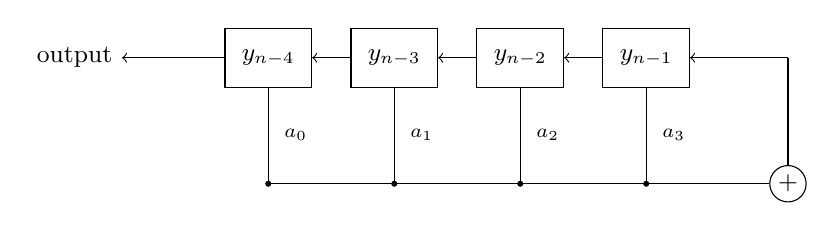
\begin{tikzpicture}[x=1cm,y=1cm]
	\tikzset{cell/.style={draw,thin,minimum width=1.1cm,minimum height=0.75cm,font=\small}}
	\node[cell] (c0) at (0,0)   {$y_{n-4}$};
	\node[cell] (c1) at (1.6,0) {$y_{n-3}$};
	\node[cell] (c2) at (3.2,0) {$y_{n-2}$};
	\node[cell] (c3) at (4.8,0) {$y_{n-1}$};
	\draw[->,thin] (c1.west) -- (c0.east);
	\draw[->,thin] (c2.west) -- (c1.east);
	\draw[->,thin] (c3.west) -- (c2.east);
	\draw[->,thin] (c0.west) -- ++(-1.3,0) node[left,font=\small] {output};
	\node[draw,circle,thin,inner sep=1.3pt,font=\small] (xor) at (6.6,-1.6) {$+$};
	\draw[thin] (0,-1.6) -- (xor.west);
	\foreach \x/\lab in {0/{a_0}, 1.6/{a_1}, 3.2/{a_2}, 4.8/{a_3}}{
		\draw[thin] (\x,-0.375) -- (\x,-1.6);
		\fill (\x,-1.6) circle (1.1pt);
		\node[font=\scriptsize,right] at (\x+0.08,-0.98) {$\lab$};
	}
	\draw[thin] (xor.north) -- (6.6,0);
	\draw[->,thin] (6.6,0) -- (c3.east);
\end{tikzpicture}
\end{center}

For an LFSR the stream satisfies the linear recurrence
$$y_n = \sum_{i=0}^{d-1}a_iy_{n-d+i}, \qquad n \ge d,$$
and it is natural to encode the coefficients in a polynomial.

\begin{definition}[Auxiliary and Feedback Polynomials]
	The \vocab{auxiliary polynomial} of the LFSR is
	$$P(X) = X^d + a_{d-1}X^{d-1}+\dots+a_1X+a_0 = \sum_{i=0}^d a_iX^i \quad (a_d := 1),$$
	and the \vocab{feedback polynomial} is its reverse
	$$\check P(X) = a_0X^d+a_1X^{d-1}+\dots+a_{d-1}X+1 = \sum_{i=0}^d a_{d-i}X^i.$$
	The \vocab{generating function} of a stream $(y_n)$ is $G(X) = \sum_{j\ge0}y_jX^j \in \F_2[[X]]$.
\end{definition}

\begin{theorem}\label{thm:lfsrgf}
	A stream $(y_n)_{n\ge0}$ arises from an LFSR with auxiliary polynomial $P$ if and only if its generating function has the form
	$$G(X) = \frac{A(X)}{\check P(X)}$$
	for some $A \in \F_2[X]$ with $\deg A < \deg\check P = d$.
\end{theorem}

\begin{proof}
	The condition is that
	$$G(X)\check P(X) = \Bigl(\sum_{j\ge0}y_jX^j\Bigr)\Bigl(\sum_{i=0}^d a_{d-i}X^i\Bigr)$$
	is a polynomial of degree less than $d$, that is, that the coefficient of $X^n$ vanishes for all $n \ge d$. That coefficient is
	$$\sum_{i=0}^d a_{d-i}y_{n-i} = y_n + \sum_{i=1}^{d}a_{d-i}y_{n-i},$$
	using $a_d = 1$. Setting this to zero and reindexing gives exactly $y_n = \sum_{i=0}^{d-1}a_iy_{n-d+i}$.
\end{proof}

So streams from LFSRs of length $d$ are precisely the sequences whose generating function is a rational function with denominator of degree $d$ -- which is the same problem we solved when decoding BCH codes, where we had to recognise a power series as $\omega/\sigma$. The two subjects are the same subject.

\begin{example}\label{ex:lfsr}
	Take $d = 4$ with $a_0 = a_1 = 1$ and $a_2=a_3=0$, so
	$$y_n = y_{n-4}+y_{n-3}, \qquad P(X) = X^4+X+1, \qquad \check P(X) = X^4+X^3+1.$$
	With initial fill $1000$ the stream begins
	$$1,0,0,0,1,0,0,1,1,0,1,0,1,1,1,\ 1,0,0,0,1,\dots$$
	and one checks that $y_{15+r} = y_r$, so the period is $15 = 2^4-1$, the largest possible. (This happens exactly when $P$ is a primitive polynomial, meaning that its roots are primitive elements of $\F_{16}$.)
\end{example}

\subsection{The Berlekamp--Massey Method}

Suppose now that we are handed a stream $(x_n)$ which we are told comes from \emph{some} LFSR, but we know neither its length $d$ nor its coefficients. Recovering them is the problem of \vocab{linear complexity}, and it has a clean linear-algebraic solution.

We seek $d$ and $a_0,\dots,a_{d-1}$ (with $a_d = 1$) such that
$$x_n + \sum_{i=1}^{d}a_{d-i}x_{n-i} = 0 \qquad \text{for all } n \ge d.$$
Writing out these equations for $n = d, d+1, \dots, 2d$ gives the matrix equation
$$\underbrace{\begin{pmatrix}
	x_d & x_{d-1} & \cdots & x_1 & x_0\\
	x_{d+1} & x_d & \cdots & x_2 & x_1\\
	\vdots & \vdots & \ddots & \vdots & \vdots\\
	x_{2d} & x_{2d-1} & \cdots & x_{d+1} & x_d
\end{pmatrix}}_{A_d}
\begin{pmatrix} a_d\\ a_{d-1}\\ \vdots \\ a_1 \\ a_0\end{pmatrix} = 0.$$
This is a system of $d+1$ homogeneous equations in $d+1$ unknowns, and it has a nonzero solution -- our sought-after coefficients, with $a_d = 1$ -- so $\det A_d = 0$.

The \vocab{Berlekamp--Massey method} exploits this. Compute $\det A_0, \det A_1, \det A_2, \dots$ in turn (starting at $A_r$ if we already know $d \ge r$).
\begin{itemize}
	\item If $\det A_i \ne 0$ then $d \ne i$, and we move on.
	\item If $\det A_i = 0$ we tentatively assume $d = i$, solve the system for $a_0,\dots,a_{i-1}$, and test the resulting recurrence against as many further terms of the stream as we like. If it fails, we move on.
\end{itemize}
The first $i$ that survives the test is the answer.

\begin{example}
	Apply this to the stream of Example~\ref{ex:lfsr}, pretending we do not know where it came from:
	$$x = 1,0,0,0,1,0,0,1,1,0,1,0,1,1,1,\dots$$
	\begin{itemize}
		\item $A_0 = \begin{pmatrix}x_0\end{pmatrix} = \begin{pmatrix}1\end{pmatrix}$ has $\det = 1 \ne 0$, so $d \ne 0$.
		\item $A_1 = \begin{pmatrix}x_1 & x_0\\ x_2 & x_1\end{pmatrix} = \begin{pmatrix}0&1\\0&0\end{pmatrix}$ has $\det = 0$. Solving with $a_1 = 1$: the first row gives $0\cdot1 + a_0 = 0$, so $a_0 = 0$, and the recurrence $x_n = 0$ fails already at $x_4 = 1$. So $d \ne 1$.
		\item $A_2 = \begin{pmatrix}0&0&1\\0&0&0\\1&0&0\end{pmatrix}$ has a zero row, so $\det = 0$. Solving with $a_2=1$: row $1$ gives $a_0 = 0$, row $3$ gives $x_4 + a_1x_3+a_0x_2 = 1 \ne 0$. The system is inconsistent, so $d\ne2$.
		\item $A_3 = \begin{pmatrix}0&0&0&1\\1&0&0&0\\0&1&0&0\\0&0&1&0\end{pmatrix}$ is a permutation matrix, so $\det = 1\ne0$ and $d \ne 3$.
		\item $A_4 = \begin{pmatrix}1&0&0&0&1\\0&1&0&0&0\\0&0&1&0&0\\1&0&0&1&0\\1&1&0&0&1\end{pmatrix}$. Solving with $a_4=1$: the rows give in turn $a_0 = 1$, $a_3 = 0$, $a_2 = 0$, $a_1 = 1$, and the last row $1+a_3+a_0 = 1+0+1 = 0$ is consistent. (So $\det A_4 = 0$, as it must be.)
	\end{itemize}
	We conclude that $d = 4$ with $(a_0,a_1,a_2,a_3) = (1,1,0,0)$, that is, $y_n = y_{n-4}+y_{n-3}$, which is exactly the register we started with. Checking against the later terms of the stream confirms it.
\end{example}

\begin{remark}
	The moral for cryptography is discouraging. A stream produced by a linear feedback shift register of length $d$ is completely determined by $2d$ of its terms, recoverable by solving a linear system. Any cipher whose key stream is generated linearly is therefore broken by a modest amount of known plaintext, as we shall see in Section~\ref{cc-sec:crypto}.
\end{remark}


\section{Cryptography}\label{cc-sec:crypto}

We now turn from noise to malice. Alice wants to send Bob a message, and Eve is listening. The techniques of the previous sections were designed against an opponent -- the channel -- who was random but not clever; now our opponent is clever, and we have to design against the worst case rather than the average one.

\subsection{Cryptosystems and Classical Ciphers}

Alice and Bob share some secret information called the \vocab{key}, drawn from a set $\Kc$. The unencrypted message, the \vocab{plaintext}, lies in a set $\Mc$, and the encrypted message, the \vocab{ciphertext}, lies in a set $\Cc$.

\begin{definition}[Cryptosystem]
	A \vocab{cryptosystem} consists of sets $(\Mc,\Kc,\Cc)$ together with an \vocab{encryption} function $e\colon\Mc\times\Kc\to\Cc$ and a \vocab{decryption} function $d\colon\Cc\times\Kc\to\Mc$ satisfying
	$$d\bigl(e(m,k),k\bigr) = m \qquad \text{for all } m \in \Mc,\ k \in \Kc.$$
\end{definition}

\begin{example}[Substitution and Vigen\`ere Ciphers]
	Let $\Sigma = \{A,B,\dots,Z\}$ and $\Mc = \Cc = \Sigma^\star$.
	\begin{itemize}
		\item The \vocab{simple substitution cipher} takes $\Kc$ to be the set of permutations of $\Sigma$; each plaintext letter is replaced by its image under the chosen $\pi \in \Kc$. There are $26! \approx 4\times10^{26}$ keys, which sounds like a lot.
		\item The \vocab{Vigen\`ere cipher} takes $\Kc = \Sigma^d$ for some $d$. Identify $\Sigma$ with $\Z/26\Z$, write the key repeatedly beneath the plaintext, and add. For instance, the plaintext \texttt{ATTACKATDAWN} with key \texttt{LEMON} gives
		$$\begin{array}{l}
		\texttt{ATTACKATDAWN}\\ \texttt{LEMONLEMONLE}\\\hline \texttt{LXFOPVEFRNHR}\end{array}$$
		The case $d = 1$ is the \vocab{Caesar cipher}.
	\end{itemize}
\end{example}

Neither of these is secure, and it is worth being precise about what security would mean. We assume throughout \vocab{Kerckhoffs' principle}: Eve knows the functions $e$ and $d$ and the probability distributions on $\Kc$ and $\Mc$; the only thing she does not know is the key itself. There is then a hierarchy of attacks.

\begin{enumerate}[label=\textbf{Level \arabic*.}, leftmargin=*]
	\item \emph{Ciphertext only.} Eve knows some ciphertext and nothing else.
	\item \emph{Known plaintext.} Eve knows a substantial stretch of plaintext together with its ciphertext, but not the key.
	\item \emph{Chosen plaintext.} Eve can obtain the ciphertext of any plaintext she likes.
\end{enumerate}

\begin{remark}
	Both examples above fail at Level 1 against English plaintext of any length, by frequency analysis: in the substitution cipher the letter frequencies are merely permuted, and in the Vigen\`ere cipher the same is true within each residue class modulo $d$ (and $d$ itself is found by looking for repeated ciphertext fragments). Even against random-looking plaintext, both fall immediately at Level 2, since a single plaintext--ciphertext pair reveals the key. Modern applications demand Level 3 security.
\end{remark}

\subsection{Perfect Secrecy and the One-Time Pad}

To do better we should say what perfect security means, and information theory gives us the language. Model the key and message as \emph{independent} random variables $K, M$ on $\Kc,\Mc$, and let $C = e(M,K)$ be the ciphertext.

\begin{definition}[Perfect Secrecy]
	A cryptosystem has \vocab{perfect secrecy} if $H(M\mid C) = H(M)$; equivalently $I(M;C)=0$; equivalently $M$ and $C$ are independent.
\end{definition}

In other words, seeing the ciphertext tells Eve nothing at all about the message that she did not already know. This is an extremely strong requirement, and it is expensive.

\begin{proposition}[Shannon]\label{prop:keylength}
	Suppose a cryptosystem has perfect secrecy, and that every message in $\Mc$ and every ciphertext in $\Cc$ occurs with positive probability. Then $\abs{\Kc}\ge\abs{\Cc}\ge\abs{\Mc}$. In particular the key is at least as long as the message.
\end{proposition}

\begin{proof}
	Fix a key $k$. The map $m \mapsto e(m,k)$ is injective, since $d(\cdot,k)$ inverts it; hence $\abs{\Cc}\ge\abs{\Mc}$.

	Now fix a ciphertext $c \in \Cc$ and a message $m \in \Mc$. By perfect secrecy $M$ and $C$ are independent, so
	$$\PP(C = c \mid M = m) = \PP(C = c) > 0,$$
	and therefore there is at least one key $k$ with $e(m,k) = c$. Fix $c$ and let $m$ range over $\Mc$: the keys so obtained are distinct, because a single key $k$ can satisfy $e(m,k) = c$ for at most one $m$, again by injectivity. Hence $\abs{\Kc}\ge\abs{\Mc}$. Applying the same argument with $m$ fixed and $c$ ranging over $\Cc$ -- for each $c$ there is a key carrying $m$ to $c$, and distinct $c$ need distinct keys since $e(m,\cdot)$ is a function -- gives $\abs{\Kc}\ge\abs{\Cc}$.
\end{proof}

So perfect secrecy demands a key space at least as large as the message space: a fresh $\log\abs{\Mc}$ bits of shared secret for every message sent. That is a heavy price, and we shall see at the end of this section that the one-time pad pays exactly it. Before that, it is worth quantifying how far short of perfection an imperfect system falls, and for that we need two more pieces of vocabulary.

\begin{definition}
	The \vocab{message equivocation} is $H(M\mid C)$ and the \vocab{key equivocation} is $H(K\mid C)$.
\end{definition}

\begin{lemma}
	$H(M\mid C)\le H(K\mid C)$.
\end{lemma}

\begin{proof}
	Since $M = d(C,K)$, knowing $C$ and $K$ determines $M$, so $H(M\mid C,K) = 0$ and hence $H(M,C,K) = H(C,K)$. Now expand by the chain rule in two ways:
	\begin{align*}
		H(K\mid C) &= H(K,C)-H(C) = H(M,C,K)-H(C)\\
		&= H(K\mid M,C) + H(M,C) - H(C) = H(K\mid M,C)+H(M\mid C),
	\end{align*}
	and $H(K\mid M,C)\ge0$.
\end{proof}

So determining the key is at least as hard as determining the message -- which is reassuring, since it means we may safely study the key equivocation instead.

Suppose $\Mc = \Cc = \Ac$ and we send $n$ messages $M^{(n)} = (M_1,\dots,M_n)$ using the \emph{same} key, obtaining $C^{(n)}$.

\begin{definition}[Unicity Distance]
	The \vocab{unicity distance} is the least $n$ for which $H(K\mid C^{(n)}) = 0$, that is, the least amount of ciphertext which determines the key uniquely.
\end{definition}

Repeating the computation of the lemma with $M^{(n)}$ in place of $M$, and using independence of $K$ and $M^{(n)}$,
$$H(K\mid C^{(n)}) = H(K)+H(M^{(n)})-H(C^{(n)}).$$
Make three natural assumptions: all keys are equally likely, so $H(K) = \log\abs{\Kc}$; the message source has information rate $H$, so $H(M^{(n)})\approx nH$ for large $n$; and all ciphertexts look equally likely, so $H(C^{(n)}) = n\log\abs{\Ac}$. Then
$$H(K\mid C^{(n)}) \approx \log\abs{\Kc} + nH - n\log\abs{\Ac},$$
which is non-negative precisely when
$$n \le U = \frac{\log\abs{\Kc}}{\log\abs{\Ac}-H} = \frac{\log\abs{\Kc}}{R\log\abs{\Ac}}, \qquad R = 1 - \frac{H}{\log\abs{\Ac}},$$
where $R$ is the \vocab{redundancy} of the source. So $U$ is our estimate for the unicity distance. To make it large we may either enlarge the key space or, more cheaply, reduce the redundancy of the plaintext -- which is to say, \emph{compress before encrypting}. This is a genuinely practical moral, and it is pleasing that the two halves of the course meet here.

\begin{definition}[One-Time Pad]
	Let the plaintext, key and ciphertext be streams $p_0,p_1,\dots$, $k_0,k_1,\dots$ and $z_0,z_1,\dots$ in $\F_2$ with $z_n = p_n+k_n$. The \vocab{one-time pad} is the cryptosystem in which the $k_i$ are independent and uniform on $\{0,1\}$.
\end{definition}

Then each $z_n = p_n + k_n$ is uniform on $\{0,1\}$ and independent of everything else, so $C$ is independent of $M$: the one-time pad has perfect secrecy, and its unicity distance is infinite. Eve, given the ciphertext, learns literally nothing.

The catch is in the name. The key must be as long as the message, must be truly random, and must never be reused (if $z = p+k$ and $z' = p'+k$ then $z + z' = p+p'$, and Eve is back to a classical cipher). Generating and distributing such a key is precisely the problem we were trying to solve. The one-time pad is therefore used only where the stakes justify the cost.

\subsection{Stream Ciphers}

The practical compromise is to share a short key and use it to \emph{generate} a long key stream deterministically, by means of a shift register. The security now rests on Eve being unable to predict the stream.

\begin{lemma}\label{lem:period}
	Let $x_0,x_1,\dots$ be a stream produced by a feedback shift register of length $d$. Then there are $M,N\le2^d$ with $x_{N+r}=x_r$ for all $r \ge M$.
\end{lemma}

\begin{proof}
	Let $f\colon\F_2^d\to\F_2^d$ be the register and $v_i = (x_i,\dots,x_{i+d-1})$, so $f(v_i)=v_{i+1}$. The $2^d+1$ vectors $v_0,\dots,v_{2^d}$ cannot all be distinct, so $v_a=v_b$ for some $a<b\le2^d$. Put $M = a$ and $N = b-a$; then $v_M = v_{M+N}$ and applying $f$ repeatedly gives $v_r = v_{r+N}$ for all $r \ge M$.
\end{proof}

\begin{remark}
	So the maximum period of a general feedback shift register of length $d$ is $2^d$. For a \emph{linear} register the all-zero fill is a fixed point, so the maximum period is $2^d-1$, attained exactly when the auxiliary polynomial is primitive -- as in Example~\ref{ex:lfsr}.
\end{remark}

Stream ciphers built from LFSRs are cheap, fast, and error-tolerant: encryption and decryption happen bit by bit with no need to buffer the message, and a corrupted bit affects only itself. They are also, as we saw at the end of Section~\ref{sec:cyclic}, completely broken at Level 2. Given $2d$ bits of known plaintext, Eve recovers $2d$ bits of key stream, runs Berlekamp--Massey, and obtains the register.

One might try to fix this by combining several registers. It does not help very much.

\begin{lemma}\label{lem:combine}
	Let $(x_n)$ and $(y_n)$ be streams from LFSRs of lengths $M$ and $N$. Then
	\begin{enumerate}[label=(\roman*)]
		\item $(x_n+y_n)$ comes from an LFSR of length at most $M+N$;
		\item $(x_ny_n)$ comes from an LFSR of length at most $MN$.
	\end{enumerate}
\end{lemma}

\begin{proof}[Proof sketch, non-examinable]
	Assume for simplicity that the auxiliary polynomials $P,Q$ have distinct roots $\alpha_1,\dots,\alpha_M$ and $\beta_1,\dots,\beta_N$ in some field $K \supseteq \F_2$. Solving the recurrences, $x_n = \sum_i\lambda_i\alpha_i^n$ and $y_n = \sum_j\mu_j\beta_j^n$ for constants in $K$. Then $x_n+y_n$ is a combination of the $\alpha_i^n$ and $\beta_j^n$, so satisfies the recurrence with auxiliary polynomial $P(X)Q(X)$, of degree $M+N$; and $x_ny_n = \sum_{i,j}\lambda_i\mu_j(\alpha_i\beta_j)^n$ satisfies the one with auxiliary polynomial $\prod_{i,j}(X-\alpha_i\beta_j)$, of degree $MN$.
\end{proof}

Adding streams therefore buys nothing: the sum is no harder to analyse than a single register of length $M+N$ would have been. Multiplying does increase the effective length, but $x_ny_n = 0$ whenever either factor vanishes, so the output is heavily biased towards $0$ and leaks information in other ways. Genuinely nonlinear feedback functions are used in practice, but they are hard to analyse -- and the danger is that Eve may understand the register better than Alice and Bob do.

\subsection{Public Key Cryptography}

Stream ciphers are \vocab{symmetric}: the decryption procedure is the encryption procedure, or is trivially deduced from it. Every symmetric system suffers the key exchange problem: before Alice and Bob can talk, they must somehow already have talked.

In an \vocab{asymmetric} or \vocab{public key} cryptosystem the key splits in two. There is a \vocab{public key}, used for encryption and broadcast freely, and a \vocab{private key}, used for decryption and known only to its owner. Knowing the algorithms and the public key, it should still be infeasible to find the private key or to decrypt messages. This automatically gives Level 3 security -- Eve can encrypt whatever she likes, since so can anyone -- and it removes the key exchange problem entirely.

Such systems are built on computational problems believed to be hard. Two dominate.

\begin{enumerate}[label=(\roman*)]
	\item \emph{Factoring.} Given $N = pq$ with $p,q$ large primes, find $p$ and $q$.
	\item \emph{The discrete logarithm problem.} Given a large prime $p$, a primitive root $g$ modulo $p$, and $x \in \F_p^\times$, find $a$ with $x \equiv g^a \pmod p$.
\end{enumerate}

\begin{definition}[Polynomial Time]
	An algorithm runs in \vocab{polynomial time} if the number of bit operations it performs on an input of size $N$ bits is at most $cN^d$ for constants $c,d$.
\end{definition}

Note the input size for a problem about $N$ is $\log_2 N$, the number of bits of $N$; this is what makes trial division a bad algorithm.

\begin{example}
	The following are polynomial time: addition, multiplication and division of integers; Euclid's algorithm and hence computation of greatest common divisors and modular inverses; modular exponentiation $x^\alpha \bmod N$ by repeated squaring; and primality testing (see II Number Theory for the Miller--Rabin and Solovay--Strassen tests, which are fast and probabilistic, and note that a deterministic polynomial time test also exists).

	No polynomial time algorithm is known for (i) or (ii). The naive methods take exponential time:
	\begin{itemize}
		\item For factoring, dividing $N$ by successive primes up to $\sqrt N$ succeeds in $O(\sqrt N) = O(2^{B/2})$ steps where $B = \log_2N$.
		\item For discrete logarithms there is the \vocab{baby-step giant-step} method. Set $m = \ceil{\sqrt p}$ and write $a = qm+r$ with $0 \le q,r<m$. Then $x \equiv g^{qm+r}$ gives $g^{qm}\equiv g^{-r}x \pmod p$. Tabulate the $m$ values $g^{qm}$ and the $m$ values $g^{-r}x$, sort, and look for a match; this takes $O(\sqrt p\log p)$ steps.
	\end{itemize}
	The best known general methods for both are factor base methods, culminating in the number field sieve, with running time
	$$O\Bigl(\exp\bigl(c(\log N)^{1/3}(\log\log N)^{2/3}\bigr)\Bigr)$$
	for a known constant $c$ -- subexponential, but still far from polynomial.
\end{example}

\subsection{The Rabin Cryptosystem}

We recall from IA Numbers and Sets and II Number Theory that \vocab{Euler's totient function} $\varphi(n) = \abs{(\Z/n\Z)^\times}$ counts the integers below $n$ coprime to it, that $\varphi(pq) = (p-1)(q-1)$ for distinct primes, and that by Lagrange's theorem
$$a^{\varphi(N)}\equiv1\pmod N \qquad \text{whenever } (a,N)=1,$$
the Fermat--Euler theorem; when $N=p$ is prime this is Fermat's little theorem.

\begin{lemma}\label{lem:sqrt3mod4}
	Let $p = 4k-1$ be prime and $d \in \Z$. If $x^2\equiv d\pmod p$ is soluble, then $x \equiv d^k$ is a solution.
\end{lemma}

\begin{proof}
	Let $x_0$ be a solution; we may assume $p \nmid x_0$, else $d \equiv 0$ and the claim is trivial. Then
	$$d^{2k-1}\equiv x_0^{2(2k-1)} = x_0^{4k-2}=x_0^{p-1}\equiv1\pmod p,$$
	so $(d^k)^2 = d^{2k} \equiv d\cdot d^{2k-1}\equiv d$.
\end{proof}

So modulo a prime $p \equiv 3\pmod 4$ we can extract square roots in polynomial time. This is the basis of Rabin's scheme.

The private key is a pair of large distinct primes $p,q \equiv 3\pmod 4$; the public key is $N = pq$. We take $\Mc = \Cc = (\Z/N\Z)^\times$ and encrypt $m$ as
$$c \equiv m^2 \pmod N.$$
To decrypt, Bob uses Lemma~\ref{lem:sqrt3mod4} to find $x_1$ with $x_1^2\equiv c \pmod p$ and $x_2$ with $x_2^2\equiv c\pmod q$, then combines them with the Chinese Remainder Theorem: running Euclid's algorithm on $p,q$ gives $r,s$ with $rp+sq=1$, and then
$$x = sqx_1+rpx_2$$
satisfies $x \equiv x_1 \pmod p$ and $x\equiv x_2\pmod q$, so $x^2\equiv c\pmod N$.

\begin{lemma}
	\begin{enumerate}[label=(\roman*)]
		\item Let $p$ be an odd prime and $(d,p)=1$. Then $x^2\equiv d\pmod p$ has either no solutions or exactly two.
		\item Let $N = pq$ with $p,q$ distinct odd primes and $(d,N)=1$. Then $x^2\equiv d\pmod N$ has either no solutions or exactly four.
	\end{enumerate}
\end{lemma}

\begin{proof}
	\emph{(i).} $x^2\equiv y^2$ if and only if $p \mid (x-y)(x+y)$, so $x\equiv\pm y$; and $y\not\equiv-y$ as $p$ is odd.

	\emph{(ii).} If $x_0$ is a solution then by (i) and the Chinese Remainder Theorem the solutions are exactly those $x$ with $x\equiv\pm x_0 \pmod p$ and $x \equiv \pm x_0\pmod q$, and the four sign choices give four distinct residues modulo $N$.
\end{proof}

So Bob must sift four candidate plaintexts, and the message needs enough built-in redundancy (a checksum, say) to identify the right one. In exchange, we get a security guarantee of a kind that is unavailable for RSA.

\begin{theorem}
	Breaking the Rabin cryptosystem is essentially as hard as factoring $N$.
\end{theorem}

\begin{proof}
	If we can factor $N$ then we can decrypt, as above. Conversely, suppose we have an algorithm which extracts square roots modulo $N$. Choose $x$ modulo $N$ at random and feed $x^2$ to the algorithm, obtaining some $y$ with $y^2\equiv x^2$. By the lemma there are four square roots, and the algorithm cannot know which one we started from, so with probability $\tfrac12$ we get $y\not\equiv\pm x$. In that case $N \mid (x-y)(x+y)$ but $N$ divides neither factor, so $\gcd(N,x-y)$ is a nontrivial factor of $N$. Repeating $r$ times, we factor $N$ with probability $1-2^{-r}$.
\end{proof}

\begin{example}
	Take $p = 7$, $q = 11$, so $N = 77$ (and indeed $7 \equiv 11\equiv3\pmod4$). To encrypt $m = 13$: $c \equiv 13^2 = 169 \equiv 15 \pmod{77}$.

	To decrypt, note $7 = 4\cdot2-1$ so $k = 2$ and $x_1 \equiv 15^2 = 225\equiv1\pmod7$; and $11 = 4\cdot3-1$ so $k=3$ and $x_2\equiv15^3\equiv4^3=64\equiv9\pmod{11}$. Checking, $1^2 = 1 \equiv 15$ and $9^2 = 81\equiv4\equiv15$ modulo $7$ and $11$ respectively. Combining, $x \equiv 1\pmod 7$ and $x\equiv9\pmod{11}$ gives $x = 64$; and $64^2 = 4096 = 53\cdot77+15$, so indeed $64^2\equiv15$. The four square roots of $15$ modulo $77$ are $\{13,20,57,64\}$, of which $13$ was our message.
\end{example}

\subsection{The RSA Cryptosystem}

RSA is the same idea with a general exponent in place of squaring. We begin with a factoring result which will do double duty.

Let $N = pq$ with $p,q$ distinct odd primes, and suppose we know some multiple $m$ of $\varphi(N)$. Write $m = 2^ab$ with $a \ge 1$ and $b$ odd, write $o_p(x)$ for the multiplicative order of $x$ modulo $p$, and set
$$X = \bigl\{x \in (\Z/N\Z)^\times : o_p(x^b)\ne o_q(x^b)\bigr\}.$$

\begin{theorem}\label{thm:factorfromphi}
	\begin{enumerate}[label=(\roman*)]
		\item If $x \in X$ then there is $0 \le t<a$ such that $\gcd(x^{2^tb}-1,\,N)$ is a nontrivial factor of $N$.
		\item $\abs{X}\ge\tfrac12\varphi(N) = \tfrac12\abs{(\Z/N\Z)^\times}$.
	\end{enumerate}
\end{theorem}

\begin{proof}
	\emph{(i).} By Fermat--Euler, $x^{\varphi(N)}\equiv1$, hence $x^m\equiv1\pmod N$. Put $y = x^b$, so $y^{2^a}\equiv1$ and therefore $o_p(y)$ and $o_q(y)$ are both powers of $2$. Since $x \in X$ they differ, so without loss of generality $o_p(y)<o_q(y)$; write $o_p(y)=2^t$, so $0 \le t<a$. Then $y^{2^t}\equiv1\pmod p$ but $y^{2^t}\not\equiv1\pmod q$, so
	$$\gcd\bigl(y^{2^t}-1,\ N\bigr) = p.$$

	\emph{(ii).} The Chinese Remainder Theorem gives a group isomorphism
	$$(\Z/N\Z)^\times \to (\Z/p\Z)^\times\times(\Z/q\Z)^\times, \qquad x \mapsto (x \bmod p,\ x\bmod q).$$
	We claim that if we partition $(\Z/p\Z)^\times$ according to the value of $o_p(x^b)$, then one part has size exactly $\tfrac12(p-1)$. Let $g$ be a primitive root modulo $p$. As $g^{p-1}\equiv1$ and $(p-1)\mid m = 2^ab$, we get $(g^b)^{2^a}\equiv1$, so $o_p(g^b) = 2^t$ for some $t$. Writing $x = g^\kappa$ we have $x^b = (g^b)^\kappa$, so
	$$o_p(x^b) = \frac{2^t}{\gcd(2^t,\kappa)} = \begin{cases} 2^t & \kappa \text{ odd},\\ <2^t & \kappa \text{ even},\end{cases}$$
	and exactly half of the $\kappa \in\{0,\dots,p-2\}$ are odd. This proves the claim, and the same holds modulo $q$.

	Now fix $y \in (\Z/q\Z)^\times$ and consider the possible $x \in (\Z/p\Z)^\times$. At most half of them have $o_p(x^b)$ equal to the particular value $o_q(y^b)$, by the claim applied to whichever part that is. Hence at least $\tfrac12(p-1)$ choices of $x$ give $o_p(x^b)\ne o_q(y^b)$. Summing over the $q-1$ choices of $y$ and using the isomorphism,
	$$\abs{X}\ge\tfrac12(p-1)(q-1) = \tfrac12\varphi(N). \qedhere$$
\end{proof}

So knowing $\varphi(N)$, or any multiple of it, lets us factor $N$ quickly: pick $x$ at random, and with probability at least $\tfrac12$ some $\gcd(x^{2^tb}-1,N)$ splits $N$.

We can now describe the scheme. Alice chooses large distinct primes $p,q$ at random and sets $N = pq$. She chooses an \vocab{encrypting exponent} $e$ with $\gcd(e,\varphi(N))=1$ -- for instance a prime larger than both $p$ and $q$ -- and uses Euclid's algorithm to find $d,k$ with
$$de - k\varphi(N) = 1;$$
$d$ is the \vocab{decrypting exponent}. The public key is $(N,e)$ and the private key is $(N,d)$. Encryption and decryption are
$$c \equiv m^e \pmod N, \qquad m \equiv c^d\pmod N.$$

\begin{center}
\begin{tikzpicture}[x=1cm,y=1cm]
	\node[font=\small] (A) at (0,0) {Alice};
	\node[font=\small] (B) at (5.6,0) {Bob};
	\draw[thin] (0,-0.4) -- (0,-4.3);
	\draw[thin] (5.6,-0.4) -- (5.6,-4.3);
	\node[font=\scriptsize,anchor=east,align=right] at (-0.35,-0.9)
		{chooses $p,q$, sets $N=pq$\\ picks $e$, finds $d$};
	\draw[->,thin] (0.15,-1.8) -- node[above,font=\scriptsize] {public key $(N,e)$} (5.45,-1.8);
	\node[font=\scriptsize,anchor=west,align=left] at (5.95,-2.6) {has message $m$\\ forms $c\equiv m^e$};
	\draw[<-,thin] (0.15,-3.4) -- node[above,font=\scriptsize] {ciphertext $c$} (5.45,-3.4);
	\node[font=\scriptsize,anchor=east,align=right] at (-0.35,-4.0) {recovers $c^d\equiv m$};
\end{tikzpicture}
\end{center}

\begin{proposition}
	Decryption inverts encryption: $c^d \equiv m\pmod N$.
\end{proposition}

\begin{proof}
	We have $de = 1+k\varphi(N)$, so if $\gcd(m,N)=1$ then by Fermat--Euler
	$$c^d \equiv m^{de} = m\cdot\bigl(m^{\varphi(N)}\bigr)^k\equiv m\pmod N.$$
	(The probability that a random $m$ fails $\gcd(m,N)=1$ is $\frac{p+q-1}{N}$, utterly negligible for large $p,q$; in fact the congruence still holds in that case, by checking modulo $p$ and $q$ separately.)
\end{proof}

\begin{example}
	Take $p = 17$, $q = 23$, so $N = 391$ and $\varphi(N) = 16\cdot22 = 352$. Take $e = 3$, which is coprime to $352$. Euclid gives $3\cdot235 = 705 = 2\cdot352+1$, so $d = 235$.

	To encrypt $m = 100$: $100^2 = 10000 = 25\cdot391+225$, so $100^2\equiv225$, and $100^3\equiv225\cdot100 = 22500 = 57\cdot391+213$, so $c = 213$. Decrypting, one computes $213^{235}\equiv100\pmod{391}$ by repeated squaring, as promised.
\end{example}

\begin{corollary}\label{cor:rsahard}
	Finding the RSA private key $(N,d)$ from the public key $(N,e)$ is essentially as hard as factoring $N$.
\end{corollary}

\begin{proof}
	If we can factor $N$ we compute $\varphi(N)$ and then $d$. Conversely, suppose we have an algorithm producing $d$ from $(N,e)$. Then $de\equiv1\pmod{\varphi(N)}$, so $m := de-1$ is a multiple of $\varphi(N)$, and Theorem~\ref{thm:factorfromphi} factors $N$ with probability at least $\tfrac12$ per random trial, hence with probability $1-2^{-r}$ after $r$ trials.
\end{proof}

\begin{remark}
	Note carefully what this does \emph{not} say. It says that recovering the private key is as hard as factoring. Whether \emph{decrypting a single message} is as hard as factoring is unknown, and for the Rabin scheme the corresponding statement is a theorem -- which is one reason Rabin's scheme is theoretically more satisfying, even though RSA is what the world uses.

	RSA also has the drawback of being slow, since modular exponentiation with $2048$-bit numbers is expensive. In practice one uses RSA once, to agree on a key for a fast symmetric cipher, and then switches.
\end{remark}

\subsection{Attacks on RSA}

Correct mathematics is not enough; the scheme must also be used correctly. Here are some ways it goes wrong.

\begin{example}[Homomorphism Attack]
	The map $m \mapsto m^e$ is multiplicative, and an attacker can exploit that. Suppose a bank sends instructions of the form $(M_1,M_2)$, where $M_1$ names a client and $M_2$ is an amount to be credited, encrypted as $(Z_1,Z_2) = (M_1^e,M_2^e)$. A client $C$ deposits $\pounds100$ and observes the resulting ciphertext $(Z_1,Z_2)$. Now $C$ replays the message $(Z_1,Z_2^3)$, which decrypts to $(M_1, M_2^3)$ -- a credit of $\pounds10^6$ -- without $C$ having broken RSA at all. More crudely still, $C$ could simply resend $(Z_1,Z_2)$ repeatedly; that particular attack is defeated by timestamping messages, but the first is not.
\end{example}

\begin{example}[Authenticity via RSA]
	The same algebra can be used constructively. If Alice encrypts $m$ with her \emph{private} key $(N,d)$, then anyone can decrypt it with her public key, since $(m^d)^e = (m^e)^d = m$; but nobody else could have produced it. So if Bob sends Alice a random message $m$ and receives back something which, decrypted with her public key, ends in $m$, he can be confident that Alice is on the other end.
\end{example}

The lesson is that we should encrypt and authenticate deliberately rather than incidentally, which brings us to signatures.

\subsection{Signatures and Hash Functions}

Consider a message $m$ from Alice to Bob. There are four distinct goals one might have.
\begin{enumerate}[label=(\roman*)]
	\item \emph{Secrecy}: no third party can read $m$.
	\item \emph{Integrity}: no third party can alter $m$ undetectably.
	\item \emph{Authenticity}: Bob is sure that Alice sent $m$.
	\item \emph{Non-repudiation}: Bob can prove to a third party that Alice sent $m$.
\end{enumerate}
Encryption addresses the first; signatures address the rest.

\begin{definition}[Signature]
	A message $m$ is \vocab{signed} as a pair $(m,s)$, where the \vocab{signature} $s = s(m,k)$ depends on $m$ and on the private key $k$. The signature function should be such that without the private key one cannot produce valid signatures, but anyone can check them using the public key.
\end{definition}

Note that the signature depends on the message, not just on the sender; a signature that did not would simply be copied onto other messages.

\begin{example}[RSA Signatures]
	Alice has private key $(N,d)$ and public key $(N,e)$. She signs $m$ as $(m,s)$ with $s \equiv m^d\pmod N$, and Bob verifies by checking $s^e\equiv m$.

	For instance with $N = 391$, $e = 3$, $d = 235$ as above, Alice signs $m = 100$ with $s = 100^{235}\bmod391 = 94$, and Bob checks $94^3 = 830584 = 2124\cdot391+100$, so $94^3\equiv100$ as required.

	This naive scheme has two flaws. It inherits the homomorphism attack, since $s_1s_2$ signs $m_1m_2$. And it admits \vocab{existential forgery}: an attacker chooses $s$ first and then computes $m = s^e\bmod N$, obtaining a validly signed pair $(m,s)$ for a message she did not choose. One hopes that such an $m$ is meaningless, but hope is not a security argument.
\end{example}

The standard fix is to sign a \vocab{digest} of the message rather than the message itself.

\begin{definition}[Hash Function]
	A \vocab{hash function} is a publicly known function $h\colon\Mc\to\{1,\dots,N-1\}$, from a large space of messages to a small space of digests, for which it is computationally infeasible to find a \vocab{collision}, that is, a pair $m \ne m'$ with $h(m)=h(m')$. One also asks that given $y$ it should be infeasible to find $m$ with $h(m)=y$.
\end{definition}

Collisions certainly exist, by the pigeonhole principle; the requirement is that no one can find them. Signing $(m, h(m)^d)$ rather than $(m,m^d)$ defeats both attacks above: the homomorphism attack fails because $h(m_1m_2)\ne h(m_1)h(m_2)$, and existential forgery fails because the attacker would have to find a message with a prescribed digest. Widely used hash functions include the (now broken) MD5 and the SHA family.

\subsection{Diffie--Hellman Key Exchange}

The discrete logarithm problem gives a completely different route to public key cryptography, beginning with an idea of striking simplicity: Alice and Bob can agree on a shared secret in public.

\begin{example}[Diffie--Hellman Key Exchange]
	Let $p$ be a large prime and $g$ a primitive root modulo $p$, both public. Alice chooses a secret exponent $\alpha$ and sends $g^\alpha \bmod p$; Bob chooses a secret $\beta$ and sends $g^\beta\bmod p$. Each now raises what they received to their own secret exponent, and both obtain
	$$k = g^{\alpha\beta}\bmod p,$$
	which they use as a shared key. Eve has seen $g$, $g^\alpha$ and $g^\beta$ and must produce $g^{\alpha\beta}$; Diffie and Hellman conjectured that this is as hard as the discrete logarithm problem.
\end{example}

\begin{center}
\begin{tikzpicture}[x=1cm,y=1cm]
	\node[font=\small] at (0,0) {Alice};
	\node[font=\small] at (6,0) {Bob};
	\draw[thin] (0,-0.4) -- (0,-4.1);
	\draw[thin] (6,-0.4) -- (6,-4.1);
	\node[font=\scriptsize,anchor=east] at (-0.35,-1.0) {picks $\alpha$};
	\node[font=\scriptsize,anchor=west] at (6.35,-1.0) {picks $\beta$};
	\draw[->,thin] (0.15,-1.8) -- node[above,font=\scriptsize] {$g^\alpha \bmod p$} (5.85,-1.8);
	\draw[<-,thin] (0.15,-2.6) -- node[above,font=\scriptsize] {$g^\beta \bmod p$} (5.85,-2.6);
	\node[font=\scriptsize,anchor=east] at (-0.35,-3.4) {$(g^\beta)^\alpha = k$};
	\node[font=\scriptsize,anchor=west] at (6.35,-3.4) {$(g^\alpha)^\beta = k$};
	\node[font=\scriptsize,color=gray] at (3,-3.75) {Eve sees $g^\alpha, g^\beta$ only};
\end{tikzpicture}
\end{center}

\begin{example}
	Take $p = 23$ and $g = 5$. Alice picks $\alpha = 6$ and sends $5^6 = 15625 \equiv 8$. Bob picks $\beta = 15$ and sends $5^{15}\equiv19$. Alice computes $19^6 \equiv 2$ and Bob computes $8^{15}\equiv2$, and the shared key is $k = 2$.
\end{example}

\begin{remark}
	Diffie--Hellman is vulnerable to an active attacker who can intercept and replace messages -- the \emph{man in the middle} -- who simply runs the protocol separately with each of Alice and Bob and relays traffic between the two sessions. Defeating this needs authentication, which is what signatures are for.
\end{remark}

\begin{example}[Shamir's Padlock Scheme]
	Here is a related idea requiring no shared key at all. Work modulo a prime $p$. Alice picks $a$ coprime to $p-1$ and computes $a'$ with $aa'\equiv1\pmod{p-1}$; Bob does the same with $b, b'$. To send $m$, Alice sends $m^a$; Bob returns $(m^a)^b$; Alice sends back $(m^{ab})^{a'}$; and Bob computes
	$$\bigl(m^{aba'}\bigr)^{b'} = m^{aa'bb'} \equiv m \pmod p$$
	by Fermat's little theorem, since $aa'bb'\equiv1\pmod{p-1}$. The picture is that Alice puts her padlock on a box and sends it; Bob adds his padlock and sends it back; Alice removes hers; Bob removes his.
	$$m \xrightarrow{\ A\ } m^a \xrightarrow{\ B\ } m^{ab} \xrightarrow{\ A\ } m^{aba'} \xrightarrow{\ B\ } m$$
	It costs three transmissions rather than one, which is why it is a curiosity rather than a standard.
\end{example}

\subsection{The ElGamal Scheme}

Diffie--Hellman can be turned into a genuine public key cryptosystem.

\begin{definition}[ElGamal Encryption]
	Alice chooses a large prime $p$, a primitive root $g$ modulo $p$, and a secret $u$ with $1<u<p-1$. Her public key is $(p,g,y)$ with $y \equiv g^u$, and her private key is $u$. To send Alice a message $m$, Bob chooses a random $k$ and sends the pair
	$$(c_1,c_2) = \bigl(g^k,\ my^k\bigr) \bmod p.$$
	Alice recovers $m = c_2 c_1^{-u} \bmod p$, since $c_1^u = g^{ku} = y^k$.
\end{definition}

\begin{example}
	Take $p = 23$, $g = 5$, $u = 7$, so $y = 5^7 \equiv 17$. To send $m = 10$, Bob picks $k = 3$: then $c_1 = 5^3 = 125\equiv10$ and $c_2 = 10\cdot17^3 \equiv 10\cdot14 = 140\equiv2$. So the ciphertext is $(10,2)$. Alice computes $c_1^u = 10^7\equiv14$, inverts it ($14\cdot5 = 70\equiv1$, so $14^{-1}=5$), and finds $m = 2\cdot5 = 10$. 
\end{example}

Note that a fresh $k$ is used for every message, so the same plaintext encrypts differently each time -- a genuine advantage over textbook RSA. The same construction gives a signature scheme.

\begin{definition}[ElGamal Signature Scheme]
	With $p,g,u,y$ as above and a collision-resistant hash function $h\colon\Mc\to\{1,\dots,p-1\}$, Alice signs $m$ as follows. She chooses a random $k$ with $1\le k\le p-2$ and $\gcd(k,p-1)=1$, and computes $r,s$ with
	$$r \equiv g^k \pmod p, \qquad h(m)\equiv ur+ks \pmod{p-1}.$$
	The congruence for $s$ is soluble because $k$ is invertible modulo $p-1$. The signature is $(r,s)$.
\end{definition}

Verification is a one-line computation:
$$g^{h(m)} \equiv g^{ur+ks} \equiv (g^u)^r(g^k)^s \equiv y^rr^s\pmod p,$$
so Bob accepts $(r,s)$ if and only if $g^{h(m)}\equiv y^rr^s$. Forging a signature by the obvious routes requires solving a discrete logarithm.

\begin{example}
	Take $p = 23$, $g = 5$, $u = 7$, $y = 17$, and suppose $h(m) = 9$. Alice picks $k = 5$, which is coprime to $22$. Then $r = 5^5 = 3125 \equiv 20$. Solving $9 \equiv 7\cdot20+5s \pmod{22}$, that is $5s \equiv 9 - 140 \equiv 1 \pmod{22}$, gives $s = 9$ (as $5\cdot9 = 45 = 2\cdot22+1$). Checking: $g^{h(m)} = 5^9 \equiv 11$, and $y^rr^s = 17^{20}\cdot20^9\equiv11$. The signature verifies.
\end{example}

It is vital that Alice choose a fresh $k$ for each message. Suppose she signs $m_1$ and $m_2$ with the same $k$, giving signatures $(r,s_1)$ and $(r,s_2)$ -- note $r$ depends only on $k$, so it repeats, which is how Eve spots the mistake. Then
$$h(m_1)\equiv ur+ks_1, \qquad h(m_2)\equiv ur+ks_2 \pmod{p-1},$$
so subtracting,
$$h(m_1)-h(m_2)\equiv k(s_1-s_2)\pmod{p-1}.$$
We need one small fact to finish.

\begin{lemma}\label{lem:lincong}
	The congruence $ax\equiv b\pmod n$ has either no solutions or exactly $\gcd(a,n)$ solutions modulo $n$.
\end{lemma}

\begin{proof}
	Let $\delta = \gcd(a,n)$. If $\delta\nmid b$ there is no solution, since $\delta$ divides the left hand side for any $x$. If $\delta\mid b$, the congruence is equivalent to $\frac a\delta x\equiv\frac b\delta \pmod{\frac n\delta}$, and $\frac a\delta, \frac n\delta$ are coprime, so this has a unique solution modulo $\frac n\delta$ and hence $\delta$ solutions modulo $n$.
\end{proof}

By Lemma~\ref{lem:lincong} there are $\gcd(p-1,s_1-s_2)$ candidate values of $k$; Eve tests each against $r\equiv g^k$ and keeps the right one. Then from $ur\equiv h(m_1)-ks_1$ she gets $\gcd(p-1,r)$ candidates for $u$, and tests each against $y \equiv g^u$. So a single repeated $k$ hands over Alice's private key.

\subsection{The Digital Signature Algorithm}

The \vocab{Digital Signature Algorithm} (DSA), developed by the NSA, is a variant of the ElGamal signature scheme designed to keep signatures short by working in a small subgroup.

The public parameters are $(p,q,g)$ constructed as follows.
\begin{itemize}
	\item $p$ is a prime of exactly $N$ bits, where $N$ is a multiple of $64$ with $512\le N\le1024$.
	\item $q$ is a prime of $160$ bits with $q \mid p-1$.
	\item $g \equiv h^{(p-1)/q}\pmod p$, where $h$ is a primitive root modulo $p$; thus $g$ has order exactly $q$ in $\F_p^\times$.
	\item Alice chooses a private key $x$ with $1<x<q$ and publishes $y \equiv g^x \pmod p$.
\end{itemize}

To sign a message $m$ with $0 \le m<q$, Alice chooses a random $k$ with $1<k<q$ and computes
$$s_1 \equiv \bigl(g^k \bmod p\bigr)\bmod q, \qquad s_2 \equiv k^{-1}(m+xs_1)\bmod q.$$
The signature is $(s_1,s_2)$, a pair of $160$-bit numbers however large $p$ is. To verify, Bob computes
$$w \equiv s_2^{-1}, \quad u_1 \equiv mw, \quad u_2\equiv s_1w \pmod q, \qquad v = \bigl(g^{u_1}y^{u_2}\bmod p\bigr)\bmod q,$$
and accepts if $v = s_1$.

\begin{proposition}
	A correctly signed and unaltered message is accepted.
\end{proposition}

\begin{proof}
	From the definition of $s_2$ we get $(m+xs_1)w \equiv (m+xs_1)s_2^{-1}\equiv k \pmod q$. Since $g$ has order $q$ modulo $p$, exponents of $g$ only matter modulo $q$, so
	\begin{align*}
		v &= \bigl(g^{mw}g^{xs_1w}\bmod p\bigr)\bmod q = \bigl(g^{(m+xs_1)w}\bmod p\bigr)\bmod q\\
		&= \bigl(g^k\bmod p\bigr)\bmod q = s_1. \qedhere
	\end{align*}
\end{proof}

As with ElGamal, reusing $k$ is fatal: if Alice signs $m_1$ and $m_2$ with the same $k$ then $s_1$ repeats and subtracting the two congruences for $s_2$ recovers $k$, hence $x$.

\subsection{Commitment Schemes}

Suppose Alice wants to commit to a bit $m \in\{0,1\}$ so that
\begin{enumerate}[label=(\roman*)]
	\item Bob cannot determine $m$ without Alice's help, and
	\item Alice cannot change $m$ after committing.
\end{enumerate}
This is \vocab{bit commitment}, and it is what one needs to toss a coin over the telephone, or to run a poll whose results stay hidden until everyone has voted.

The first solution is immediate given any secure cipher. Alice commits by sending $c = e_A(m)$, using a key known only to her; Bob cannot read it. To reveal, she sends her key, and Bob decrypts. He can also check that $e_A$ and $d_A$ really are mutually inverse, so she cannot pass off a bogus key that decrypts $c$ to the other bit.

The second is prettier and uses coding theory. Suppose Alice and Bob have two channels: a clear one and a binary symmetric channel with error probability $p \in (0,\tfrac12)$ which neither of them can influence. Bob publishes a binary linear code $C$ of length $N$ and minimum distance $d$, and Alice publishes a random nontrivial linear map $\theta\colon C\to\F_2$. To commit to $m$, Alice picks a random $c \in C$ with $\theta(c)=m$ and sends $c$ down the \emph{noisy} channel; Bob receives $r = c+e$.

Now $\EE[d(r,c)] = Np$, and we choose $N$ so that $Np \gg d$. Then the received word $r$ is far further from $c$ than codewords are from each other, so Bob has no idea which codeword was sent and hence no idea of $\theta(c) = m$. That is (i).

To reveal, Alice sends $c$ down the clear channel, and Bob checks that $d(c,r)\approx Np$. She cannot cheat: she knows $c$ but not $e$, so if she tries to reveal some $c'\ne c$ she must arrange $d(r,c')\approx Np$ without knowing $r$. The only way to be confident of that is to take $c'$ very close to $c$; but distinct codewords are at distance at least $d$, and the probability that a codeword at distance $\ge d$ from $c$ happens to be at distance about $Np$ from $r$ is negligible for suitable $N$ and $d$. That is (ii). (One should choose $N$ and $d$ so that the probability of an \emph{honest} commitment being rejected, because the channel happened to make far too many or too few errors, is also negligible.)

\subsection{Secret Sharing}

We finish with a scheme of a rather different flavour. Suppose entry to a bunker is controlled by a secret positive integer $S$, known only to the Leader. Each of the $n$ members of the Faculty is to be given a \vocab{shadow} or \vocab{share}, in such a way that any $k$ of them together can reconstruct $S$, but no $k-1$ of them can learn anything about it at all.

\begin{definition}[Threshold Scheme]
	Let $k \le n$. A \vocab{$(k,n)$-threshold scheme} is a method of distributing a secret $S$ among $n$ participants so that any $k$ of them can reconstruct $S$, but no smaller subset can.
\end{definition}

Shamir's construction is a one-line application of Lagrange interpolation: a polynomial of degree $k-1$ is determined by its values at $k$ points, and completely undetermined by its values at $k-1$ points.

Let $0 \le S \le M$ be the secret. The Leader chooses and publishes a prime $p > n, M$, chooses independent uniform random coefficients $a_1,\dots,a_{k-1}$ in $\{0,\dots,p-1\}$, sets $a_0 = S$, and chooses distinct $x_1,\dots,x_n$ in $\{1,\dots,p-1\}$. Writing
$$P(x) = a_0+a_1x+\dots+a_{k-1}x^{k-1} \pmod p,$$
the $r$th participant receives the pair $(x_r, P(x_r))$, and the Leader destroys all working.

Now suppose $k$ participants assemble, with pairs $(y_j, z_j)$, $1 \le j\le k$, where the $y_j$ are distinct. They must solve
$$\begin{pmatrix}
	1 & y_1 & \cdots & y_1^{k-1}\\
	1 & y_2 & \cdots & y_2^{k-1}\\
	\vdots & & \ddots & \vdots\\
	1 & y_k & \cdots & y_k^{k-1}
\end{pmatrix}\begin{pmatrix}c_0\\c_1\\\vdots\\c_{k-1}\end{pmatrix} = \begin{pmatrix}z_1\\z_2\\\vdots\\z_k\end{pmatrix}$$
for $(c_0,\dots,c_{k-1})$ over $\F_p$. By Lemma~\ref{lem:vandermonde} the matrix is Vandermonde with distinct nodes, so it is invertible and the solution is unique; and $(a_0,\dots,a_{k-1})$ is a solution by construction. Hence $c_0 = a_0 = S$.

If instead only $k-1$ participants assemble, the corresponding system has $k-1$ equations in $k$ unknowns. Moving the $c_0$ column to the right hand side, the remaining matrix
$$\begin{pmatrix}
	y_1 & y_1^2 & \cdots & y_1^{k-1}\\
	\vdots & & \ddots & \vdots\\
	y_{k-1} & y_{k-1}^2 & \cdots & y_{k-1}^{k-1}
\end{pmatrix}$$
has determinant $y_1\cdots y_{k-1}\prod_{j<i}(y_i-y_j) \ne 0$, so for \emph{every} choice of $c_0$ there is exactly one consistent completion. The $k-1$ participants therefore learn nothing whatsoever about $S$: all $p$ values remain exactly equally likely.

\begin{example}
	Take $k = 3$, $p = 17$ and secret $S = 5$, with random coefficients $a_1 = 3$, $a_2 = 2$, so $P(x) = 5+3x+2x^2$. The shares at $x = 1,\dots,5$ are
	$$(1,10),\quad (2,2),\quad (3,15),\quad (4,15),\quad(5,2)$$
	working modulo $17$. Suppose the first three participants meet. Lagrange interpolation at $0$ gives
	$$S = 10\cdot\frac{(0-2)(0-3)}{(1-2)(1-3)} + 2\cdot\frac{(0-1)(0-3)}{(2-1)(2-3)} + 15\cdot\frac{(0-1)(0-2)}{(3-1)(3-2)} = 10\cdot3 + 2\cdot(-3)+15\cdot1,$$
	which is $30-6+15 = 39 \equiv 5 \pmod{17}$, recovering the secret.
\end{example}

\begin{remark}
	The scheme has several pleasant features. The shares can be refreshed at any time without changing $S$, by choosing a new random polynomial with the same constant term; an eavesdropper who has slowly accumulated shares from the old polynomial learns nothing about the new one. And the shares are no larger than the secret, which is optimal.
\end{remark}

\begin{example}[Hierarchical Schemes]
	In a $(3,n)$-threshold scheme, give ordinary employees one share each, vice-presidents two, and the Leader three. Then the secret can be recovered by any three employees, or by a vice-president together with any one employee, or by the Leader alone. The number of shares held encodes seniority.
\end{example}

\begin{example}[Reliable Storage]
	Alice wishes to store a private key both securely and reliably. She uses a $(k,2k-1)$-threshold scheme and puts the $2k-1$ shares in different places. She can recover the key as long as she does not lose more than half of them, so the scheme is reliable; and a thief must steal more than half of them, so it is secure. This is exactly the same trade-off between redundancy and information rate that occupied us in Section~3, in a new costume.
\end{example}

